% !TEX root = ../partial-sdm.tex

\chapter{Introduction}

Sparse Distributed Memory (SDM) \citep{Kanerva1988} is a mathematical model of long-term memory that has a number of neuroscientific and psychologically plausible dynamics. Such model may be applied in all sort of applications because it would replicate human capacity to remember past experiences from clues of the present. For instance, when one is walking on a dark alley and is afraid of something, one cannot explain where ones fear come from. They just feel it. We may interpret this situation as clues of the present --- a dark alley --- recalling past experiences from memory and thus generating the scared feeling. Our memory is able to make a parallel between previous experiences and the clues. Although one has never been in the exactly same situation, ones brain makes an analogy and recognizes the danger. This flexibility into mapping one situation in another is an important human feature which is hard to replicate into computers.

It has been applied in many different fields, like pattern recognition \citep{norman2003modeling, rao1995natural}, noise reduction \citep{Meng2009}, handwriting recognition \citep{fan1997genetic}, robot automation \citep{Rajesh1998, mendes2008robot}, and so forth. \cite{Linhares2011} has showed that SDM respects the limits of short-term memory discussed by \citet{Miller1995} and \citet{Cowan2011}. Despite all those applications, there is not a reference implementation which would allow one to replicate the results published in a paper, to check the source code for details, and to improve it. Thus, even though intriguing results have been achieved using SDM, it requires great effort of researchers to improve someone's work.

It is our belief that such a tool could bring orders of magnitude more researchers and attention if they were able to use the model, at zero cost, with an easy to use high-level language such as python in an intuitive platform such as juypyter notebook. Neuroscientists interested in long-term memory storage should not have to worry about high-bandwidth vector parallel computation.  This new tool provides a ready to use system in which experiments can be executed almost as soon as they are designed and it may accelerate researches \citep{shen2014interactive}.

Our motivation was our own effort in order to run our models. As there is no reference implementation, we had to implement our own and run several simulations to ensure that our implementation was correct and bug free. Thus, we had to deviate from our main goal --- which was to test our models --- and to focus in the implementation itself. Furthermore, new members in our research group had to go through different source codes developed by former members.

Extensions of SDM has been used in many applications. For example, \citet{Snaider2011} extended SDM to efficiently store sequences of vectors and trees.  \citet{Rajesh1998} used a modified SDM in an autonomous robot. \citet{Meng2009} modified SDM to clean patterns from noisy inputs. \citet{fan1997genetic} extended SDM with genetic algorithms. \citet{chada2016you} extended SDM creating the Rotational Sparse Distributed Memory (RSDM), which is used to modeling network motifs, dynamic flexibility, and hierarchical organization, all results from neuroscience literature.

The main contribution of this work is a reference implementation which yields (i) orders of magnitude gains in performance, (ii) has several backends and operations, (iii) has been validated against the mathematical model, (iv) is cross-platform, and (v) is easily extended to fulfill other research models. Our reference implementation may, hopefully, accelerate research into the model's dynamics and make it easier for readers to replicate any previous results and easily understand the source-code of the model.  Moreover, it is compatible with jupyter notebook and researchers may share their notebooks possibly accelerating the advances in their fields \citep{shen2014interactive}.

Other contributions have also been introduced, which include (i) a noise filtering approach, (ii) a supervised classification algorithm, (iii) and a reinforcement learning algorithm, all of them using only the original SDM proposed by Kanerva, i.e., with no additional mechanisms, algorithms, data structures, etc. Although some of our applications have already been explored in previous work \citep{Meng2009, fan1997genetic, rao1995natural}, all of them have done some adapting of SDM to their problems, and none of them have used just the ideas introduced by Kanerva. We have presented different approaches with no adaptations at all.

Finally, we have found an anomaly in one of Kanerva's prediction, which we believe is related to SDM capacity. We have also tested a generic reading operation proposed by professor Paulo Murilo (personal communication).

\chapter{Notation}

\begin{tabular}{cp{\textwidth}}
  $n$ & Number of dimensions, i.e., $n=1,000$. \\
  $N$ & Size of the binary space --- $|\{0, 1\}^n| = 2^n$. \\
  $N'$ & Number of hard-locations samples from $\{0, 1\}^n$. Its typical value is 1,000,000, as suggested by \citet{Kanerva1988}. \\
  $H$ & Same as $N'$. \\
  $r$ & Access radius, i.e., when $n=1,000$ and $N'=1,000,000$, its typical value is $451$. This value is calculated to activate, on average, one thousand of $N'$. \\
  $\eta$ & A bitstring, usually a datum. \\
  $\eta_x$ & A clue $x$ bits away from $\eta$, i.e., $\text{dist}(\eta, \eta_x) = x$. \\
  $\xi$ & A bitstring, usually an address. \\
  $\text{dist}(x, y)$ & Hamming distance between $x$ and $y$ \\
  $\text{d}(x, y)$ & Same as $\text{dist}(x, y)$
\end{tabular}\\

\chapter{Sparse Distributed Memory}

% !TEX root = ../partial-sdm.tex

Sparse Distributed Memory (SDM) is a mathematical model for cognitive memory published by \citet{Kanerva1988}. It introduces many interesting mathematical properties of $n$-dimensional binary space that, in a memory model, are psychologically plausible.  Most notable among these are the tip-of-the-tongue phenomenon, conformity to Miller's magic number \citep{Linhares2011} and robustness against loss of neurons.

The data and address space belong to binary space and are represented by a sequence of bits, called bitstrings. The distance between two bitstrings is calculated using the Hamming distance. It is defined for two bitstrings of equal length as the number of positions at which the bits are different. For example, $00110_{b}$ and $01100_{b}$ are bitstrings of length 5 and their Hamming distance is 2. One has to be careful when thinking intuitively about distance in SDM because the Hamming distance does not have the same properties of, say, the Euclidean distance.

\begin{figure}[p!]
  \centering
  \subfloat[$Q_3$]{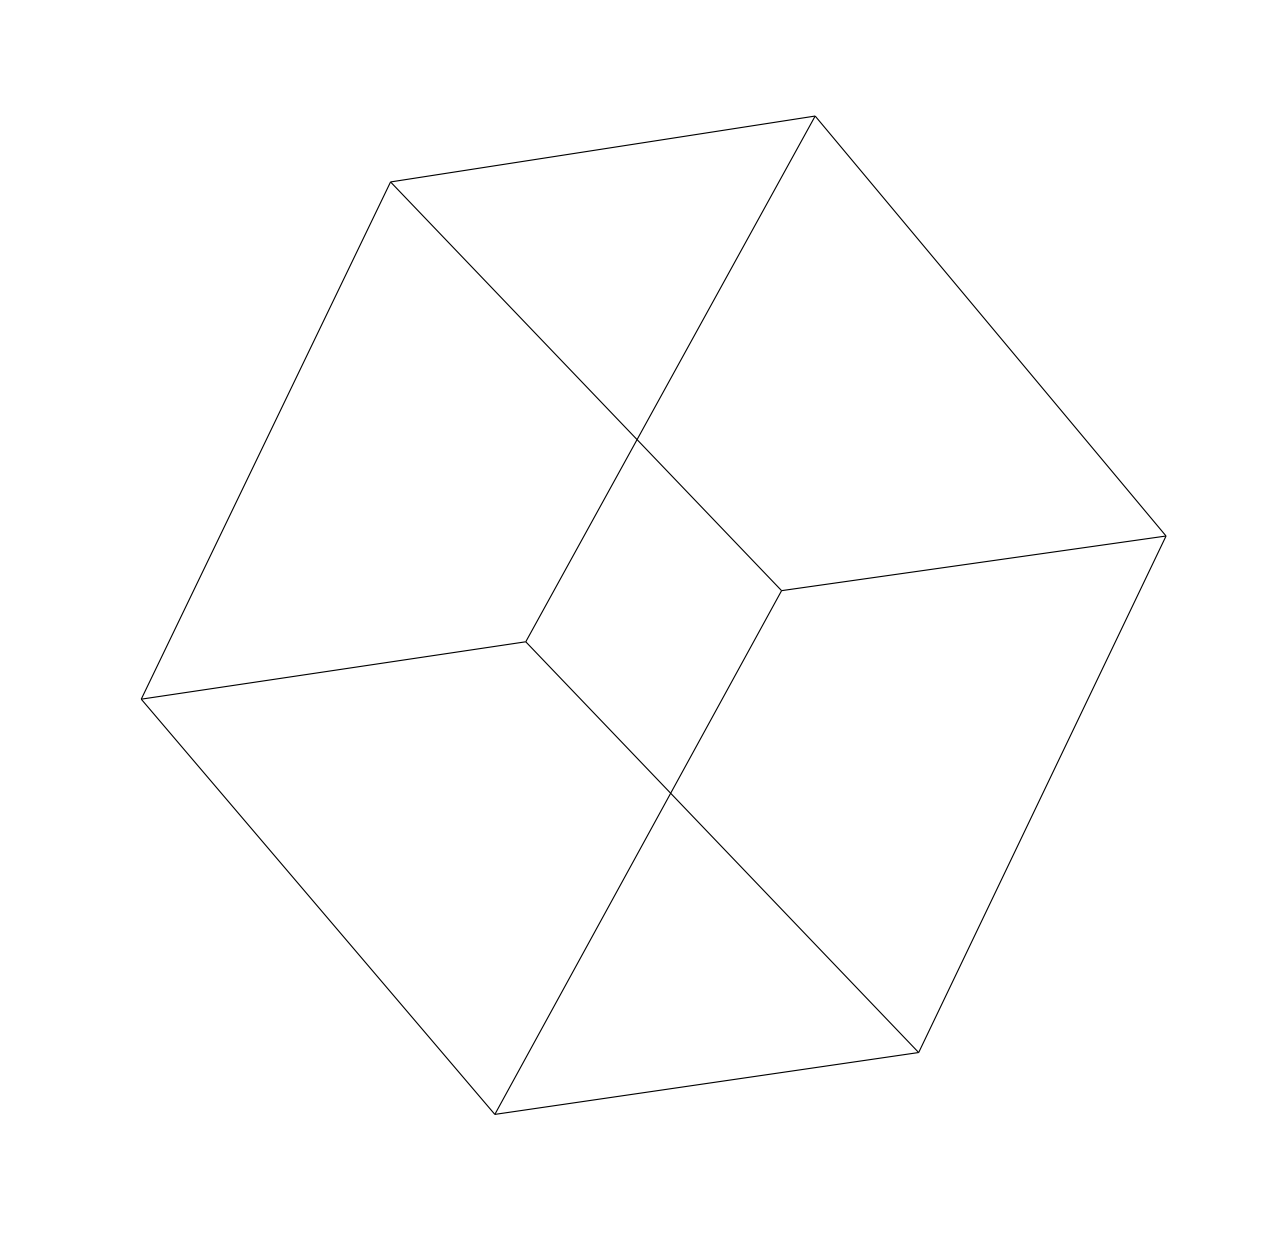
\includegraphics[width=2.2in]{./images02/new-images/qn3.png}}
  \subfloat[$Q_7$]{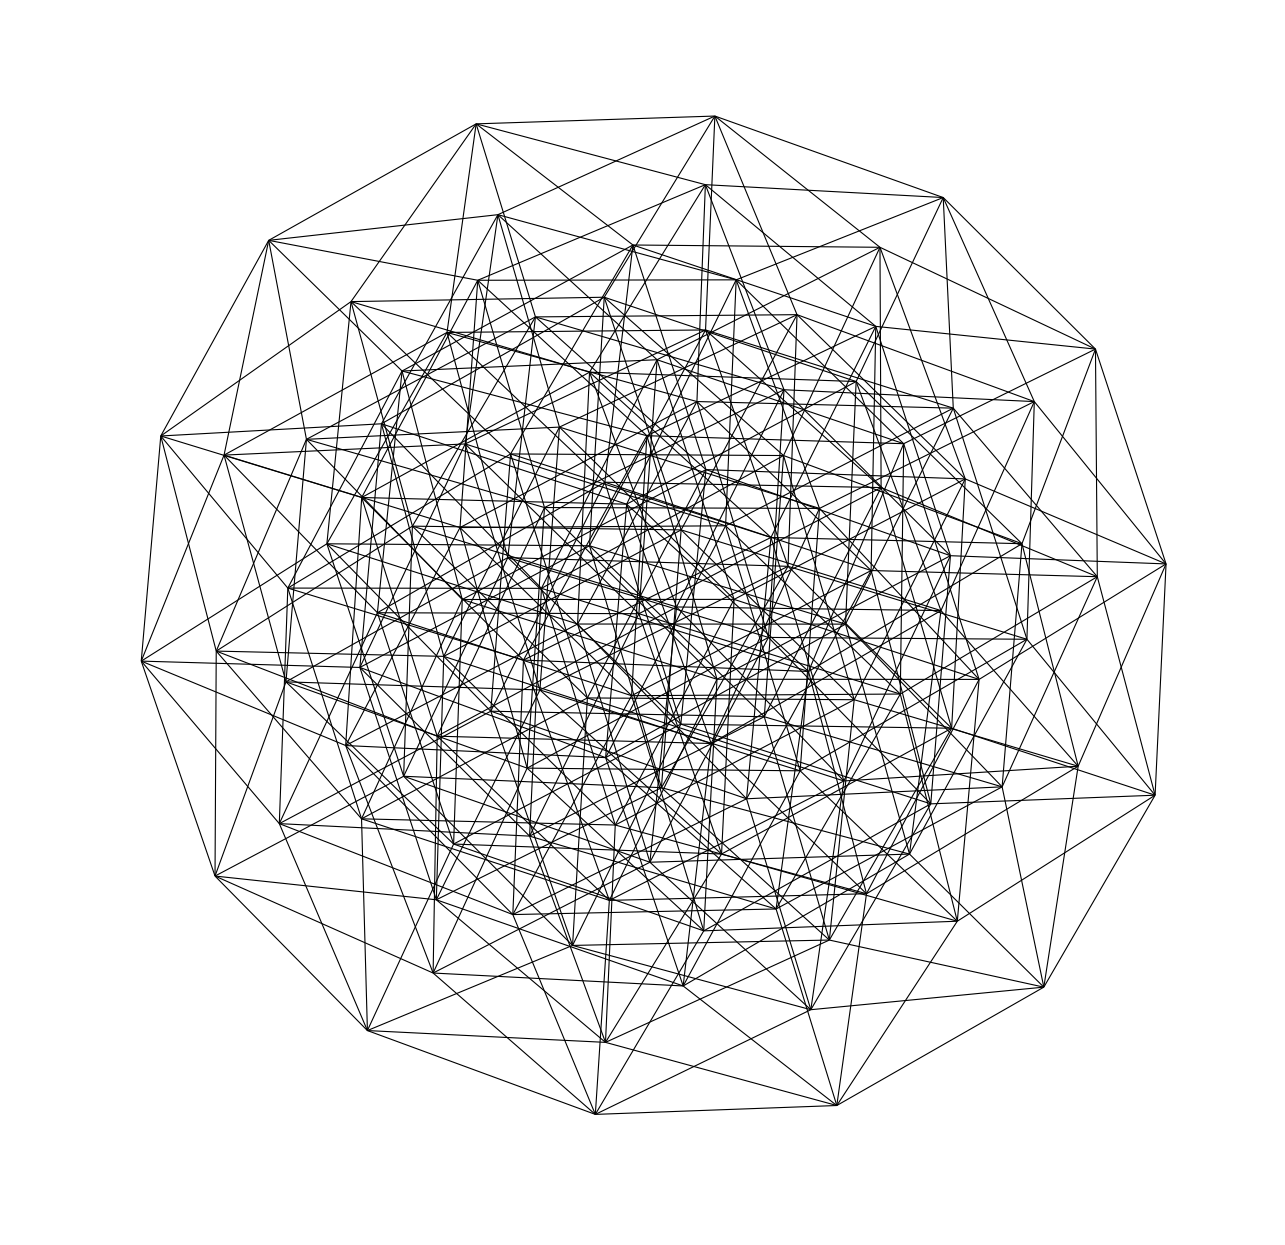
\includegraphics[width=2.2in]{./images02/new-images/qn7.png}}

  \subfloat[$Q_{10}$]{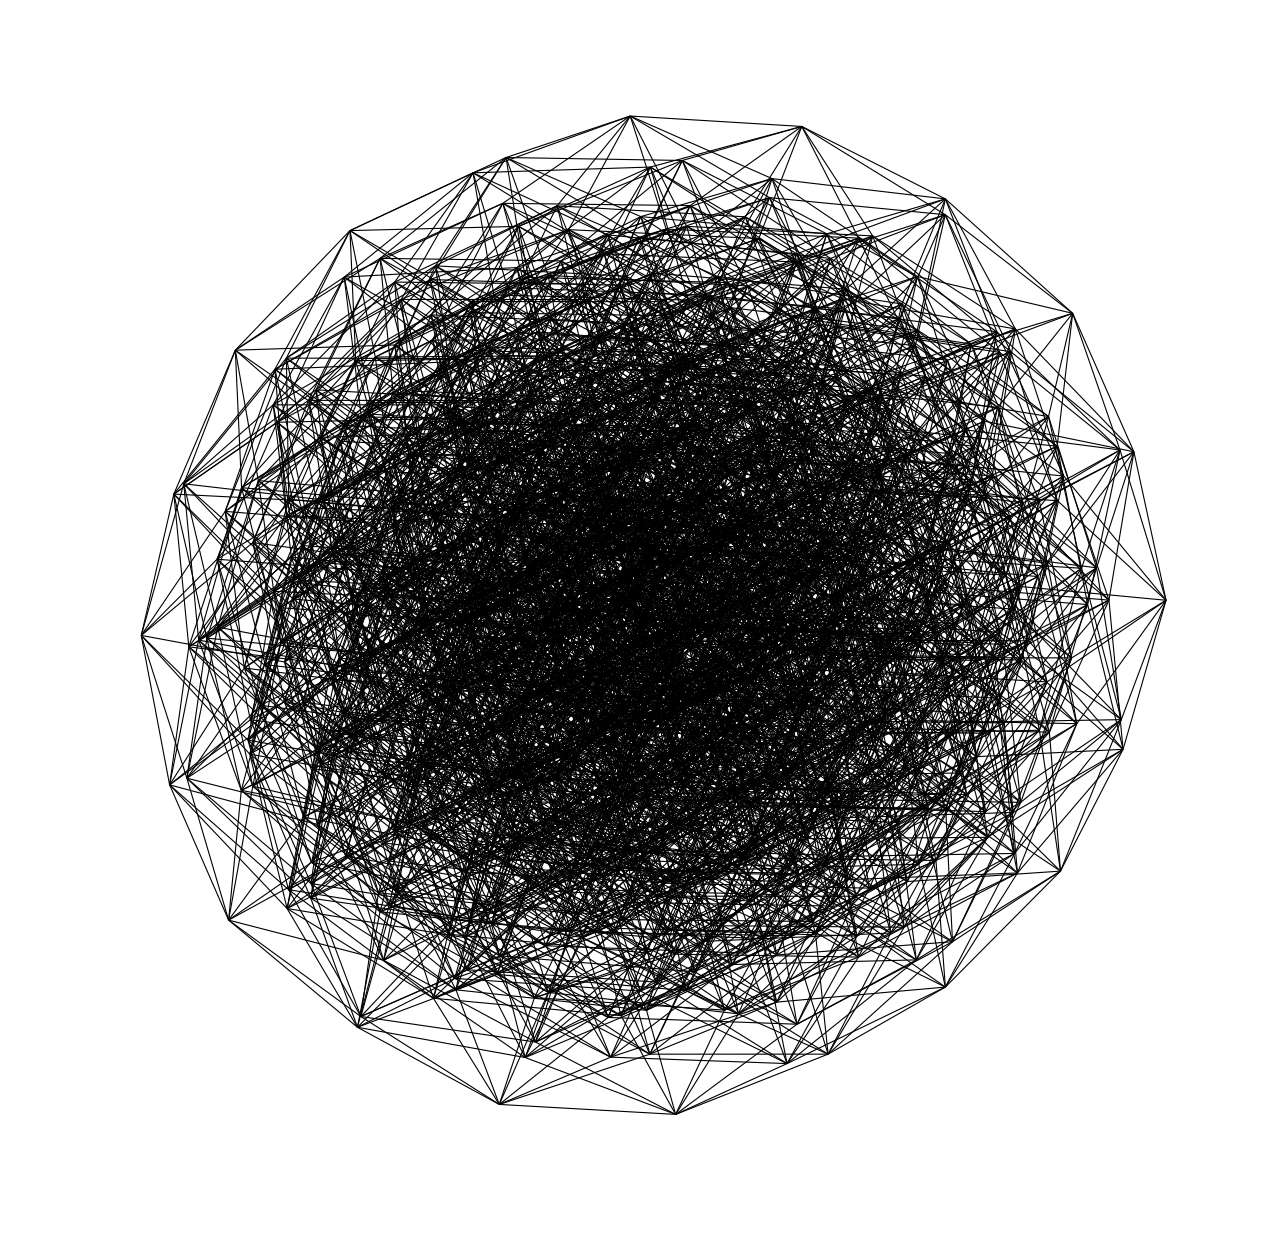
\includegraphics[width=4.0in]{./images02/new-images/qn10.png}}
  \caption{Here we have $Q_n$, for $n \in$ \{3, 7, 10\}. Each node represents a possible bitstring in $\{0,1\}^n$, and two nodes are linked if the bitstrings differ by a single dimension.  A number of observations can be made here. First, the number of nodes grows as $2^n$ as $n$ grows; which makes use of the entire space infeasible as $n>>20$. Another interesting observation, better seen in the figures below, is that most of the space lies at the center, at a distance of around 500 from any given vantage point.\label{hypercubes}}
\end{figure}



The graph composed of $\{0,1\}^n$ nodes and links between nodes $iff$ their Hamming distance is one is called the \emph{hypercube graph}, or $Q_n$, as in Figure \ref{hypercubes}.  Though Kanerva has derived many combinatorial properties of the space, I believe that this is a aesthetically appealing object on its own, and beautiful results can be found in the graph-theoretical literature. A good survey is found in \citet{harary1988survey}.


Here is an interesting question that I leave for further research: A hypercube with n dimensions can be divided by two hypercubes with $n-1$ dimensions. Is there an algorithm that separates the area of each hard-location in such a form that there exists a function mapping each bitstring in $\{0,1\}^n$ to the set of hard locations it belongs to?  In other words… though this would break Kanerva's assumption of a uniformly distributed set of hard locations for a perfectly symmetrical set of hard locations, there could be large performance gains if such a mapping function from a bitstring to its corresponding set of nearest hard locations exists.





Unlike traditional memory used by computers, SDM performs read and write operations in a multitude of addresses, also called neurons.  That is, the data is not written, or it is not read in a single address spot, but in many addresses. These are called activated addresses, or activated neurons.

The activation of addresses takes place according to their distances from the datum. Suppose one is writing datum $\eta$ at address $\xi$, then all addresses inside a circle with center $\xi$ and radius $r$ are activated. So, $\eta$ will be stored in all these activated addresses, which are around address $\xi$, such as in Figure \ref{fig-addresses-inside-access-radius}.  An address $\xi'$ is inside the circle if its hamming distance to the center $\xi$ is less than or equal to the radius $r$, i.e. $distance(\xi,\xi')\leq r$.

\begin{figure}[!htb]
\centering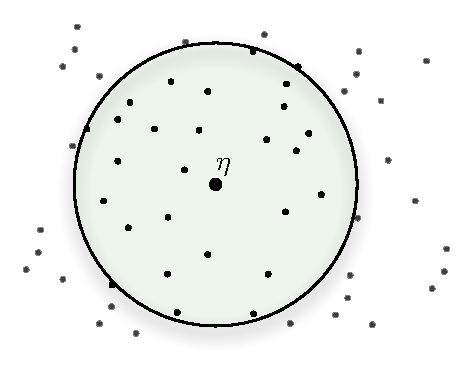
\includegraphics[scale=0.75]{./images02/p_circle_r.pdf}

\caption{Activated addresses inside access \protect \\
radius $r$ around center address.\label{fig-addresses-inside-access-radius}}
\end{figure}



Every time write or read in SDM memory activates a number of addresses with close distance.  The data is written in these activated addresses or read from them.  These issues will be addressed in due detail further on, but a major difference from a traditional computer memory is that the data are always stored and retrieved in a multitude of addresses. This way SDM memory has robustness against loss of addresses (e.g., death of a neuron).

In traditional memory, each datum is stored in an address and every look up of a specific datum requires a search through the memory. In spite of computer scientists having developed beautiful algorithms to perform fast searches, almost all of them do a precise search. That is, if you have an imprecise clue of what you need, these algorithms will simply fail.

In SDM, the data space is the same as the address space, which amounts to a vectorial, binary space, that is, a $\{0,1\}^{n}$ space. This way, the addresses where the data will be written are the same as the data themselves. For example, the datum $\eta=00101_{b}\in\{0,1\}^{5}$ will be written to the address $\xi=\eta=00101_{b}$. If one chooses a radius of 1, the SDM will activate all addresses one bit away or less from the center address. So, the datum $00101_{b}$ will be written to the addresses $00101_{b}$, $10101_{b}$, $01101_{b}$, $00001_{b}$, $00111_{b}$, and $00100_{b}$.

In this case, when one needs to retrieve the data, one could have an imprecise cue at most one bit away from $\eta$, since all addresses one bit away have $\eta$ stored in themselves.  Extending this train of thought for larger dimensions and radius, exponential numbers of addresses are activated and one can see why SDM is a distributed memory.

When reading a cue $\eta_{x}$ that is $x$ bits away of $\eta$, the cue shares many addresses with $\eta$. The number of shared addresses decreases as the cue's distance to $\eta$ increases, in other words, as $x$ increases. This is shown in Figure \ref{fig-shared-addresses}.  The target datum $\eta$ was written in all shared addresses, thus they will bias the read output in the direction of $\eta$. If the cue is sufficiently near the target datum $\eta$, the read output will be closer to $\eta$ than $\eta_{x}$ was. Repeating the read operation increasingly gets results closer to $\eta$, until it is exactly the same. So, it may be necessary to perform more than one read operation in order to converge to the target data $\eta$.

\begin{figure}[!htb]
\centering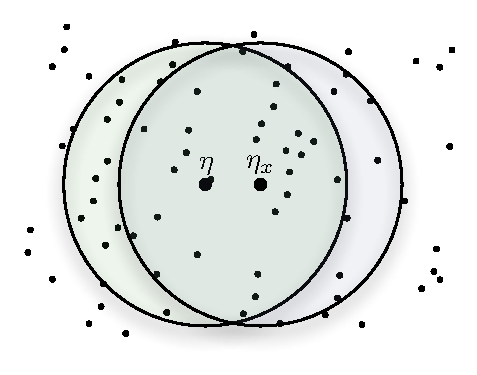
\includegraphics[scale=0.75]{./images02/p1_inter_p2.pdf}

\caption{Shared addresses between the \protect \\
target datum $\eta$ and the cue $\eta_{x}$. \label{fig-shared-addresses}}
\end{figure}


The addresses of the $\{0,1\}^{n}$ space grows exponentially with the number of dimensions $n$, i.e. $N=2^{n}$. For $n=100$ we have $N\approx10^{30}$, which is incredibly large when related to a computer memory. Furthermore, \citet{Kanerva1988} suggests $n$ between 100 and 10,000. Recently he has postulated 10,000 as a desirable minimum $N$ (personal communication). To solve the feasibility problem of implementing this memory, Kanerva made a random sample of $\{0,1\}^{n}$, in his work, having $N'$ elements. All these addresses in the sample are called hard-locations. Other elements of $\{0,1\}^{n}$, not in $N'$, are called virtual neurons. This is represented in Figure \ref{fig-hardlocations}.  All properties of read and write operations presented before remain valid, but limited to hard-locations. Kanerva suggests taking a sample of about one million hard-locations.

Using this sample of binary space, our data space does not exist completely.  That is, the binary space has $2^{n}$ addresses, but the memory is far away from having these addresses available. In fact, only a fraction of this vectorial space is actually instantiated. Following Kanerva's suggestion of one million hard-locations, for $n=100$, only $100\cdot10^{6}/2^{100}=7\cdot10^{-23}$ percent of the whole space exists, and for $n=1,000$ only $100\cdot10^{6}/2^{1000}=7\cdot10^{-294}$ percent.

Kanerva also suggests the selection of a radius that will activate, on average, one one thousandth of the sample, which is 1,000 hard-locations for a sample of one million addresses. In order to achieve his suggestion, a 1,000-dimension memory uses an access radius $r=451$, and a 256-dimensional memory, $r=103$. We think that a 256-dimensional memory may be important because it presents conformity to Miller's magic number \citep{Linhares2011}.

\begin{figure}[!htb]
\centering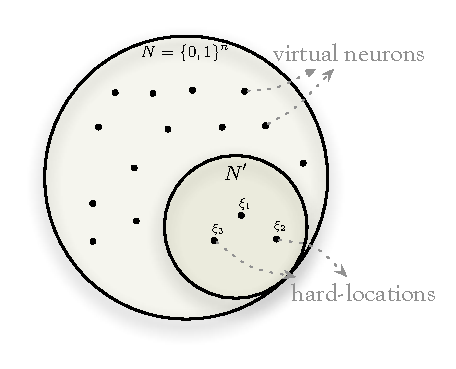
\includegraphics[scale=0.75]{./images02/hardlocations.pdf}

\caption{Hard-locations randomly sampled from binary space.\label{fig-hardlocations}}
\end{figure}


Since a cue $\eta_{x}$ near the target bitstring $\eta$ shares many hard-locations with $\eta$, SDM can retrieve data from imprecise cues. Despite this feature, it is very important to know how imprecise this cue could be while still giving accurate results. What is the maximum distance from our cue to the original data that still retrieves the right answer? An interesting approach is to perform a read operation with a cue $\eta_{x}$, that is $x$ bits away from the target $\eta$.  Then measure the distance from the read output and $\eta$. If this distance is smaller than $x$ we are converging. Convergence is simple to handle, just read again and again, until it converges to the target $\eta$. If this distance is greater than $x$ we are diverging. Finally, if this distance equals $x$ we are in a tip-of-the-tongue process.  A tip-of-the-tongue psychologically happens when you know that you know, but you can't say what exactly it is. In SDM mathematical model, a tip-of-the-tongue process takes infinite time to converge. \citet{Kanerva1988} called this $x$ distance, where the read's output averages $x$, the critical distance. Intuitively, it is the distance from which smaller distances converge and greater distances diverge. In Figure \ref{fig-p1-p2-iterative-read}, the circle has radius equal to the critical distance and every $\eta_{x}$ inside the circle should converge.  The figure also shows a convergence in four readings.

\begin{figure}[!htb]
\centering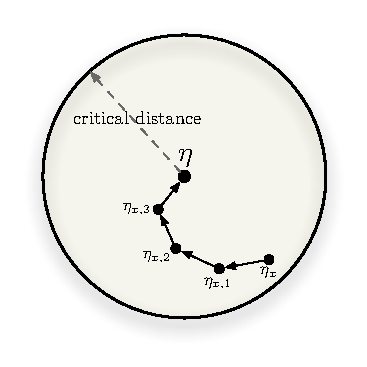
\includegraphics[scale=0.75]{./images02/p1_p2_iter_read.pdf}

\caption{In this example, four iterative readings were\protect \\
required to converge from $\eta_{x}$ to $\eta$.\label{fig-p1-p2-iterative-read}}
\end{figure}


The $\{0,1\}^{n}$ space has $N=2^{n}$ locations from which we instantiate $N'$ samples. Each location in our sample is called a hard-location.  On these hard-locations we do operations of read and write. One of the insights of SDM is exactly the way we read and write: using data as addresses in a distributed fashion. Each datum $\eta$ is written in every activated hard-location inside the access radius centered on the address, that equals datum, $\xi=\eta$. Kanerva suggested using an access radius $r$ having about one one thousandth of $N'$.  As an imprecise cue $\eta_{x}$ shares hard-locations with the target bitstring $\eta,$ it is possible to retrieve $\eta$ correctly. (Actually, probably more than one read is necessary to retrieve exactly $\eta.)$.  Moreover, if some neurons are lost, only a fraction of the datum is lost and it is possible that the memory can still retrieve the right datum.

A random bitstring is generated with equal probability of $0$'s and $1$'s in each bit. One can readily see that the average distance between two random bitstrings has binomial distribution with mean $n/2$ and standard deviation $\sqrt{n/4}$. For a large $n$, most of the space lies close to the mean and has fewer shared hard-locations.  As two bitstrings with distance far from $n/2$ are very improbable, \citet{Kanerva1988} defined that two bitstrings are orthogonal when their distance is $n/2$.

The write operation needs to store, for each dimension bit which happened more ($0$'s or $1$'s). This way, each hard-location has $n$ counters, one for each dimension. The counter is incremented for each bit $1$ and decremented for each bit $0$. Thus, if the counter is positive, there have been more $1$'s than $0$'s, if the counter is negative, there have been more $0$'s than $1$'s, and if the counter is zero, there have been an equal number of $1$'s and $0$'s. Table \ref{tab:write operation} shows an example of a write operation being performed in a 7-dimensional memory.

\begin{table}
\begin{tabular}{c|c|c|c|c|c|c|c|}
\cline{2-8}
$\eta$ & 0 & 1 & 1 & 0 & 1 & 0 & 0\tabularnewline
\cline{2-8}
$\xi_{\textit{before}}$ & 6 & -3 & 12 & -1 & 0 & 2 & 4\tabularnewline
\cline{2-8}
\multicolumn{1}{c}{} & \multicolumn{1}{c}{\textcolor{red}{\small{}$\Downarrow$ -1}} & \multicolumn{1}{c}{\textcolor{red}{\small{}$\Downarrow$ +1}} & \multicolumn{1}{c}{\textcolor{red}{\small{}$\Downarrow$ +1}} & \multicolumn{1}{c}{\textcolor{red}{\small{}$\Downarrow$ -1}} & \multicolumn{1}{c}{\textcolor{red}{\small{}$\Downarrow$ +1}} & \multicolumn{1}{c}{\textcolor{red}{\small{}$\Downarrow$ -1}} & \multicolumn{1}{c}{\textcolor{red}{\small{}$\Downarrow$ -1}}\tabularnewline
\cline{2-8}
$\xi_{\textit{\textit{after}}}$ & \textbf{5} & \textbf{-2} & \textbf{13} & \textbf{-2} & \textbf{1} & \textbf{1} & \textbf{3}\tabularnewline
\cline{2-8}
\end{tabular}

\caption{Write operation example in a 7-dimensional memory of data $\eta$
being written to $\xi$, one of the activated addresses.\label{tab:write operation}}


\end{table}


The read is performed polling each activated hard-location and statistically choosing the most written bit for each dimension. It consists of adding all $n$ counters from the activated hard-locations and, for each bit, choosing bit 1 if the counter is positive, choose bit 0 if the counter if negative, and randomly choose bit 0 or 1 if the counter is zero.


\section{Neurons as pointers}

One interesting view is that neurons in SDM work like pointers. As we write bitstrings in memory, the hard-locations' counters are updated and some bits are flipped. Thus, the activated hard-locations do not necessarily point individually to the bitstring that activated it, but together they point correctly. In other words, the read operation depends on many hard-locations to be successful. This effect is represented in Figure \ref{fig-p1-pointers}: where all hard-locations inside the circle are activated and they, individually, do not point to $\eta$.  But, like vectors, adding them up points to $\eta$. If another datum $\nu$ is written into the memory near $\eta$, the shared hard-locations will have information from both of them and would not point to either.  All hard-locations outside of the circle are also pointing somewhere (possibly other data points). This is not shown, however, in order to keep the picture clean and easily understandable.

\begin{figure}[!htb]
\centering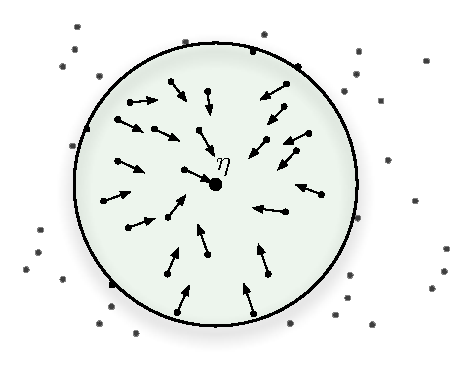
\includegraphics[scale=0.75]{./images02/p1_after_write.pdf}

\caption{Hard-locations pointing, approximately, to the target bitstring.\label{fig-p1-pointers}}
\end{figure}



\section{Concepts}

Although Kanerva does not mention concepts directly in his book \citep{Kanerva1988}, the author's interpretation is that each bitstring may be mapped to a concept. Thus, unrelated concepts are orthogonal and concepts could be linked through a bitstring near both of them. For example, ``beauty'' and ``woman'' have distance $n/2$, but a bitstring that means ``beautiful woman'' could have distance $n/4$ to both of them. As a bitstring with distance $n/4$ is very improbable, it is linking those concepts together. \citet{Linhares2011} approached this concept via ``chunking through averaging''.

Due to the distribution of hard-locations between two random bitstrings, the vast majority of concepts is orthogonal to all others. Consider a non-scientific survey during a cognitive science seminar, where students asked to mention ideas unrelated to the course brought up terms like birthdays, boots, dinosaurs, fever, executive order, x-rays, and so on. Not only are the items unrelated to cognitive science, the topic of the seminar, but they are also unrelated to each other.

For any two memory items, one can readily find a stream of thought relating two such items (``Darwin gave dinosaurs the boot''; ``she ran a fever on her birthday''; ``isn't it time for the Supreme Court to x-ray that executive order?'', ... and so forth). Robert French presents an intriguing example in which one suddenly creates a representation linking the otherwise unrelated concepts of ``coffee cups'' and ``old elephants'' \citep{French1997}.

This mapping from concepts to bitstrings brings us two main questions: (i) Suppose we have a bitstring that is linking two major concepts.  How do we know which concepts are linked together? (ii) From a concept bitstring how can we list all concepts that are somehow linked to it? This second question is called the problem of spreading activation.


\section{Read operation}

In his work, Kanerva proposed and analyzed a read algorithm called here Kanerva's read. His read takes all activated hard-locations counters and sum them. The resulting bitstring has bit $1$ where the result is positive, bit $0$ where the result is negative, and a random bit where the result is zero. In a word, each bit is chosen according to all written bitstrings in all hard-locations, being equal to the bit more appeared. Table \ref{tab:kanerva-read} shows an example of Kanerva's read result bitstring.

Daniel Chada, one member of our research group, proposed another way to read in SDM, in this work called Chada's read. Instead of summing all hard-location counters, each hard-location evaluates its resulting bitstring individually. Then, all resulting bitstrings are summed again, and the same rule as Kanerva applies. Table \ref{tab:chada-read} shows an example of Chada's read result bitstring. The counter's values are normalized to 1, for positive ones, or -1, for negative ones, and the original values are the same as in Table \ref{tab:kanerva-read}.

The main change between Kanerva's read and Chada's read is that, in the former, a hard-location that has more bitstrings written has a greater weight in the decision of each bit. In the latter, all hard-locations have the same weight, because they can contribute to the sum with only one bitstring.

A member of my Master's committee, professor Paulo Murilo, has proposed a generalized reading operation (personal communication), which covers both Kanerva's and Chada's read --- and opens a new venue of potential discoveries. He proposed summing all hard-location counters raised to the power of $z$ while holding the original sign of the counter (positive or negative). Thus, Kanerva's read would be the same as $z=1$, while Chada's would be the same as $z=0$. Hence, we will here explore how SDM would behave with other values of $z$, such as 0.5, 2, and 3.

\begin{table}
\begin{minipage}[t]{0.5\columnwidth}%
\subfloat[Kanerva's read example\label{tab:kanerva-read}]{%
\begin{tabular}{c|c|c|c|c|c|}
\cline{2-6}
$\xi_{1}$ & -2 & 12 & 4 & 0 & -3\tabularnewline
\cline{2-6}
$\xi_{2}$ & -5 & -4 & 2 & 8 & -2\tabularnewline
\cline{2-6}
$\xi_{3}$ & -1 & 0 & -1 & -2 & -1\tabularnewline
\cline{2-6}
$\xi_{4}$ & 3 & 2 & -1 & 3 & 1\tabularnewline
\hline
\multicolumn{1}{|c|}{\textbf{$\sum$}} & \textbf{-5} & \textbf{10} & \textbf{4} & \textbf{3} & \textbf{-5}\tabularnewline
\hline
\multicolumn{1}{c}{} & \multicolumn{1}{c}{\textcolor{red}{\small{}$\Downarrow$}} & \multicolumn{1}{c}{\textcolor{red}{\small{}$\Downarrow$}} & \multicolumn{1}{c}{\textcolor{red}{\small{}$\Downarrow$}} & \multicolumn{1}{c}{\textcolor{red}{\small{}$\Downarrow$}} & \multicolumn{1}{c}{\textcolor{red}{\small{}$\Downarrow$}}\tabularnewline
\cline{2-6}
 & 0 & 1 & 1 & 1 & 0\tabularnewline
\cline{2-6}
\end{tabular}

}%
\end{minipage}%
\begin{minipage}[t]{0.5\columnwidth}%
\subfloat[Chada's read example\label{tab:chada-read}]{%
\begin{tabular}{c|c|c|c|c|c|}
\cline{2-6}
$\xi_{1}$ & -1 & 1 & 1 & \cellcolor{lightgray}1 & -3\tabularnewline
\cline{2-6}
$\xi_{2}$ & -1 & -1 & 1 & 1 & -1\tabularnewline
\cline{2-6}
$\xi_{3}$ & -1 & \cellcolor{lightgray}1 & -1 & -1 & -1\tabularnewline
\cline{2-6}
$\xi_{4}$ & 1 & 1 & -1 & -1 & 1\tabularnewline
\hline
\multicolumn{1}{|c|}{\textbf{$\sum$}} & \textbf{-2} & \textbf{1} & \textbf{0} & \textbf{0} & \textbf{-2}\tabularnewline
\hline
\multicolumn{1}{c}{} & \multicolumn{1}{c}{\textcolor{red}{\small{}$\Downarrow$}} & \multicolumn{1}{c}{\textcolor{red}{\small{}$\Downarrow$}} & \multicolumn{1}{c}{\textcolor{red}{\small{}$\Downarrow$}} & \multicolumn{1}{c}{\textcolor{red}{\small{}$\Downarrow$}} & \multicolumn{1}{c}{\textcolor{red}{\small{}$\Downarrow$}}\tabularnewline
\cline{2-6}
 & 0 & 1 & \cellcolor{lightgray}1 & \cellcolor{lightgray}1 & 0\tabularnewline
\cline{2-6}
\end{tabular}

}%
\end{minipage}\caption{Comparison of Kanerva's read and Chada's read. Each $\xi_{i}$ is
an activated hard-location and the values come from their counters.
Gray cells' value is obtained randomly with probability 50\%.\label{tab:read-operation}}
\end{table}


\section{Critical Distance}

Kanerva describes the critical distance as the threshold of convergence of a sequence of read words. It is ``the distance beyond which divergence is more likely than convergence''\citep{Kanerva1988}. Furthermore, Kanerva explains that ``a very good estimate of the critical distance can be obtained by finding the distance at which the arithmetic mean of the new distance to the target equals the old distance to the target''\citep{Kanerva1988}.  In other words, the critical distance can be equated as the edge to our memory, the limit of human recollection.

In his book, Kanerva analyzed a specific situation with $n=1000$ ($N=2^{1000}$), 10 million hard-locations, an access-radius of 451 (within 1000 hard-locations in each circle) and 10 thousand writes of random bitstrings in the memory. As computer resources were very poor those days, Kanerva couldn't make a more generic analysis.

Starting from the premise of SDM as a faithful model of human short-term memory, a better understanding of the critical distance may shed light on our understanding of the thresholds that bind our own memory.


\begin{figure}[!htb]
\centering

\subfloat[Kanerva's original model]{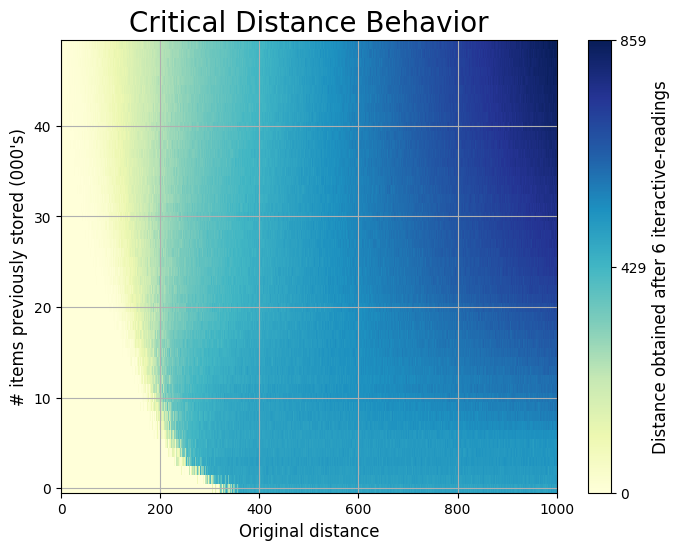
\includegraphics[width=3.1in]{./images02/new-images/kanerva-read.png}}

\subfloat[Chada's read]{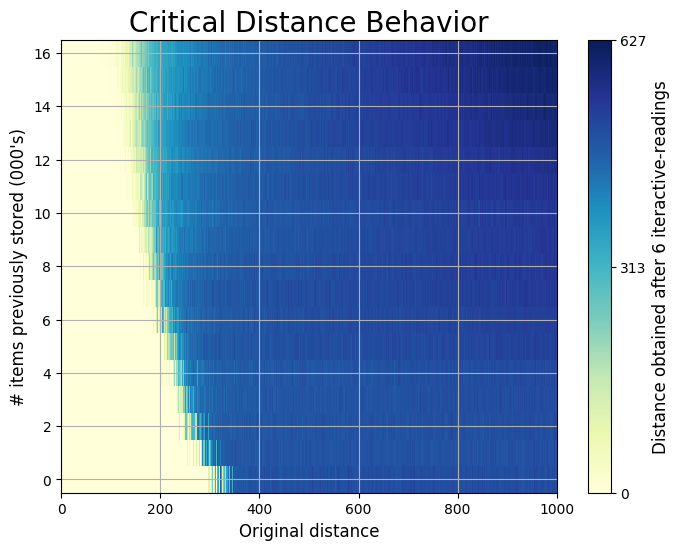
\includegraphics[width=3.1in]{./images02/new-images/chada-read_z_0.png}}
\caption{How far, in hamming distance, is a read item from the original stored item? Kanerva demonstrated that, after a small number of iterative readings (6 here), a critical distance behavior emerges. Items read at close distance converge rapidly; whereas farther items do not converge. Most striking is the point in which the system displays the tip-of-tongue behavior. Described by psychological moments when some features of the item are prominent in one's thoughts, yet the item still cannot be recalled (but an additional cue makes convergence `immediate'). Mathematically, this is the precise distance in which, despite having a relatively high number of cues (correct bits) about the desired item, the time to convergence is infinite.   Heatmap colors display the hamming distance the associative memory is able to cleanly converge to---or not.   In the $x$-axis, the distance from the desired item is displayed. In the $y$-axis, we display the read operation's behavior as the number of items registered in the memory grows.  These graphs are computing intensive, yet they can be easily tested by readers in our provided jupyter notebooks. Note the different scales.}
\label{fig:crit-dist-10k-writes}

\end{figure}

Figure \ref{fig:crit-dist-10k-writes} compares the critical distance behavior under different scenarios.  This replicates our previous results \citet{Brogliato2011} and \citet{brogliato2014sparse} and is a first part of the process of framework validation, to which we throw our attention next.



\chapter{Framework Architecture}

The framework implements the basic operations in a Sparse Distributed Memory which may be used to create more complex operations. It is developed in C language and the OpenCL parallel framework --- which may be loaded in many platforms and programming languages --- with a wrapper in Python. The Python module makes it easy to create and execute simulations in a Sparse Distributed Memory and works properly in Jupyter Notebook \citep{kluyver2016jupyter}. It works in both Python 2 and Python 3.

We split the SDM memory in two parts: the hard-location addresses and the hard-location counters. Thus, the addresses (bitstrings) of the hard-locations are stored in one array, while their counters in another. This makes possible to create multiple SDMs using the same address space, which would save computational effort to scan a bitstring in all the SDMs --- since they share the same address space, the activated hard-locations will be the same in all of them. As the slowest part of reading and writing operations is scanning the address space, the performance benefits are significant.

Each part may be stored either in the RAM memory or in a file. The RAM memory is interesting for quick experiments, automated tests, and others scenarios in which the SDM may be lost, while the file is interesting for a long-term SDM, like creating an SDM file with 10,000 random writes, which will be copied over and over to run multiple experiments. The file may also be sent to another researcher or may be published within the paper to let others run their own checks and verify the results. In summary, the framework fits many different uses and necessities.

Let a SDM memory with $N$ dimensions and $H$ hard-locations. Then, in a 64-bit computer, the array of hard-location addresses will use $H \cdot 8 \cdot \lceil N/64 \rceil$ bytes of memory, and there will be $H \cdot N$ hard-location counters. For example, in a SDM memory with 1,000 dimensions and 1,000,000 hard-locations, using 32-bit integers for the counters, the array of addresses will use 122MB of memory and the counters will use 3.8 GB of memory.

Basic operations were grouped in four sets: (i) for bitstrings, (ii) for addresses, (iii) for counters, and (iv) for memories (SDMs). Operations include creating new bitstrings, flipping bits, generating a bitstring with a specific distance from a given bitstring, scanning the address space using different algorithms, writing a bitstring to a counter, writing in an SDM, reading from an SDM, and iteratively reading from an SDM until convergence.


\section{Bitstring}

Bitstrings are the main structure of SDM. The addresses are represented in bitstrings, as well as the data. A bitstring is stored as an array of integers. Each integer may be 16-bit, 32-bit, or 64-bit long, depending on the configuration. By default, each integer is 64-bit long.

For instance, a 1,000-bit bitstring will have $\lceil 1000/64 \rceil = 16$ integers. These integers will have a total of $16 \cdot 64 = 1,024$ bits. The remaining 24 bits are always zero, so they do not affect the result of any operation. The memory usage efficiency is $1 - 24/1024 = 97.65\%$. Bitstrings store neither how many bits they have nor the array length. These pieces of information are only stored in the address space.


\subsection{The distance between two bitstrings}

The distance between two bitstrings is calculated by the hamming distance, which is the number of different bits between them. It is calculated counting the number of ones in the exclusive or (xor) between the bitstrings, i.e., $d(x, y) = \text{number of ones in } x \oplus y$.

There are several algorithms to calculate the number of ones \citep{warren2013hacker}, but the performance depends on the processor. So, we have implemented three different algorithms and one may be selected through compiling flags. The default algorithm is to use a built-in \_\_popcnt() instruction from the compiler.

There is also the naive algorithm, which really counts the number of ones checking bit by bit. It is available only to testing purposes and should never be used.

The other algorithm available is the lookup. It pre-calculates a table with the number of ones of all possible 16-bit integers. This table is accessed a few times to calculate the number of ones of a 64-bit integer, i.e., to calculate the distance between two bitstrings, it sums the distance of each 16-bit part of the bitstrings, i.e., $d(x[0:63], y[0:63]) = d(x[0:15], y[0:15]) + d(x[16:31], y[16:31]) + d(x[32:47], y[32:47]) + d(x[48:63], y[48:63])$ where $x[i:i+15]$ and $y[i, i+15]$ are the 16-bit integers formed by the bits between $i$ and $i+15$ of $x$ and $y$, respectivelly. Each 16-bit distance is calculated through a single table access. As each distance is calculated in O(1), this algorithm runs in O($\lceil bits/16 \rceil$). This table uses 65MB of RAM. One may change the table from 16-bit integers to 32-bit integers, which would halve the number of accesses at the expense of 4GB of RAM (instead of 65MB).


\section{Address space}

An address space is a fixed collection of bitstrings, and each bitstring represents a hard-location address. They store the number of bitstrings, as well as the number of bits, number of integers per bitstring, and the number of remaining bits.

Bitstrings are stored in a contiguous array of 64-bit integers, as shown in Figure \ref{tab:hl-addresses-detail}. Hence, basic pointer arithmetic provides us with performance improvements in their access, as processors realize fetches of contiguous chunks of memory  \citep{pai2004linux}.

\begin{figure}
\centering
\begin{tikzpicture}[
mycell/.style={draw, minimum size=7mm},
matrixA/.style={matrix of nodes,
    nodes={mycell, anchor=center},
    column sep=-\pgflinewidth,
    row sep=-\pgflinewidth,
    },
matrixB/.style={matrix of nodes,
    nodes={mycell, anchor=center},
    column sep=-\pgflinewidth,
    row sep=-\pgflinewidth,
}]

\matrix[matrixA] (A) { addr$_1$ & addr$_2$ & addr$_3$ & $\cdots$ & addr$_H$ \\ };

\matrix[matrixB, below=of A] (B) {
addr$_{k, 1}$ & addr$_{k, 2}$ & addr$_{k, 3}$ & $\cdots$ & addr$_{k, 8 \cdot \lceil N/64 \rceil}$ \\
};

\draw[dashed] (A-1-1.south west)--(B-1-1.north west);
\draw[dashed] (A-1-1.south east)--(B-1-5.north east);
\draw [
	thick,
    decoration={
        brace,
        mirror,
		amplitude=0.2cm,
        raise=0.2cm
    },
    decorate
] (B-1-1.south west) -- (B-1-5.south east)
node [pos=0.5,anchor=north,yshift=-0.5cm] {N bits};

\end{tikzpicture}

\caption{Address space's bitstrings are stored in a contiguous array. In a 64-bit computer, each bitstring is stored in a sub-array of 64-bit integers, with length $8 \cdot \lceil N/64 \rceil$.\label{tab:hl-addresses-detail}}
\end{figure}

The scan for activated hard-locations is performed in an address space. It returns the indexes of the bitstrings which were inside the circle (and their distances). Then, each operation uses these pieces of information in a different way.

\subsection{Scanning for activated hard-locations}

Scanning for the activated hard-locations is a problem similar to well-known problems in computational geometry called ``range reporting in higher dimensions''. In this case, none of the known algorithms is able to solve our problem faster than $O(H)$. The algorithm which seems to best fit in our problem consumes $O(H)$ space and runs in $O(\log^n(H))$ \citep{chazelle1988functional}, which is really slower than $O(H)$ when, for instance, $H=1,000,000$ and $n=1,000$. For a review of the range reporting algorithms, see \citet{chan2011orthogonal}.

In 2014, there was published a solution to fast search in hamming space which seems applicable to our problem \citet{norouzi2014fast}. It provides a fast search when $r/n < 0.11$ or $r/n < 0.06$, where $r$ is the radius and $n$ is the number of bits. But, in our case, for a 1,000 bits SDM, $r/n = 0.451$, which changes the runtime to $O(H^{0.993})$. This is really close to $O(H)$, but with a larger constant. Unfortunately, $O(H)$ is still faster.

It is intriguing that none of those algorithms is able to solve our scanning problem. The idea behind those computational geometry algorithms is roughly to split the search space in half each step, which would take $O(\log(H))$ to go through the whole space. But this approach does not work because of the high number of dimensions (i.e., 1,000) and because the hard-locations' addresses are randomly sampled from the $\{0, 1\}^n$ space. Although each addresses' bit itself splits the hardlocations in half, it does not split the search space in half since both halves still must be convered by the algorithm. For instance, let's say we have $n=1,000$ dimensions with $H=1,000,000$ hard-locations, and we are scanning within a circle with radius $r=451$, then after checking the first bit we have two cases: (i) for the half with the same first bit, we must keep scanning with radius 451; and (ii) for the half with a different first bit, we must keep scanning with radius 450. Hence, the search space has not been split in half because both halves have been covered (and one of them should have been skipped).

Finally, as our best approach is to scan through all hard-locations, we may distribute the scan into many tasks which will be executed independently. The tasks may be executed in different processes, threads, or even computers. They may also run in the CPU or in the GPU. In this case, we may take into account both the time required to distribute the tasks and the time to receive their results.

The framework implements three main scanner algorithms: linear scanner, thread scanner, and OpenCL scanner. The linear scanner runs in a single core, is the slowest one, and was developed only for testing purposes; the thread scanner runs at the CPU in multiple threads sharing memory (and our recommendation is to use the number of threads equals to twice the number of CPU cores); and the OpenCL scanner runs in multiple GPU cores and support multiple devices. The speed of a scan depends on the CPU and GPU devices, thus the best approach to choose which scanner is best for one's setup is to run a benchmark.

The OpenCL must be initialized, which just copies the address space's bitstrings to the GPU's memory. Then, many scans may be executed with no necessity to upload the bitstrings again. The OpenCL scanner supports running into multiple devices.


\section{Counters}

Each hard-location has one integer of data per bit. For instance, each hard-location of a 1,000 bits SDM has 1,000 bits. Those integers are stored in a counter.

A counter is an array of integers which stores the data of all hard-locations. So, the counter's array has $n \cdot H$ integers.

When two counters are added in a third counter, there may occur an overflow. It is not supposed to be a problem because, by default, each counter is a signed 32-bit integer that can store any number between -2,147,483,648 and 2,147,483,647, which means they will not overflow with less writes than $2^{31}-1$ divided by the average number of activated hard-locations. For instance, when $n=1,000$, $H=1,000,000$, and $r=451$, the average number of activated hard-locations is 1,000 and it would require at least one million writes before being possible to a counter to overflow.  Note also that it would be more likely to saturate the memory before any overflow.

Anyway, counters may have overflow protection depending on compiling options. By default, there is no overflow check for performance reasons (and because it does not seem necessary).

\section{Read and write operations}

The reading and writing operations are executed in two steps: first, the address space is swept looking for the activated addresses; then, the operation is performed in the counters. Reading operation assemblies the bitstring according to the counters of the activated addresses, while the writing operation changes the counters.

The iterated reading keeps reading until it gets exactly the same bitstring (or the number of maximum interations has been reached), i.e., it performs $\eta_{i+1} = \text{read}(\eta_i)$ and stops when $\eta_{k+1} = \eta_{k}$. If the initial bitstring is inside the critical distance of $\eta$, it will converge to $\eta$, but, if it is not, it will diverge and reach the maximum number of iterations.

The framework has both Kanerva's read and the generalized read. The latter was implemented according to the generalization proposed by professor Paulo Murilo. The generalization brings a parameter $z$, which is the exponent. In this case, the results are floating point instead of integer, which considerably reduces performance. When $z=1$, it is exactly as the Kanerva's read. When $z=0$, it is the Chada's read. We also explored how SDM would behave for different values of $z$.

There is another special read operation: the weighted reading. In the weighted reading, the value of the counters are multiplied by a weight which depends only on the distance between the reading address and the hard-location address. The weight is retrieved from a lookup table of integers indexed by the distance. The rest of the read operation is exactly the same.

There is also a weighted writing operation. In this case, the weight is applied when the counters are updated, i.e., if the weight is 2, the counters are increased twice when bits are 1, and decreased twice when bits are 0. Just as in the weighted reading, the weights depend only on the distance between the writing address and the hard-location address. The weights are retrieved from a lookup table of integers indexed by the distance.


\chapter{Results (i): Framework Validation}

The framework has been validated comparing its results with the expected results from \citet{Kanerva1988}. Thus, we run simulations which were then compared to the theoretical analysis conducted some decades ago.

\section{Distance between random bitstrings}

As showed by \citet{Kanerva1988}, the distance between two bitstrings follows a binomial distribution with mean $\mu = n/2$ and standard deviation $\sigma = \sqrt{n}/2$. For large values of $n$, it may be approximated by a normal distribution with the same mean and standard deviation.

In order to validate our random bitstring generation algorithm, we have calculated 10,000 distances between two random bitstrings with $n=1,000$ bits. In total, 20,000 random bitstrings have been generated during the simulation. The code is available in the ``Distance between bitstrings'' notebook \citep{sdmframework}.

In figure \ref{fig:validation-distance}, we can notice that the theoretical model and the simulation matches. Hence, it seems the random bitstring generation algorithm works properly.

This also validates the algorithm used to calculate the distance between two bitstrings. In this simulation, we have used the built-in \_\_popcnt() function.

\begin{figure}[!htb]
  \centering
  \subfloat[Full histogram ]{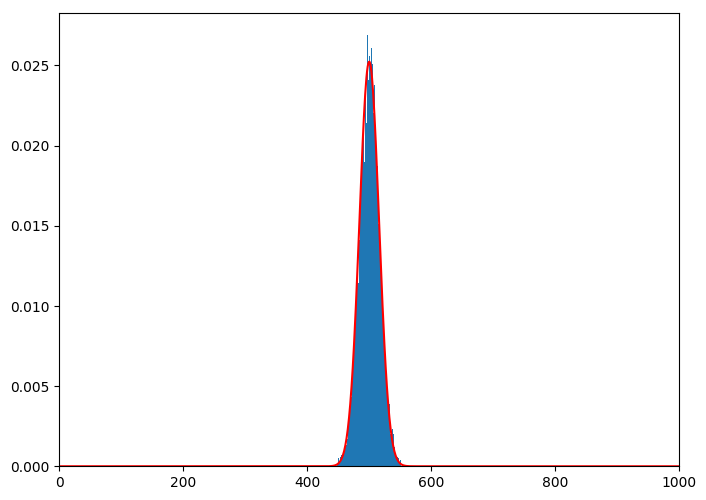
\includegraphics[width=0.5\textwidth]{./images02/new-images/bs-hist-full.png}}
  \subfloat[{Zoom in the interval $[400, 600]$} ]{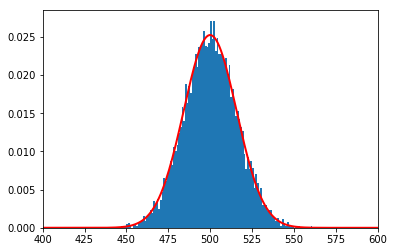
\includegraphics[width=0.5\textwidth]{./images02/new-images/bs-hist-zoom.png}}

  \caption{Histogram of 10,000 distances between two random bitstrings with 1,000 bits. The curve in red is the theoretical normal distribution with $\mu = 500$ and $\sigma = \sqrt{500}/2$.}
  \label{fig:validation-distance}
\end{figure}


\section{Number of activated hard-locations}

In his seminal work, Kanerva proposed to use a sample of 1,000,000 hard-locations in a 1,000 bits SDM. He also proposed to activate only 1,000 of them, on average. He calculated that an access radius of $r=451$ would activate, on average, 0.00107185004892 of the whole space, or, in this case, 1,071.85 hard-locations.

We extended his results, calculating the distribution of the number of activated hard-locations. As each hard-location has probability $p=0.00107185004892$ of being activated, the probability of activating exactly $a$ out of $H$ hard-locations follows a binomial distribution with mean $\mu = pH$ and standard deviation $\sigma = \sqrt{Hp(p-1)}$. In this case, $\mu = 1071.85$ and $\sigma = 32.72$.

In order to validate our scan algorithm, we have run 10,000 scans from a random bitstring and counted the number of activated hard-locations. The code is available in the ``Number of activated hard-locations'' notebook \citep{sdmframework}.

In figure \ref{fig:validation-activated-hls}, we can notice that the theoretical model and the simulation matches. Hence, it seems that both the address space generation algotihm and the scan algorithm work properly. Notice that the curve is almost the same for $n=1,000$ and $n=256$. It happens because the access radius is adjust to have $p$ as close as possible to $0.001$. They are not exactly the same because their $p$ differs a little.

\begin{figure}[!htb]
  \centering
  \subfloat[$n=1,000$, $H=1,000,000$,\protect\\ $r=451$, and $p=0.00107185$ ]{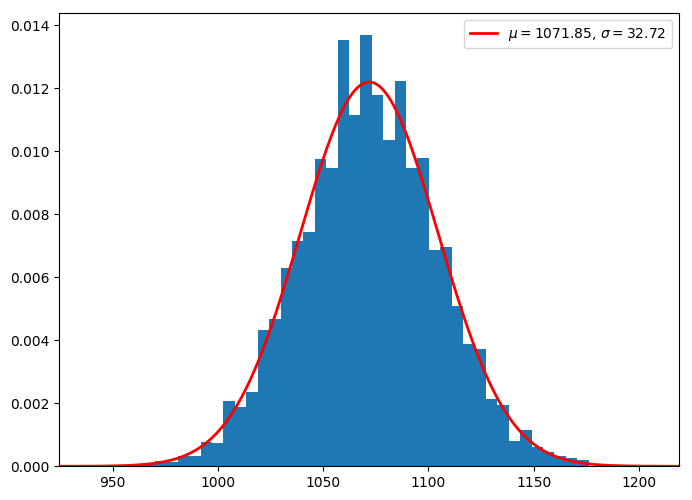
\includegraphics[width=0.5\textwidth]{./images02/new-images/activated-hls-1000.png}}
  \subfloat[$n=256$, $H=1,000,000$,\protect\\ $r=103$, and $p=0.00106684$ ]{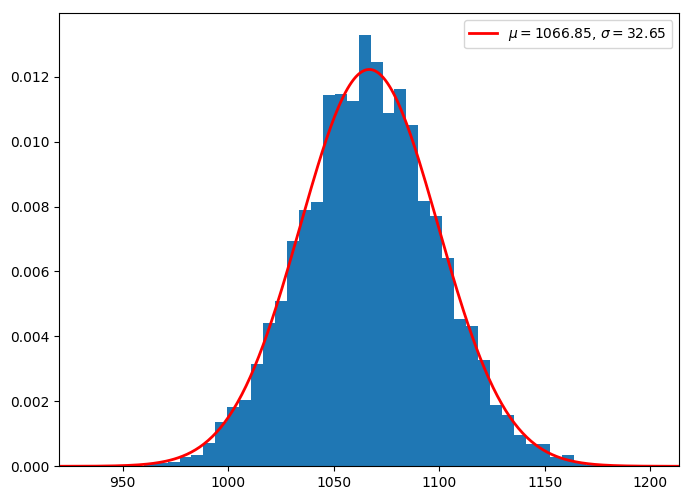
\includegraphics[width=0.5\textwidth]{./images02/new-images/activated-hls-256.png}}

  \caption{Histogram of the number of activated hard-locations in 10,000 scans from a random bitstring. The curve in red is the theoretical normal distribution with $\mu = Hp$ and $\sigma = p(p-1)H$.}
  \label{fig:validation-activated-hls}
\end{figure}

Besides the number of activated hard-locations, we have also extended Kanerva's results to calculate the distribution of distances between the center of the circle and the activated hard-locations. Let $A$ be the set of activated hard-locations, $\xi$ be the center of the circle, and $r$ be the access radius, then:

\begin{align}
P(\text{d}(a, \xi)=x | a \in A) &= \frac{P(\text{d}(a, \xi)=x)}{P(a \in A)} \\
    &= \frac{\binom{n}{x}}{\sum_{k=0}^r \binom{n}{k}} \label{eq:prob-d-inside-circle}
\end{align}

In order to check Equation \ref{eq:prob-d-inside-circle}, we have calculated the distances of the activated hard-locations to the center of 1,000 random circles. The code is available in the ``Distances of activated hard-locations'' notebook \citep{sdmframework}.

In figure \ref{fig:validation-distance-activated-hls}, we can notice that the theoretical model and the simulation matches.

\begin{figure}[!htb]
\centering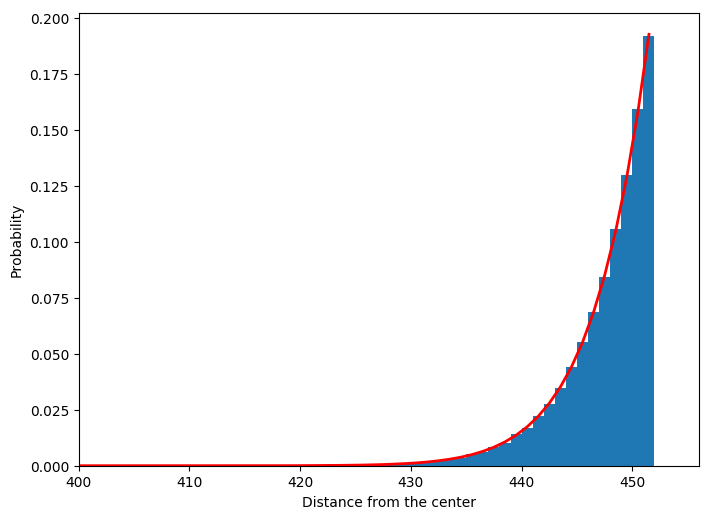
\includegraphics[width=\textwidth]{./images02/new-images/distance-activated-hls.png}

\caption{Histogram of the distances of activated hard-locations to the center of the circles. The curve in red is the theoretical distribution of Equation \ref{eq:prob-d-inside-circle}
\label{fig:validation-distance-activated-hls}}
\end{figure}

\section{Intersection of two circles}

Kanerva has calculated the intersection of two circles according to the distance between their centers. The intersection is important to understand how SDM works, because it affects directly the critical distance. When $\eta_d$ is inside the critical distance, then it will converge to $\eta$. In fact, it converges because they share a sufficient amount of hard-locations, i.e., the intersection of the circle around $\eta_d$ and $\eta$ is enough to converge. For further information about the relation between the critical distance and the intersection, see \citet{brogliato2014sparse}.

We have calculated the intersection between a random bitstring (bs1) and another bitstrings (bs2) exactly $d$ bits away. The former (bs1) is just a random bitstring. The latter (bs2) was generated randomly flipping $d$ bits of bs1. The code is available in the ``Kanerva's Figure 1.2'' notebook \citep{sdmframework}.

In Figure \ref{fig:validation-intersection}, we can notice that we have obtained the same results as Kanerva. It seems that the random flipping bits algorithm and the scan algorithm work properly.

\begin{figure}[!htb]
  \centering
  \subfloat[{\citet[Figure 1.2, p.25]{Kanerva1988}} ]{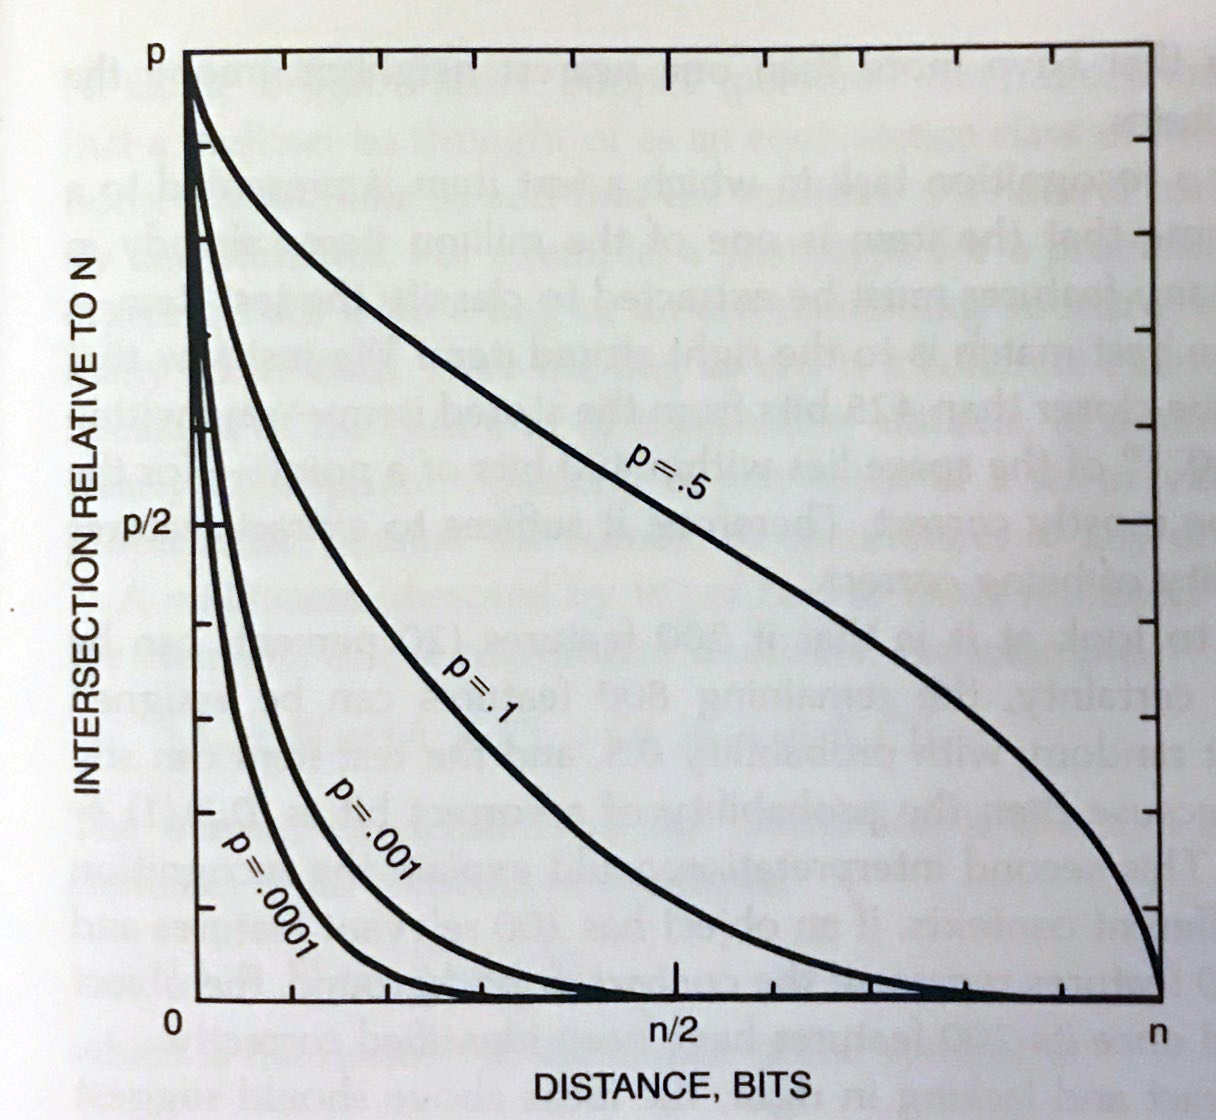
\includegraphics[width=0.45\textwidth]{./images02/new-images/kanerva-table-12.jpg}}
  \subfloat[Generated by SDM-Frameworkm with $n=1,000$ ]{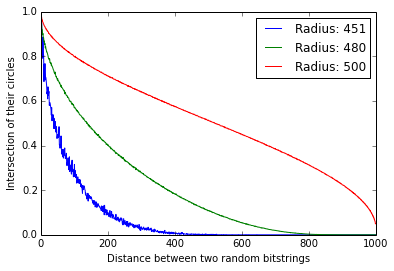
\includegraphics[width=0.55\textwidth]{./images02/new-images/intersection-of-circles.png}}

  \caption{Number of hard-locations in the intersection of circles around two bitstrings $x$ bits away.}
  \label{fig:validation-intersection}
\end{figure}


\section{Storage and retrieval of sequences}

\citet[Ch.8]{Kanerva1988} presented an approach to store and retrieve sequences using $k$ different SDMs, namely $\text{sdm}_1$, $\text{sdm}_2$, $dots$, $\text{sdm}_k$.

Let $a_0, a_1, a_2, \dots, a_n$ be a sequence to be stored in a $k$-fold memory. So, all pointers of the form $a_i \rightarrow a_{i+k}$ will be written to $\text{sdm}_k$ memory, i.e., in $\text{sdm}_1$, the following pointers will be written: $a_0 \rightarrow a_1$, $a_1 \rightarrow a_2$, $\dots$, $a_{n-1} \rightarrow a_n$; while in $\text{sdm}_2$, the following pointers will be written: $a_0 \rightarrow a_2$, $a_2 \rightarrow a_3$, $\dots$, $a_{n-2} \rightarrow a_n$; and so forth.

We have tested exactly the same example presented in \citet{Kanerva1988}, p.85. We wrote two sequences to a $3$-fold memory: $<A, B, C, D>$ and $<E, B, C, F>$. Then, after reading the sequences $<A, B, C>$ and $<E, B, C>$, we have obtained $D$ and $F$, respectively.

Each reading operation was performed summing the counters of all activated hard-locations from all three memories. For instance, to read the sequence $<A, B, C>$, we have activated the hard-locations around $C$ in $\text{sdm}_1$, we have also activated the hard-locations around $D$ in $\text{sdm}_2$, and, finally, we have also activated the hard-locations around $A$ in $\text{sdm}_3$. After summing the counters of all those hard-locations, we evaluate the resulting bitstring just as in the original read operation.

The code is available in the ``Sequences (Kanerva Ch 8)'' notebook \citep{sdmframework}.

The logic behind how it works is that, when reading the sequence $<A, B, C>$, we have $A$ pointing to $D$, while both $B$ and $C$ point to $D$ and $F$. Thus, $D$ appears more often than $F$ and ended up being the result.

Hence, as we have replicated the theoretical results from Kanerva, we have one more evidence that our framework works properly.

\subsection{$k$-fold memory using only one SDM}

We have extended Kanerva's ideas to be able to store and retrieve sequences in $k$-fold memories using only one SDM (instead of $k$ SDMs).

Our idea was to create $k$ random bitstrings, one for each fold. We have performed writing and reading exactly as Kanerva's original idea, but, instead of writing to $\text{sdm}_k$, we have written $a_{i+k}$ into the address $a_i \oplus \text{tag}_k$, and, instead of reading from $\text{sdm}_k$, we have read from address $a_i \oplus \text{tag}_k$, where $\oplus$ is the exclusive or (XOR) operator.

It worked as if we had splitted SDM into $k$ regions with low intersection between two of them. So, as the interference is minimal, they work like independent SDMs. The major disadvantage of this approach is that memory capacity may be reached faster.

Splitting the memory into regions may be an interesting strategy to other sorts of problems, mostly the ones which would need many SDMs and, consequently, would use a lot of RAM.


\section{Convergence of $\eta_x$ to $\eta$}

One particular analysis of Kanerva's interest is that of the distance read at a point $\eta_x$. Suppose an SDM is trying to read an item written at $\eta$, but the cues received so far lead to a point of distance $x$ from $\eta$.  As one reads at $\eta_x$, a new bitstring $\beta$ is obtained, leading to Kanerva's question: what is the new distance from $\eta$ to $\beta$? Is it smaller or larger than $x$? That, of course, depends on the ratio between $x$ and the number of dimensions of the memory.

\citet[p.70]{Kanerva1988} originally predicted a \textasciitilde 500-bit distance after a point (Figure \ref{fig:kanerva-figure-7.3}). The original prediction considered that the read distance would decline when inside the critical distance and increase afterwards, converging to a \textasciitilde 500-bit distance.  At this point, each read would lead to a different, orthogonal, \textasciitilde 500-bit distance bitstring. He analyzed specifically an SDM with 1,000 bits and 10,000 random bitstrings written into it.

\begin{figure}[h]
\centering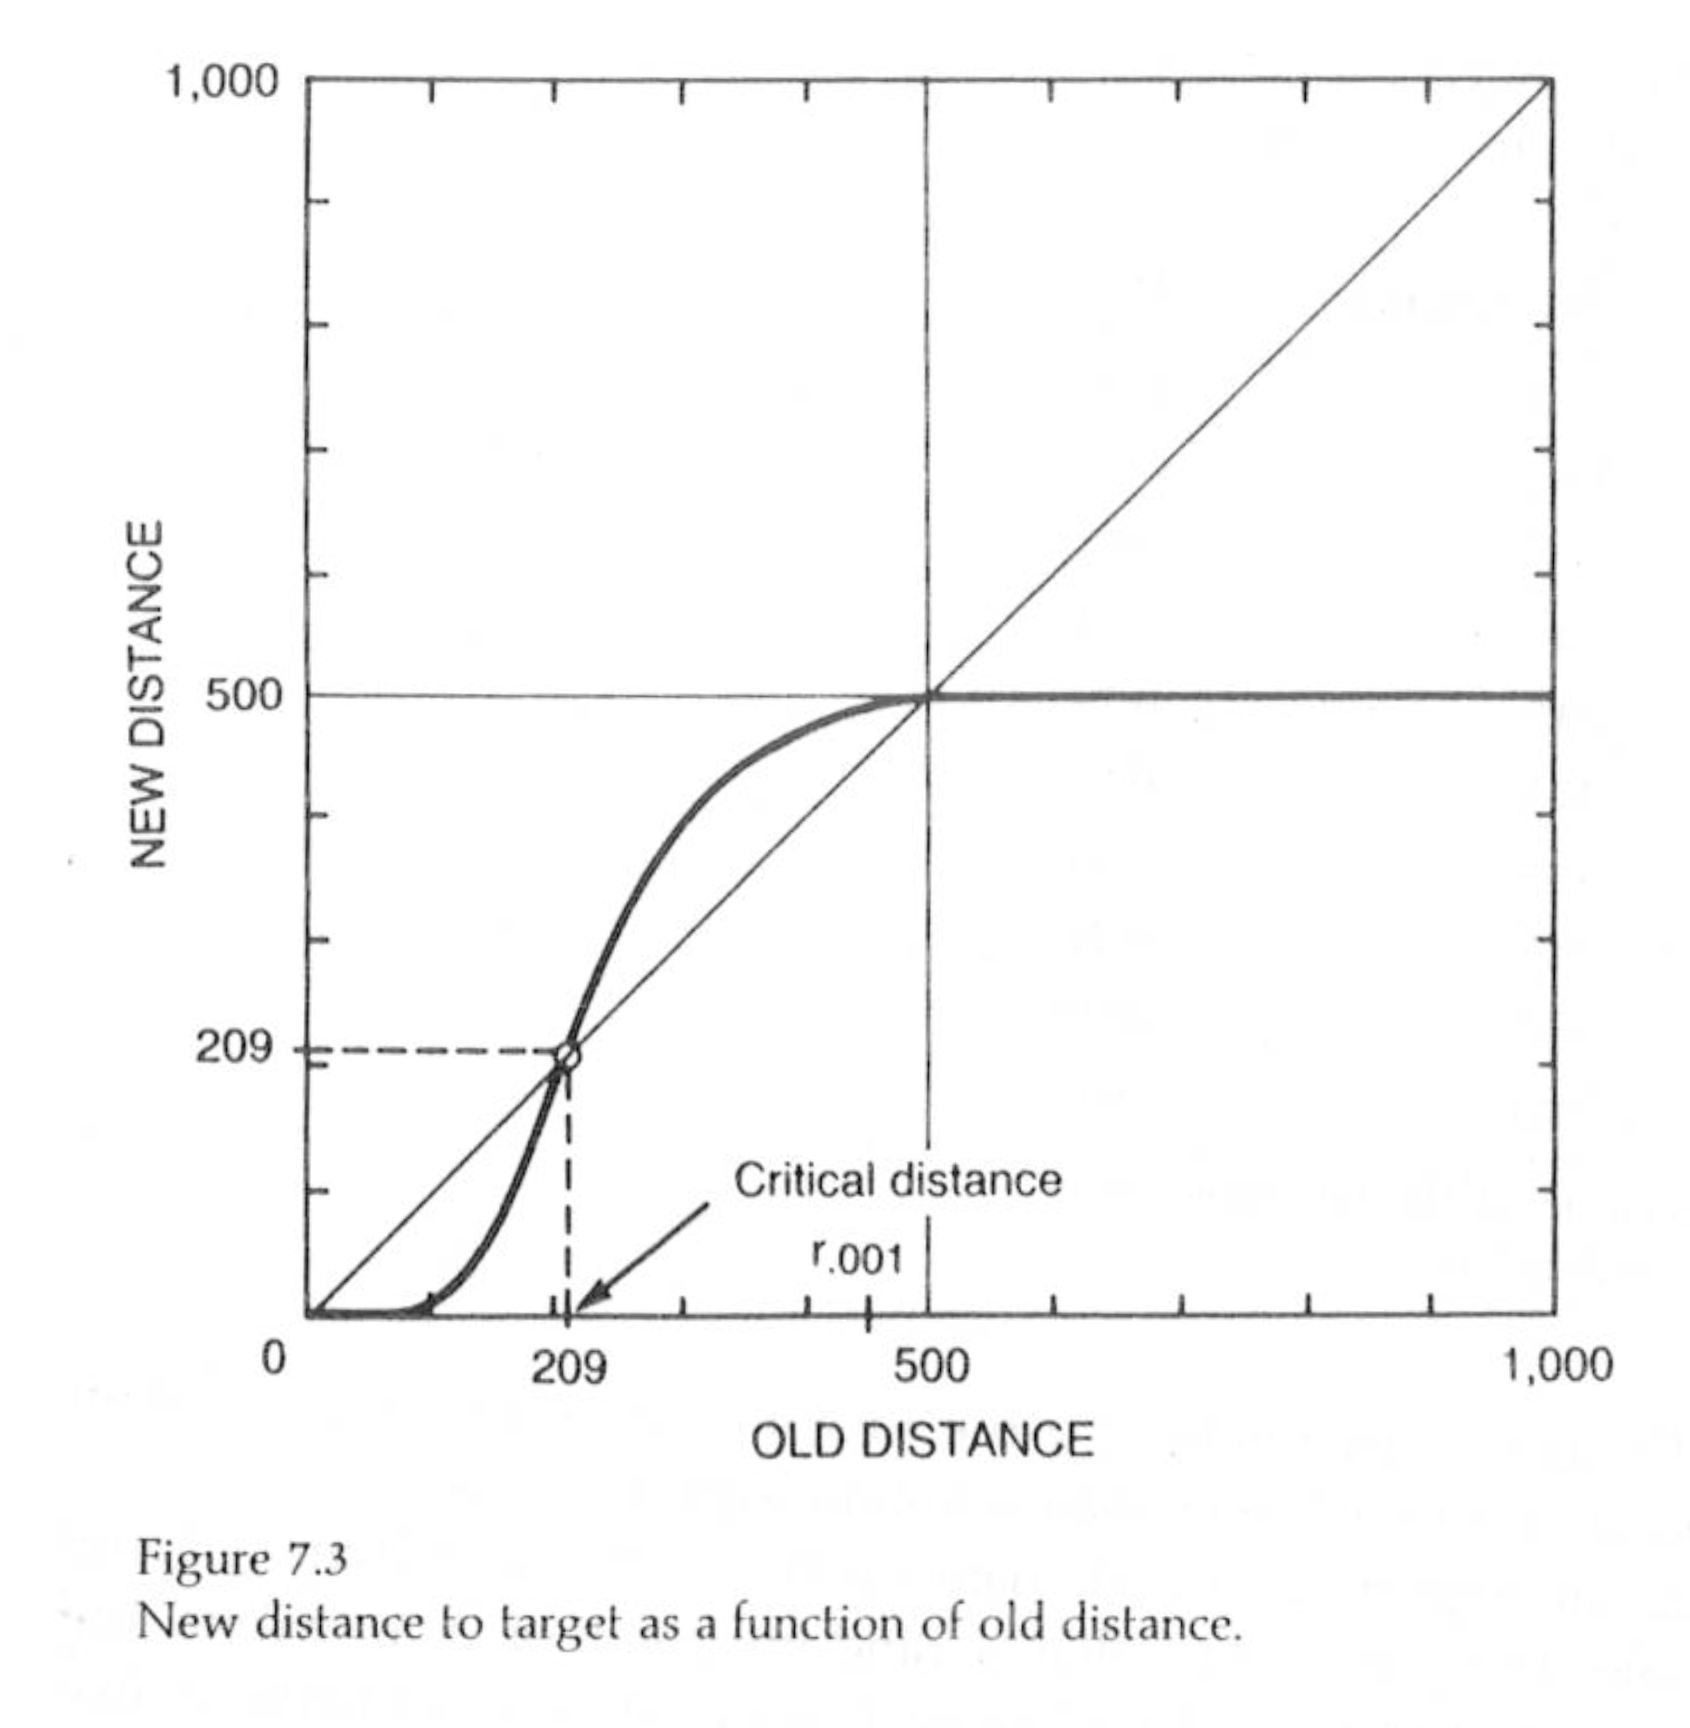
\includegraphics[width=0.8\textwidth]{images02/kanerva-table-7-2-original.png}
\caption{Kanerva's original Figure 7.3 (p. 70) predicting a \textasciitilde 500-bit distance after a point.
\label{fig:kanerva-figure-7.3}}
\end{figure}

As we ran the simulations, this one in particular struck our attention: The new distances obtained after a read operation were not perfectly predicted by the theoretical model.
%and we propose that this is due to interaction effects between different attractors.

We have strictly followed Kanerva's configuration and, even so, we have found out some deviations from Kanerva's original theoretical analysis and the results obtained by simulation.

In details, we have created a SDM with $n=1,000$, $H=1,000,000$, and $r=451$. Then, we have generated 10,000 random bitstrings and written them into the memory. Then, we have generated a reference bitstring (bs\_ref) and written it into the memory. Then, we have executed the following steps with $x$ from 0 to 1,000: (i) copy bs\_ref into a new bitstring; (ii) randomly flipped $x$ bits of the copy; (iii) read from the memory in the copy address; and (iv) stored the distance between the returned bitstring and bs\_ref. Finally, we have plotted Figure \ref{fig:sdm-10000w-table-7-2}.

\begin{figure}[h]
\centering
\subfloat[1 sample for each distance $x$ \label{fig:sdm-10000w-table-7-2-1sample} ]{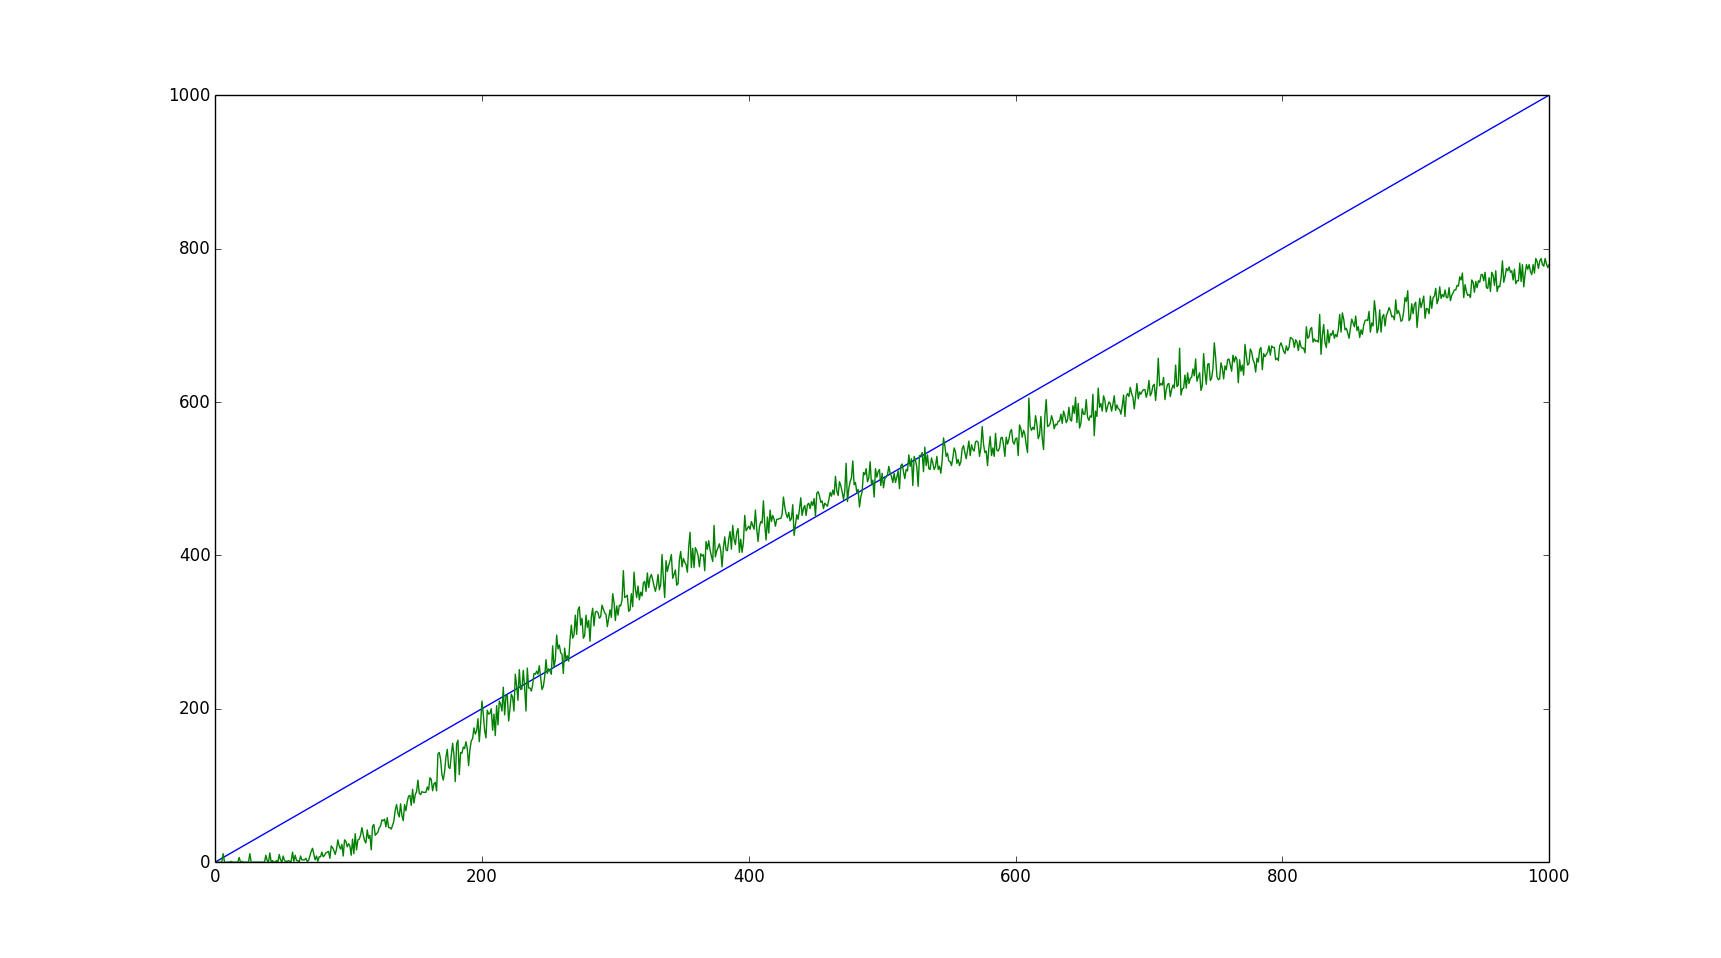
\includegraphics[width=0.5\textwidth]{./images02/sdm-10000w-table-7-2.png}}
\subfloat[6 samples for each distance $x$ \label{fig:sdm-10000w-table-7-2-6samples} ]{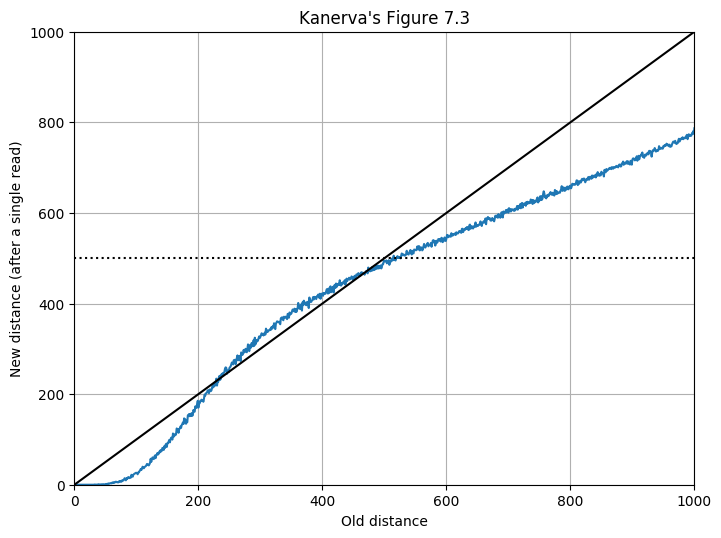
\includegraphics[width=0.5\textwidth]{./images02/sdm-10000w-table-7-2-6-samples.png}}

\caption{Results generated by the framework diverging from Kanerva's original Table 7.2. Here we had a 1,000 bit, 1,000,000 hard-location SDM with exactly 10,000 random bitstrings written into it, which was also Kanerva's configuration.
\label{fig:sdm-10000w-table-7-2}}
\end{figure}

Figure \ref{fig:sdm-10000w-table-7-2-1sample} has a lot of noise because we have read only once for each distance $x$ and Kanerva has predicted the average distance. So, we have changed the steps to run $k$ reads and store the average new distance. We run with $k=6$, and the results can be seen in Figure \ref{fig:sdm-10000w-table-7-2-6samples}, which has a way lower noise and still holds the divergence.

Our results show that the theoretical prediction is not accurate.  There are interaction effects from one or more of the attractors created by the 10,000 writes, and these attractors seem to raise the distance beyond \textasciitilde 500 bits (Figure \ref{fig:sdm-10000w-table-7-2}).

Obviously, these small deviations from Kanerva's original theoretical predictions deserve a qualification.  Kanerva was working in the 1980s and the 1990s, and had no access to the immense computational power that we do today. It is no surprise that some small interaction effects should exist as machines allow us to explore the ideas of his monumental work.

But, when we reduced the number of random bitstrings written in the SDM from 10,000 to only 100, the results reflected very well the Kanerva's theoretical expectation (Figure \ref{fig:sdm-100w-table-7-2-10samples}). This result strengthens our hypothesis that the disparities in the computational results are due to the interaction effect of high numbers of different attractors. In Figure \ref{fig:sdm-table-7-2-steps} we can notice that, the more random bitstrings are written, the stronger the attractots.

\begin{figure}[h]
\centering
\subfloat[100 writes \label{fig:sdm-100w-table-7-2-10samples} ]{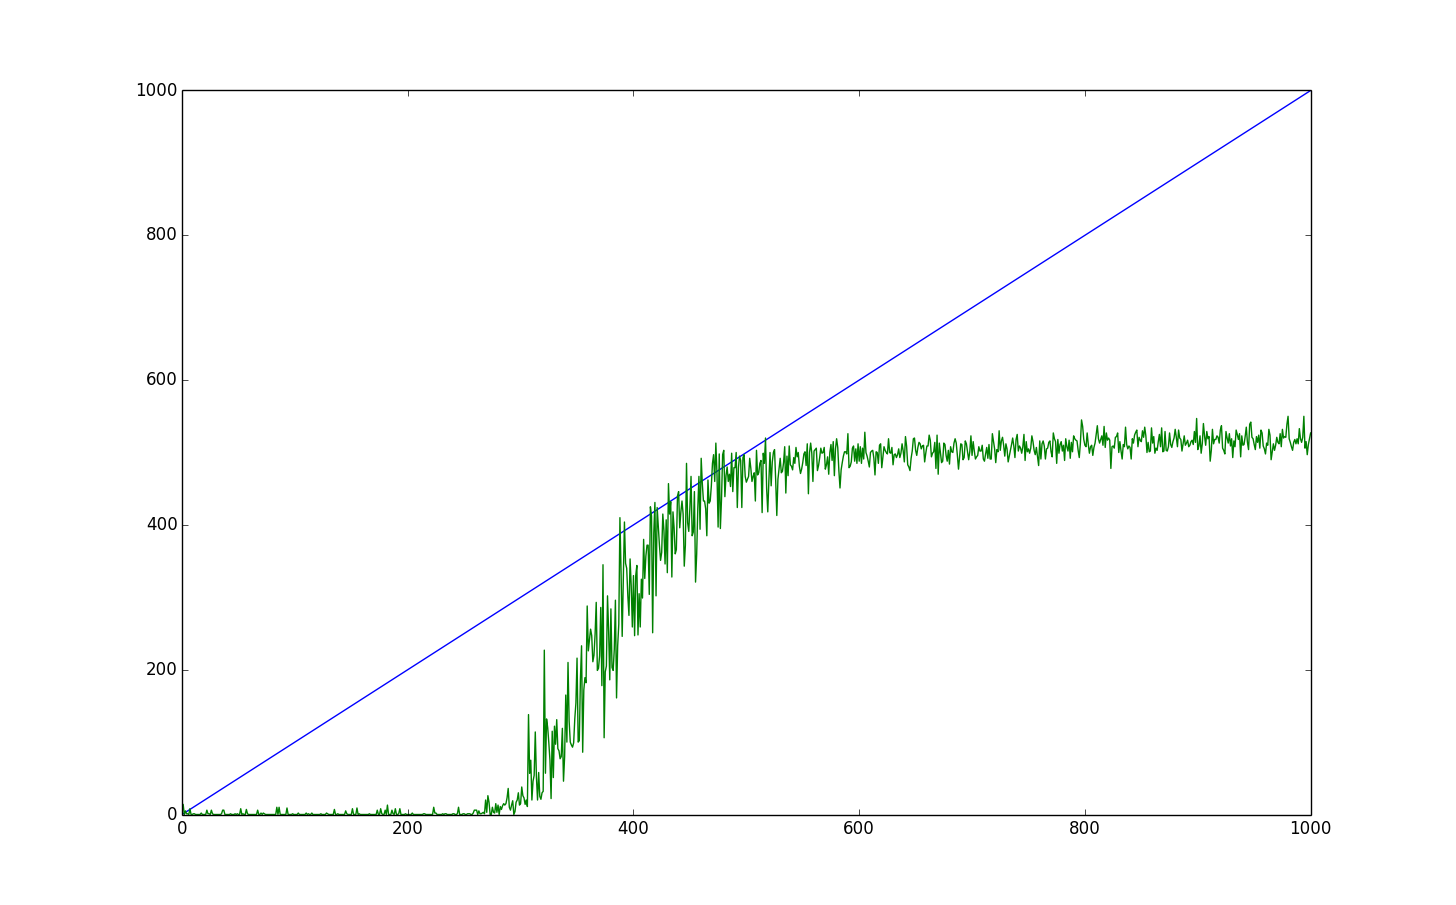
\includegraphics[width=0.47\textwidth]{./images02/sdm-100w-table-7-2.png}}
\subfloat[Steps of 1,000 writes \label{fig:sdm-table-7-2-steps} ]{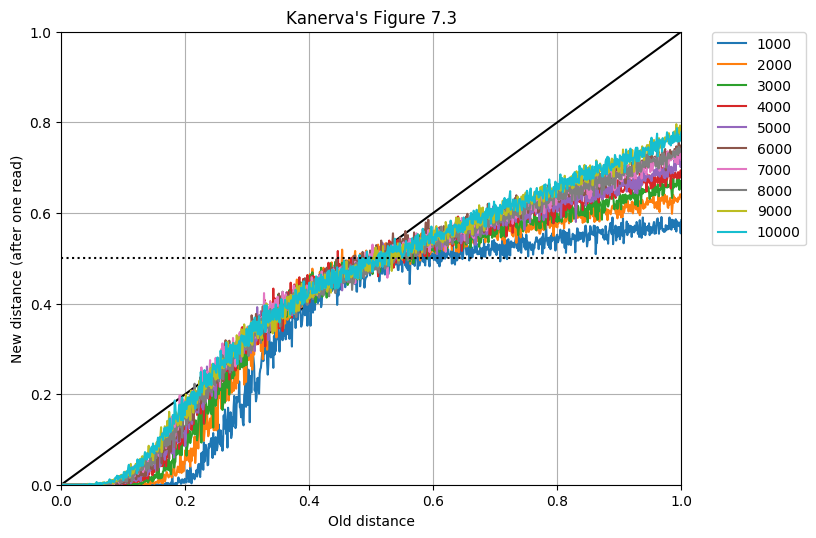
\includegraphics[width=0.53\textwidth]{./images02/sdm-table-7-2-steps.png}}
%\centering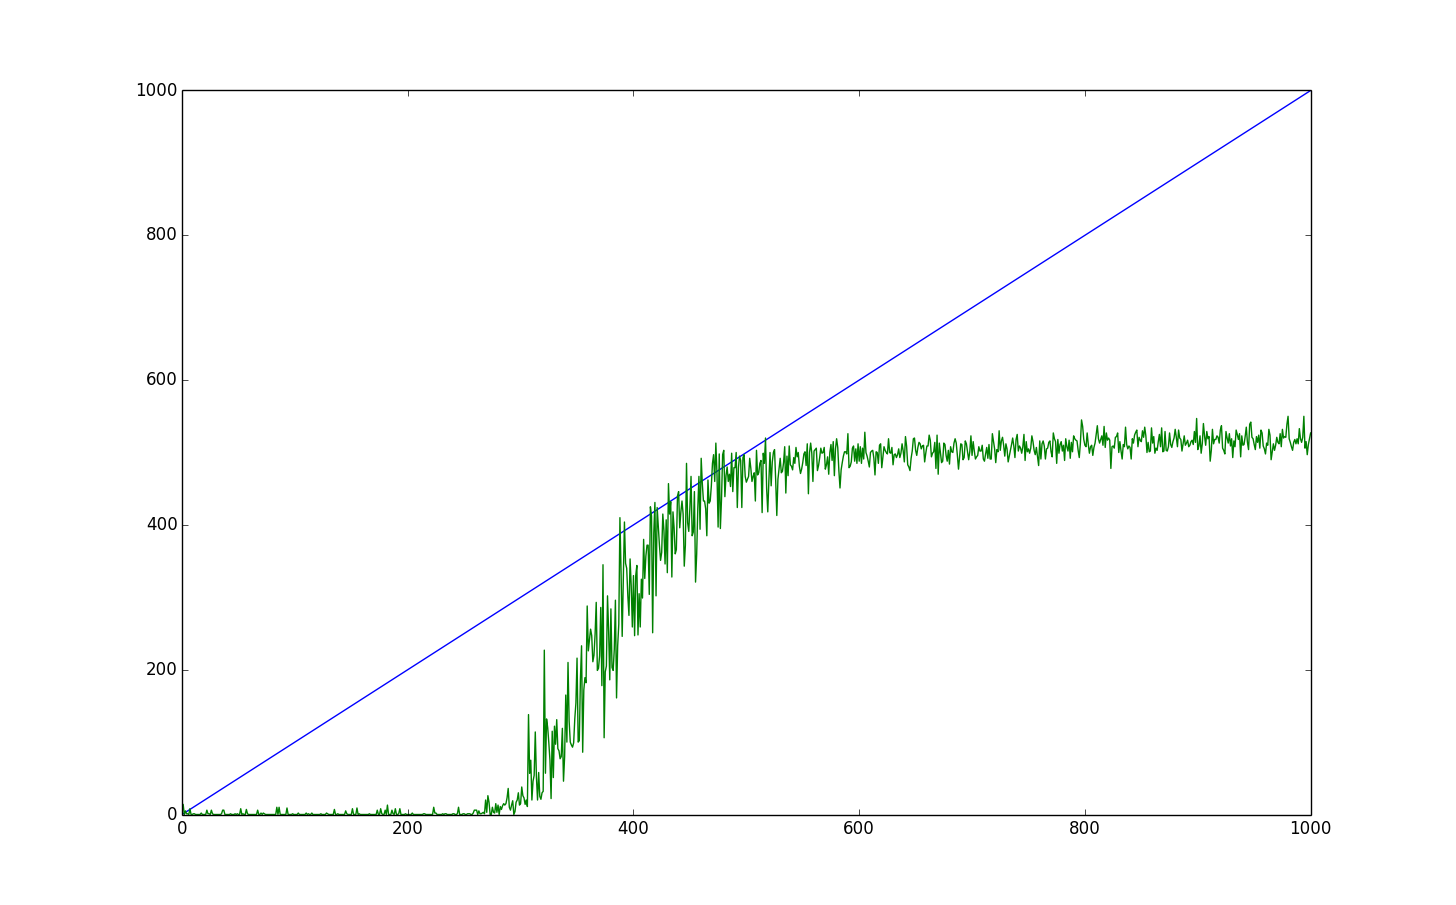
\includegraphics[width=\textwidth]{images02/sdm-100w-table-7-2.png}

\caption{Results generated by the framework similar from Kanerva's original Table 7.2. Here we have a 1,000 bit, 1,000,000 hard-location SDM with (a) exactly 100 random bitstrings written into it and (b) steps of 1,000 random bitstrings written into it.
\label{fig:sdm-100w-table-7-2}}
\end{figure}

To obtain the results from Figures \ref{fig:sdm-10000w-table-7-2} and \ref{fig:sdm-100w-table-7-2}, we had to write 10,000 random bitstrings to an SDM, and then randomly choose one of those bitstrings to be our origin. Finally, we randomly flipped some bits from the origin bitstring and executed a reading operation in the SDM. Thereby, in order to show the interaction effects more clearly, we changed the single read for an 15-iterative read. As we can see in Figure \ref{sdm-10000w-table-7-2-15iter}, after a distance of 500 bits, all bitstrings converged to 500-bit distance bitstrings, just as described by Kanerva.

Hence, our understanding is that the attractors are just preventing the bitstrings to converge directly to 500-bit distance bitstrings, requiring more reading steps to do so. They are in other orthogonal bitstrings' critical distance, but sufficiently far not to converge in a single read.

\begin{figure}[h]
\centering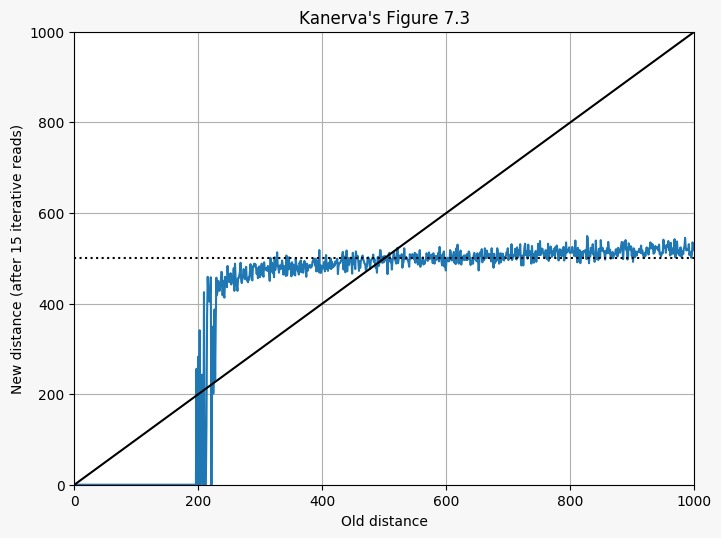
\includegraphics[width=\textwidth]{images02/sdm-10000w-table-7-2-15iter.png}
\caption{This graph shows the interaction effects more clearly.  As we change the single read to a 6-iterative read, the effect has vanished and all bitstrings above $x=500$ have converged to 500-bit distance bitstrings. Here we have the exact same configuration of Figure \ref{sdm-10000w-table-7-2}, except for the iterative read.
\label{sdm-10000w-table-7-2-15iter}}
\end{figure}

%To obtain the results from Figures \ref{fig:sdm-10000w-table-7-2} and \ref{fig:sdm-100w-table-7-2}, we had to write 10,000 random bitstrings to an SDM, and then randomly choose one of those bitstrings to be our origin. Finally, we randomly flipped some bits from the origin bitstring and executed a reading operation in the SDM. Thereby, in order to show the interaction effects more clearly, we wrote a handmade bitstring to the SDM which had all bits inverted in relation to the origin bitstring --- their hamming distance was equal to 1,000. Our handmade bitstring was acting as an opposite attractor, and one can see the accelerating effects towards convergence to both attractors: the origin and the handmade bitstrings (Fig. \ref{sdm-10000w-notX-table-7-2}). Here we had the exact same configuration of Figure \ref{sdm-10000w-table-7-2}, with the addition of the single opposite attractor.

%\begin{figure}[h]
%\centering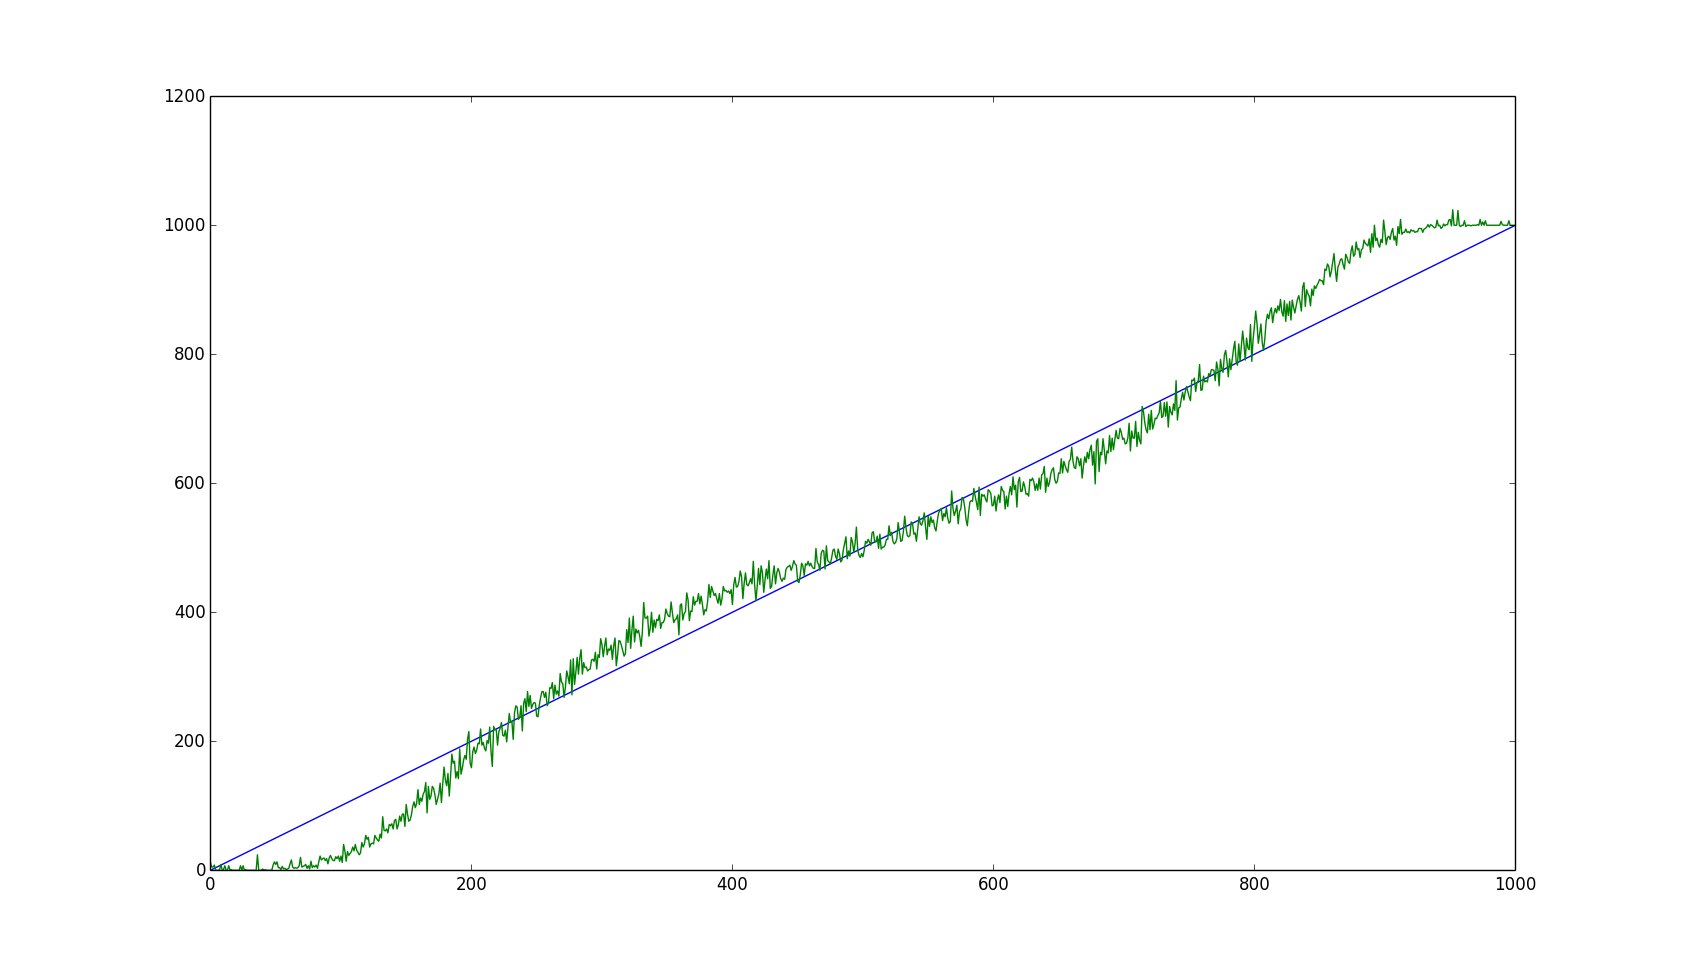
\includegraphics[width=0.8\textwidth]{images02/sdm-10000w-notX-table-7-2.png}
%\caption{This graph shows the interaction effects more clearly.  As we include an opposite bitstring, one can see the accelerating effects towards convergence to both attractors: the origin and the opposite. Here we have the exact same configuration of Figure \ref{sdm-10000w-table-7-2}, with the addition of the single opposite attractor.
%\label{sdm-10000w-notX-table-7-2}}
%\end{figure}



\chapter{Results (ii): Loss of neurons}

In SDM, the data is written distributed among millions of hard-locations, which gives SDM robustness against loss of neurons. In other words, SDM should keep convering correctly even when some neurons are dead. The question is: how robust it really is? How many neurons may die before it starts to forget things.

Looking for answers to those questions, we run a simulation in which we kept killing some neurons and checking whether SDM remained converging to a given bitstring. In this simulation, 10,000 random bitstrings were written to a 1,000-bit SDM.

When we say that we killed a neuron, it means that its hard-location's counters have been zeroed and a new random bitstring address has been given to its hard-location. As no other bitstring is written into the memory, it is exactly like ignoring this hard-location in the next reading operations, i.e., the hard-location does not affect the next reading.

In Figure \ref{fig:sdm-neuron-death-50k}, we can notice that SDM is absolutely robust up to 50,000 neuron deaths which is 5\% of the all hard-locations.

\begin{figure}[h]
\centering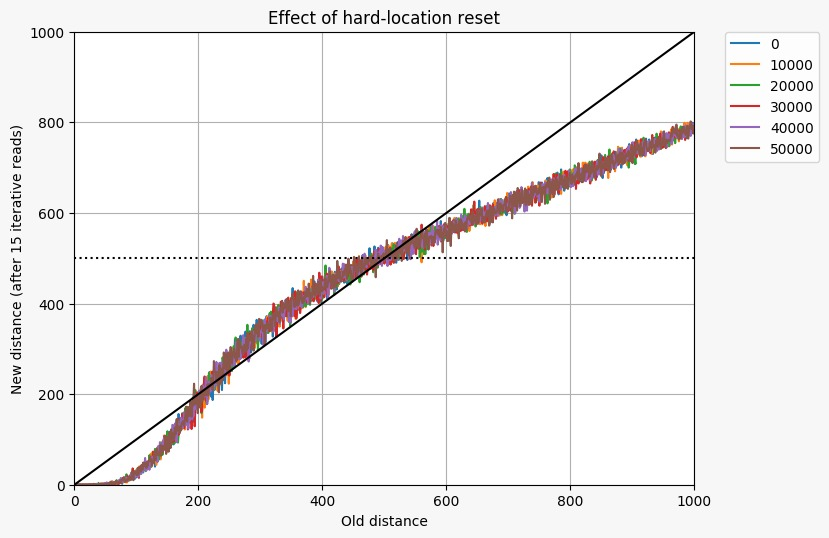
\includegraphics[width=\textwidth]{./images02/new-images/sdm-neuron-death-50k.png}
\caption{This graph shows the SDM's robustness against loss of neurons. It shows from 0 to 50,000 neuron deaths.
\label{fig:sdm-neuron-death-50k}}
\end{figure}

In fact, SDM begins to be affected by loss of neurons after 600,000 deaths (Figure \ref{fig:sdm-neuron-death-1m}), and obviously forgets everything when all neurons are dead.

It is interesting that 500,000 deaths have almost no effect in SDM's recall. It is analogous to do an hemispherectomy in a person and, after the procedure, the person is able to recall exactly like before.

\begin{figure}[h]
\centering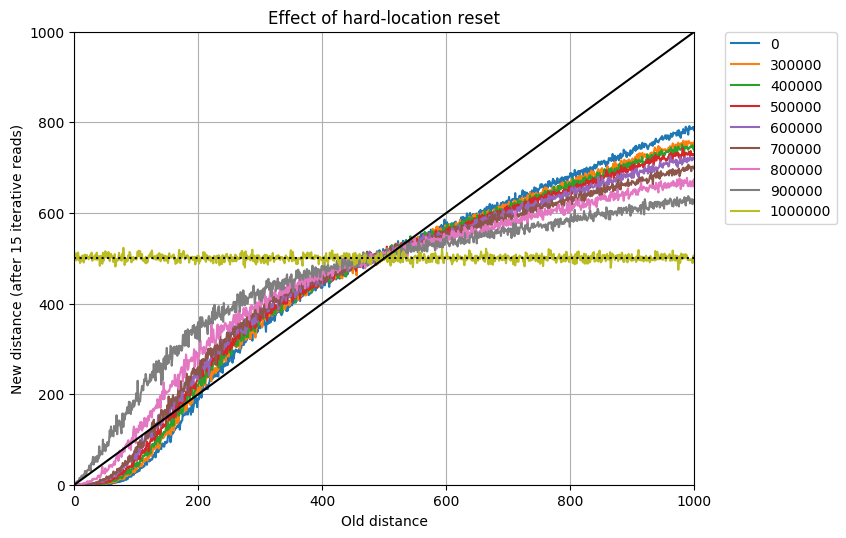
\includegraphics[width=\textwidth]{./images02/new-images/sdm-neuron-death-1m.png}
\caption{This graph shows the SDM's robustness against loss of neurons.
\label{fig:sdm-neuron-death-1m}}
\end{figure}

Although there is some decrease in SDM after 600,000, it is curious that there is a sudden change between 900,000 (90\%) and 1,000,000 (100\%). In Figure \ref{fig:sdm-neuron-death-details} we can see the details of this non-linear change.

\begin{figure}[h]
\centering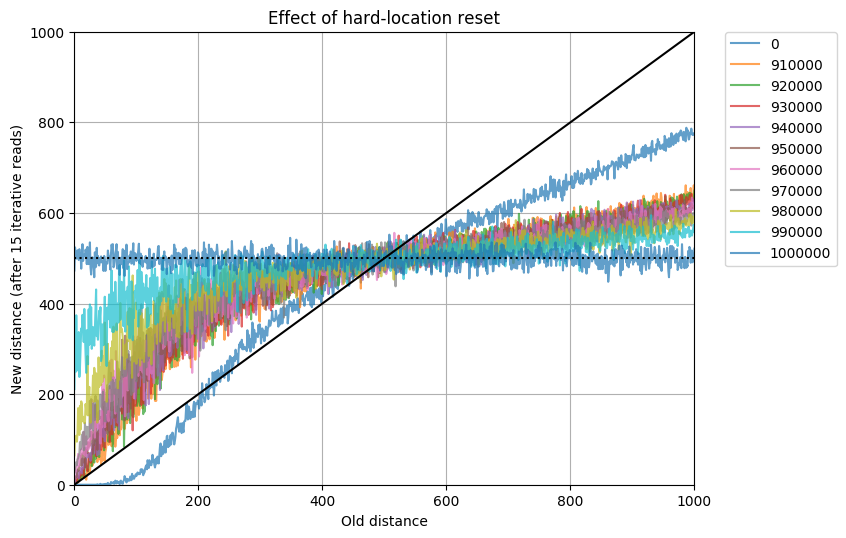
\includegraphics[width=\textwidth]{images02/new-images/sdm-neuron-death.png}
\caption{This graph shows the SDM's robustness against loss of neurons. In each color, a given amount of neurons have been killed.
\label{fig:sdm-neuron-death-details}}
\end{figure}


\chapter{Results (iii): Generalized read operation}

In this chapter we will explore how the generalized read operation works and whether it may improve SDM behavior. In this case, we understand that SDM behavior will have been improved when the critical distance increases, which means it is able to recognize things with even less clues than before.

In Figure

\begin{figure}[h!]
  \centering
  \subfloat[SDM behavior when $z \in \{0.1, 0.2, 0.3, 0.4, 0.5, 1\}$ ]{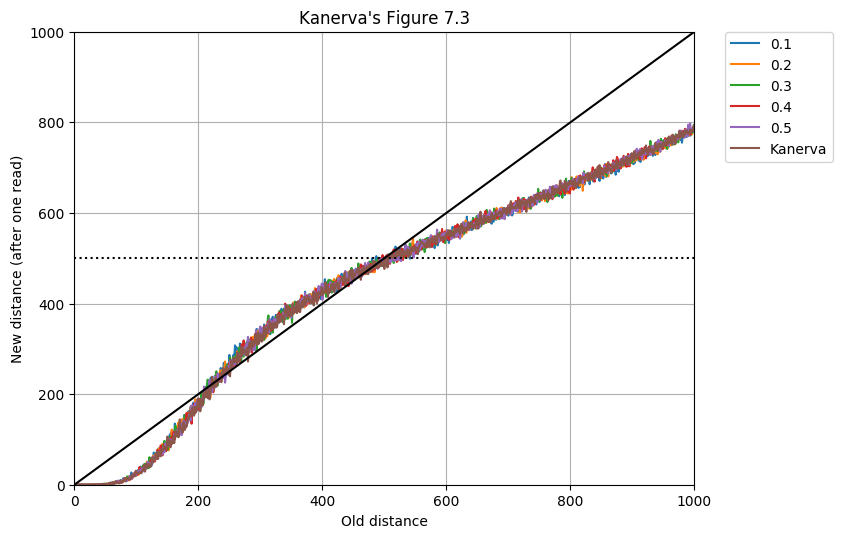
\includegraphics[width=\textwidth]{./images02/new-images/iter_z_01-05.png}}

  \subfloat[SDM behavior when $z \in \{1.5, 3, 4.5, 6\}$ ]{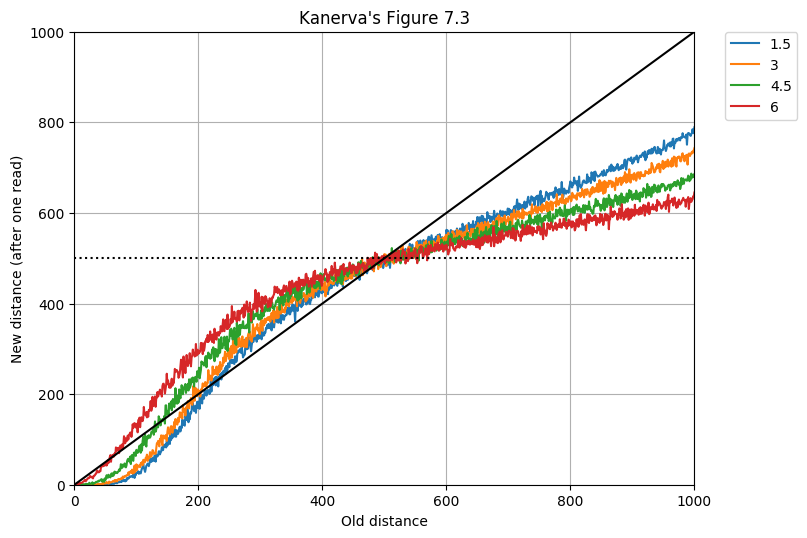
\includegraphics[width=\textwidth]{./images02/new-images/z_15_3_45_6.png}}

  \caption{(a) and (b) show the behavior of a single read; As stated previously, we can see a deterioration of convergence, with lower critical distance as $z>1$.  Another observation can be made here, concerning the discrepancy of Kanerva's Fig 7.3 and our data.  It seems that Kanerva may not have considered that a single read would only `clean' a small number of dimensions \emph{after the critical distance}. What we observe clearly is that with a single read, as the distance grows, the system only `cleans' towards the orthoghonal distance 500 after a number of iterative readings.}
  \label{fig:murillo-generalization-experiments}
\end{figure}

\begin{figure}[h!]
  \centering
  \subfloat[$z \in \{0, 1\}$]{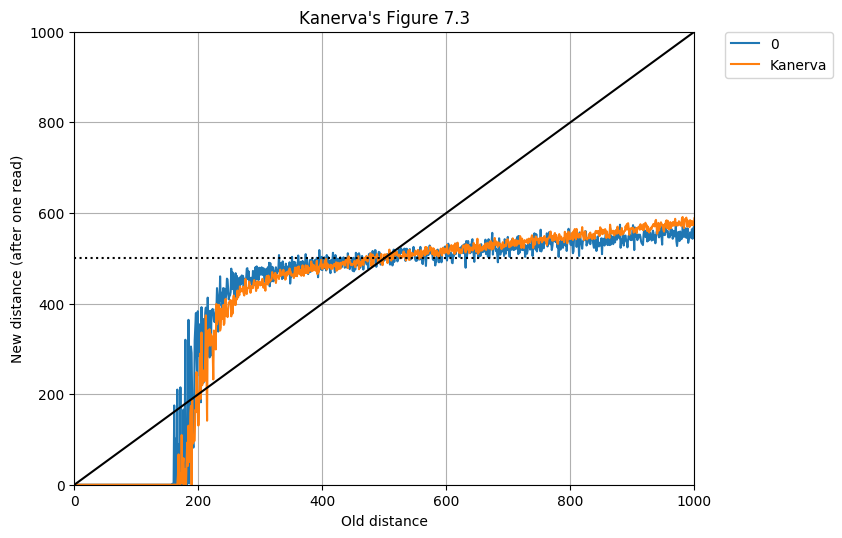
\includegraphics[width=3.2in]{./images02/new-images/z_0_1.png}}

  \subfloat[$z \in \{0, 0.5, 1, 1.5, 3, 4.5, 6\}$]{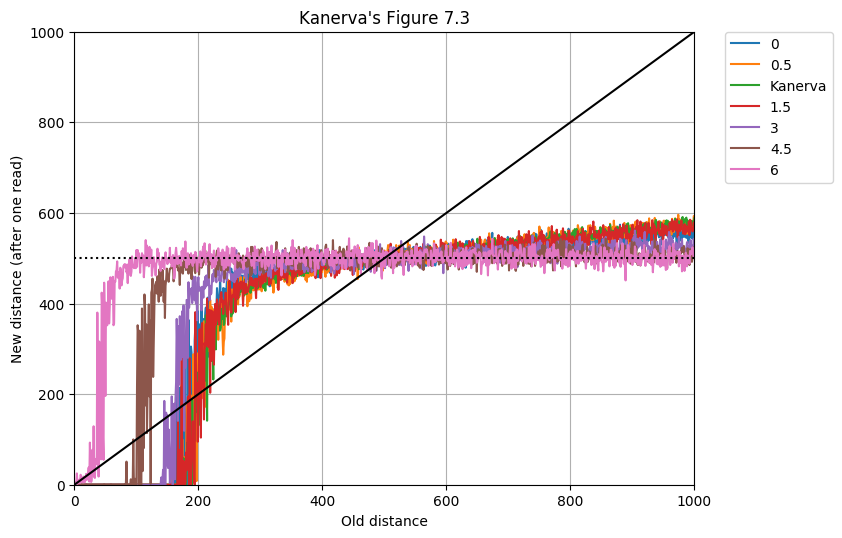
\includegraphics[width=3.2in]{./images02/new-images/iter_z_all_2.png}}

  \caption{(a) and (b) show the behavior of the previous Figure, now executed with 6 iterative reads. What we observe clearly is that with a single read, as the distance grows, the system only `cleans' towards the orthoghonal distance 500 after a number of iterative readings.}
  \label{fig:murillo-generalization-experiments-6reads}
\end{figure}



Physicist Paulo Murilo observed that the models of Kanerva-read ($z=1$) and Chada-read ($z=0$) were simple variations of the exponent $z$, which suggests experimenting with different values. The results, however, have not yielded performance improvements.  Though for $z \leq 1$ results are comparable to $z=1$, for $z>1$, the system shows a clear deterioration, with a smaller distance to convergence and higher divergence at large-distance reads. This is shown in Figures \ref{fig:murillo-generalization-experiments} and \ref{fig:murillo-generalization-experiments-6reads}.


\chapter{Results (iv): Performance}

Our intention is to provide comparative performance metrics under different computation engines (CPU, GPU, etc) and different operating systems (Linux, MacOs, Windows, etc). Performance can be measured as the average number of scans of all hard locations per second, reads per second, writes per second, etc.

Our first device is a personal MacBook Pro Retina 13-inch Late 2013 with a 2.6GHz Intel core i5 processor, 6GB DDR3 RAM, and Intel Iris GPU.  We also intend to test on machines such as the iMac with dedicated GPU, MacPro with dedicated GPU, and personal computers under Linux with dedicated GPUs.

Beyond that, we are running as state-of-the-art devices: (i) an Amazon EC2 p3.xlarge with Intel Xeon E5-2686v4 processor, 61GB DDR3 RAM, and NVIDIA K80 GPU, and (ii) an Amazon EC2 p3.8xlarge with Intel Xeon E5-2686v4 processor, 488GB DDR3 RAM, and 8x NVIDIA K80 GPU.

% !TEX root = ../partial-sdm.tex

\section{Results (iv): Supervised classification application}

Supervised classification problem consists of categorize data into groups after seeing some samples from each group. First, it is presented pieces of data with their categories. The algorithm learns from these data, which is known as learning phase. Then, new pieces of data are presented and the algorithm must classify them into the already known groups. It is named supervised because  the algorithm will not create the groups itself. It will learn the groups from during the learning phase, in which the groups have already been defined and the pieces of data have already been classified into them.

Although this problem has already been studied (REF), our intention here is to show that a pure SDM may also be used to classify data. \citet{fan1997genetic} has used SDM to solve a classification problem, recognizing handwriting letters from images, but he used a mix of genetic algorithm with SDM, which is very different from the original SDM described by \cite{Kanerva1988}. Even though his algorithm has classified properly, we were intrigued whether a pure SDM would also classify successfully.

Hence, we have developed a supervised classification algorithm based on a pure SDM as our main memory. Our goal was to classify noisy images into their respective letters (case sensitive) and numbers. For some examples, see Figure \ref{fig-classification-examples}.

\begin{figure}[!htb]
\centering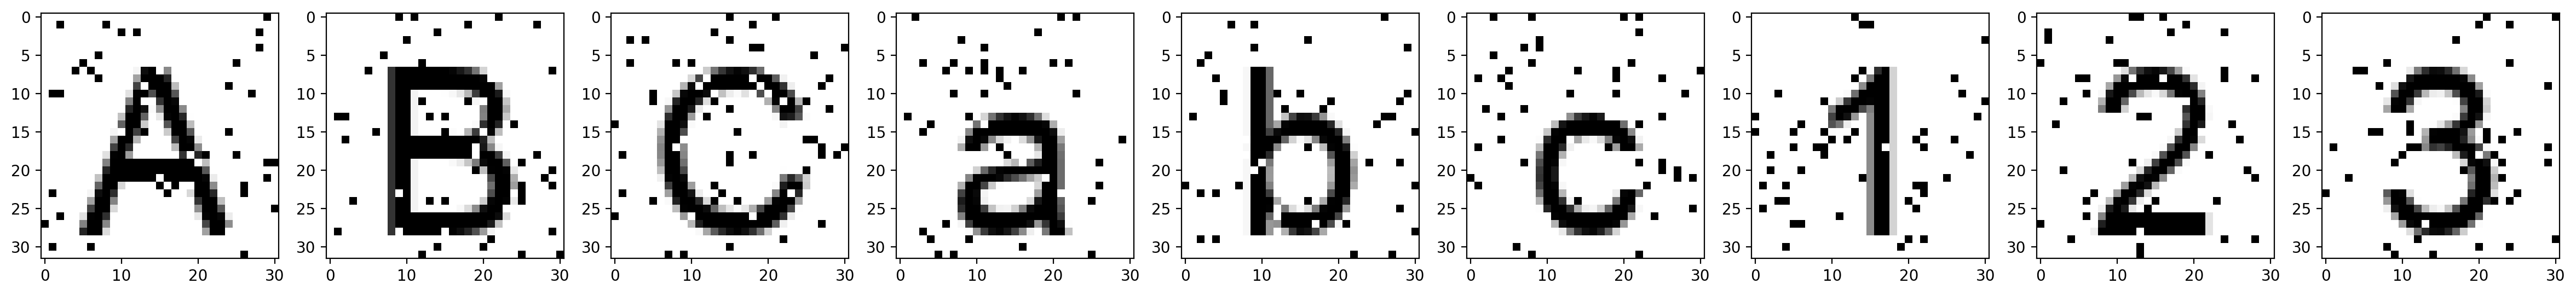
\includegraphics[width=\textwidth]{./images02/classification/example.png}
\caption{Examples of noisy images with uppercase letters, lowercase letters and numbers.
\label{fig-classification-examples}}
\end{figure}

The images had 31 pixels of width and 32 pixels of height, totaling 992 pixels per image. Each image was mapped into a 1,000 bit bitstring in which the bits were set according to the color of each pixel of the image. So, white pixels were equal to bit 0, and black pixels to bit 1. The 8 remaining bits were all set to zero. This was a bijective mapping (or one-to-one mapping), i.e., there was only one bitstring for each image, and there was only one image for each bitstring.

% TODO Add image showing the association between pixels and bits.

A total of 62 classification groups have been trained in the SDM. For each of them, it was generated a random bitstring. Thus, the groups' bitstrings were orthogonal between any two of them. There is one image for each of the 62 groups in Figure \ref{fig-classification-groups}. Notice that the SDM has never seen a single image with no noise.

\begin{figure}[!htb]
\centering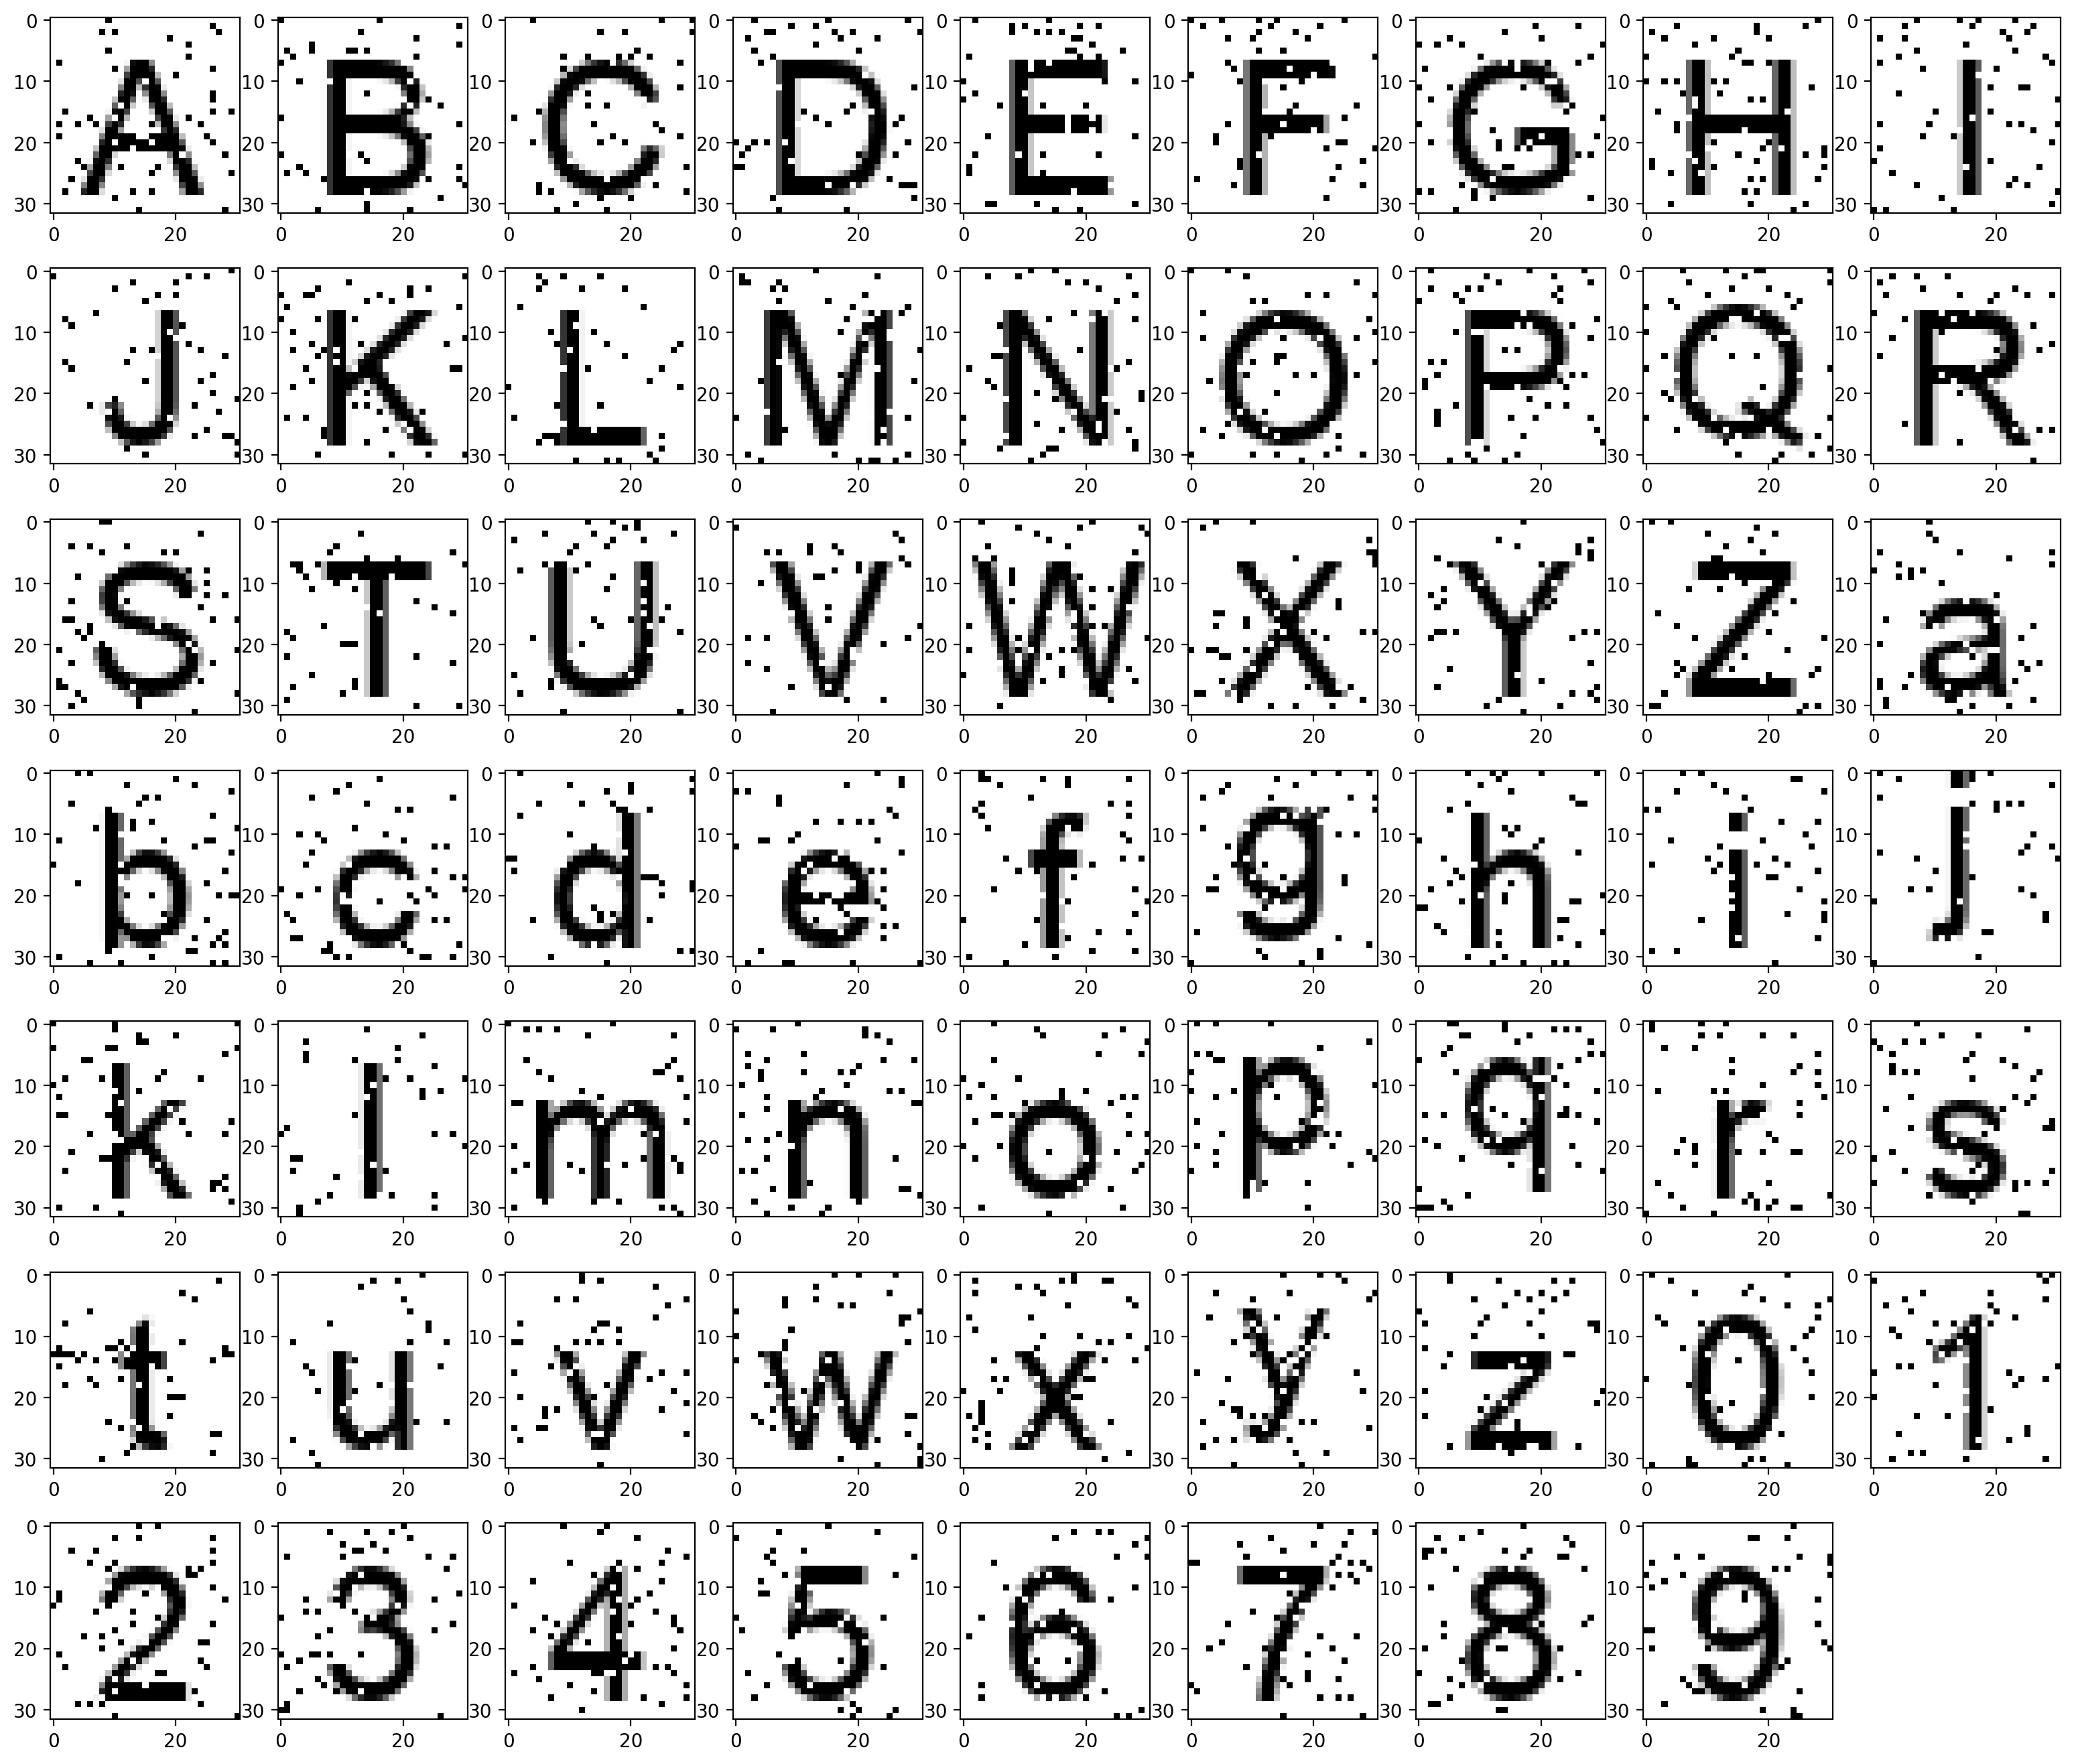
\includegraphics[width=\textwidth]{./images02/classification/groups.png}
\caption{One noisy image for each of the 62 classification groups.
\label{fig-classification-groups}}
\end{figure}

The association of images to groups was stored as sequences in SDM, as detailed by \citet{Kanerva1988} in Chapter 8. During the learning phase, the image bitstrings were stored pointing to their groups bitstrings, i.e., write(addr=bs\_image, datum=bs\_label). Thus, in order to classify an unknown image, we only had to read from its address and check which group has been found.

% TODO Add image showing the pointers.

During the learning phase, we have generated 100 noisy images for each character. The images had 5\% of noise, i.e., 5\% of their pixels have been randomly flipped. For example, see the generated images for letter A in Figure \ref{fig-classification-training-A}. Then, we have wrote the classification group bitstring into the bitstring associated to each noisy image, i.e., write(bs\_image, bs\_label). For a complete image training set, see Appendix XYZ.

\begin{figure}[!htb]
\centering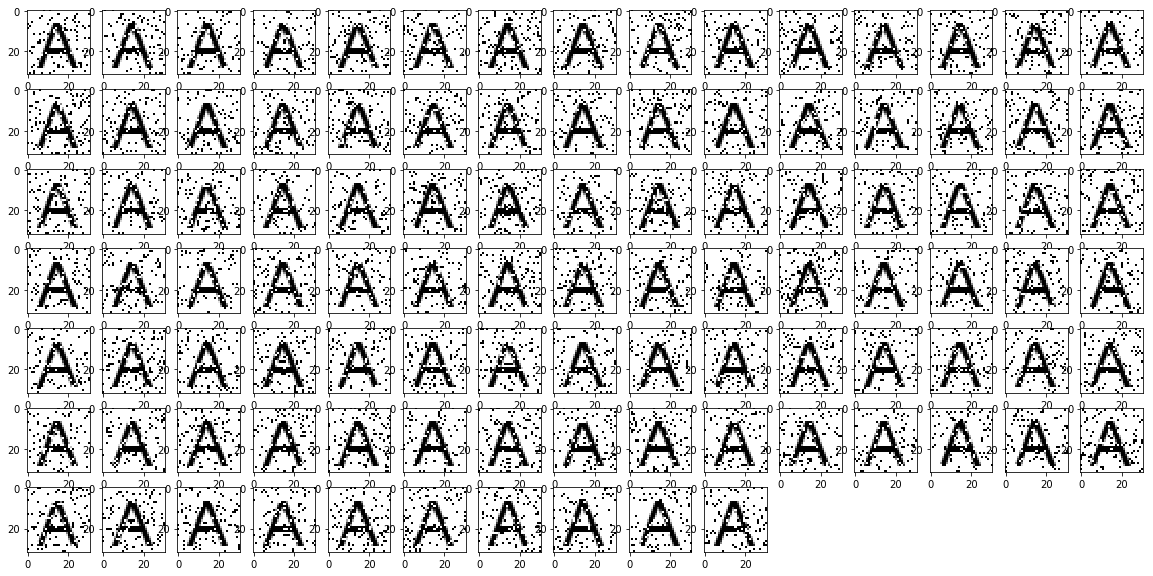
\includegraphics[width=\textwidth]{./images02/classification/trainingA.png}
\caption{100 noisy images generated to train label A.
\label{fig-classification-training-A}}
\end{figure}

Finally, we have assess the performance of our classifier. We had done it in three different scenarios: high noise (20\%), low noise (5\%) and no noise. See Figures \ref{fig-classification-noise-high} and \ref{fig-classification-no-noise} for images with 20\% noise and no noise. The low noise scenario had the same noise as the training set. For each scenario, we had classified 620 unknown images with 10 images per group.

\begin{figure}[!htb]
\centering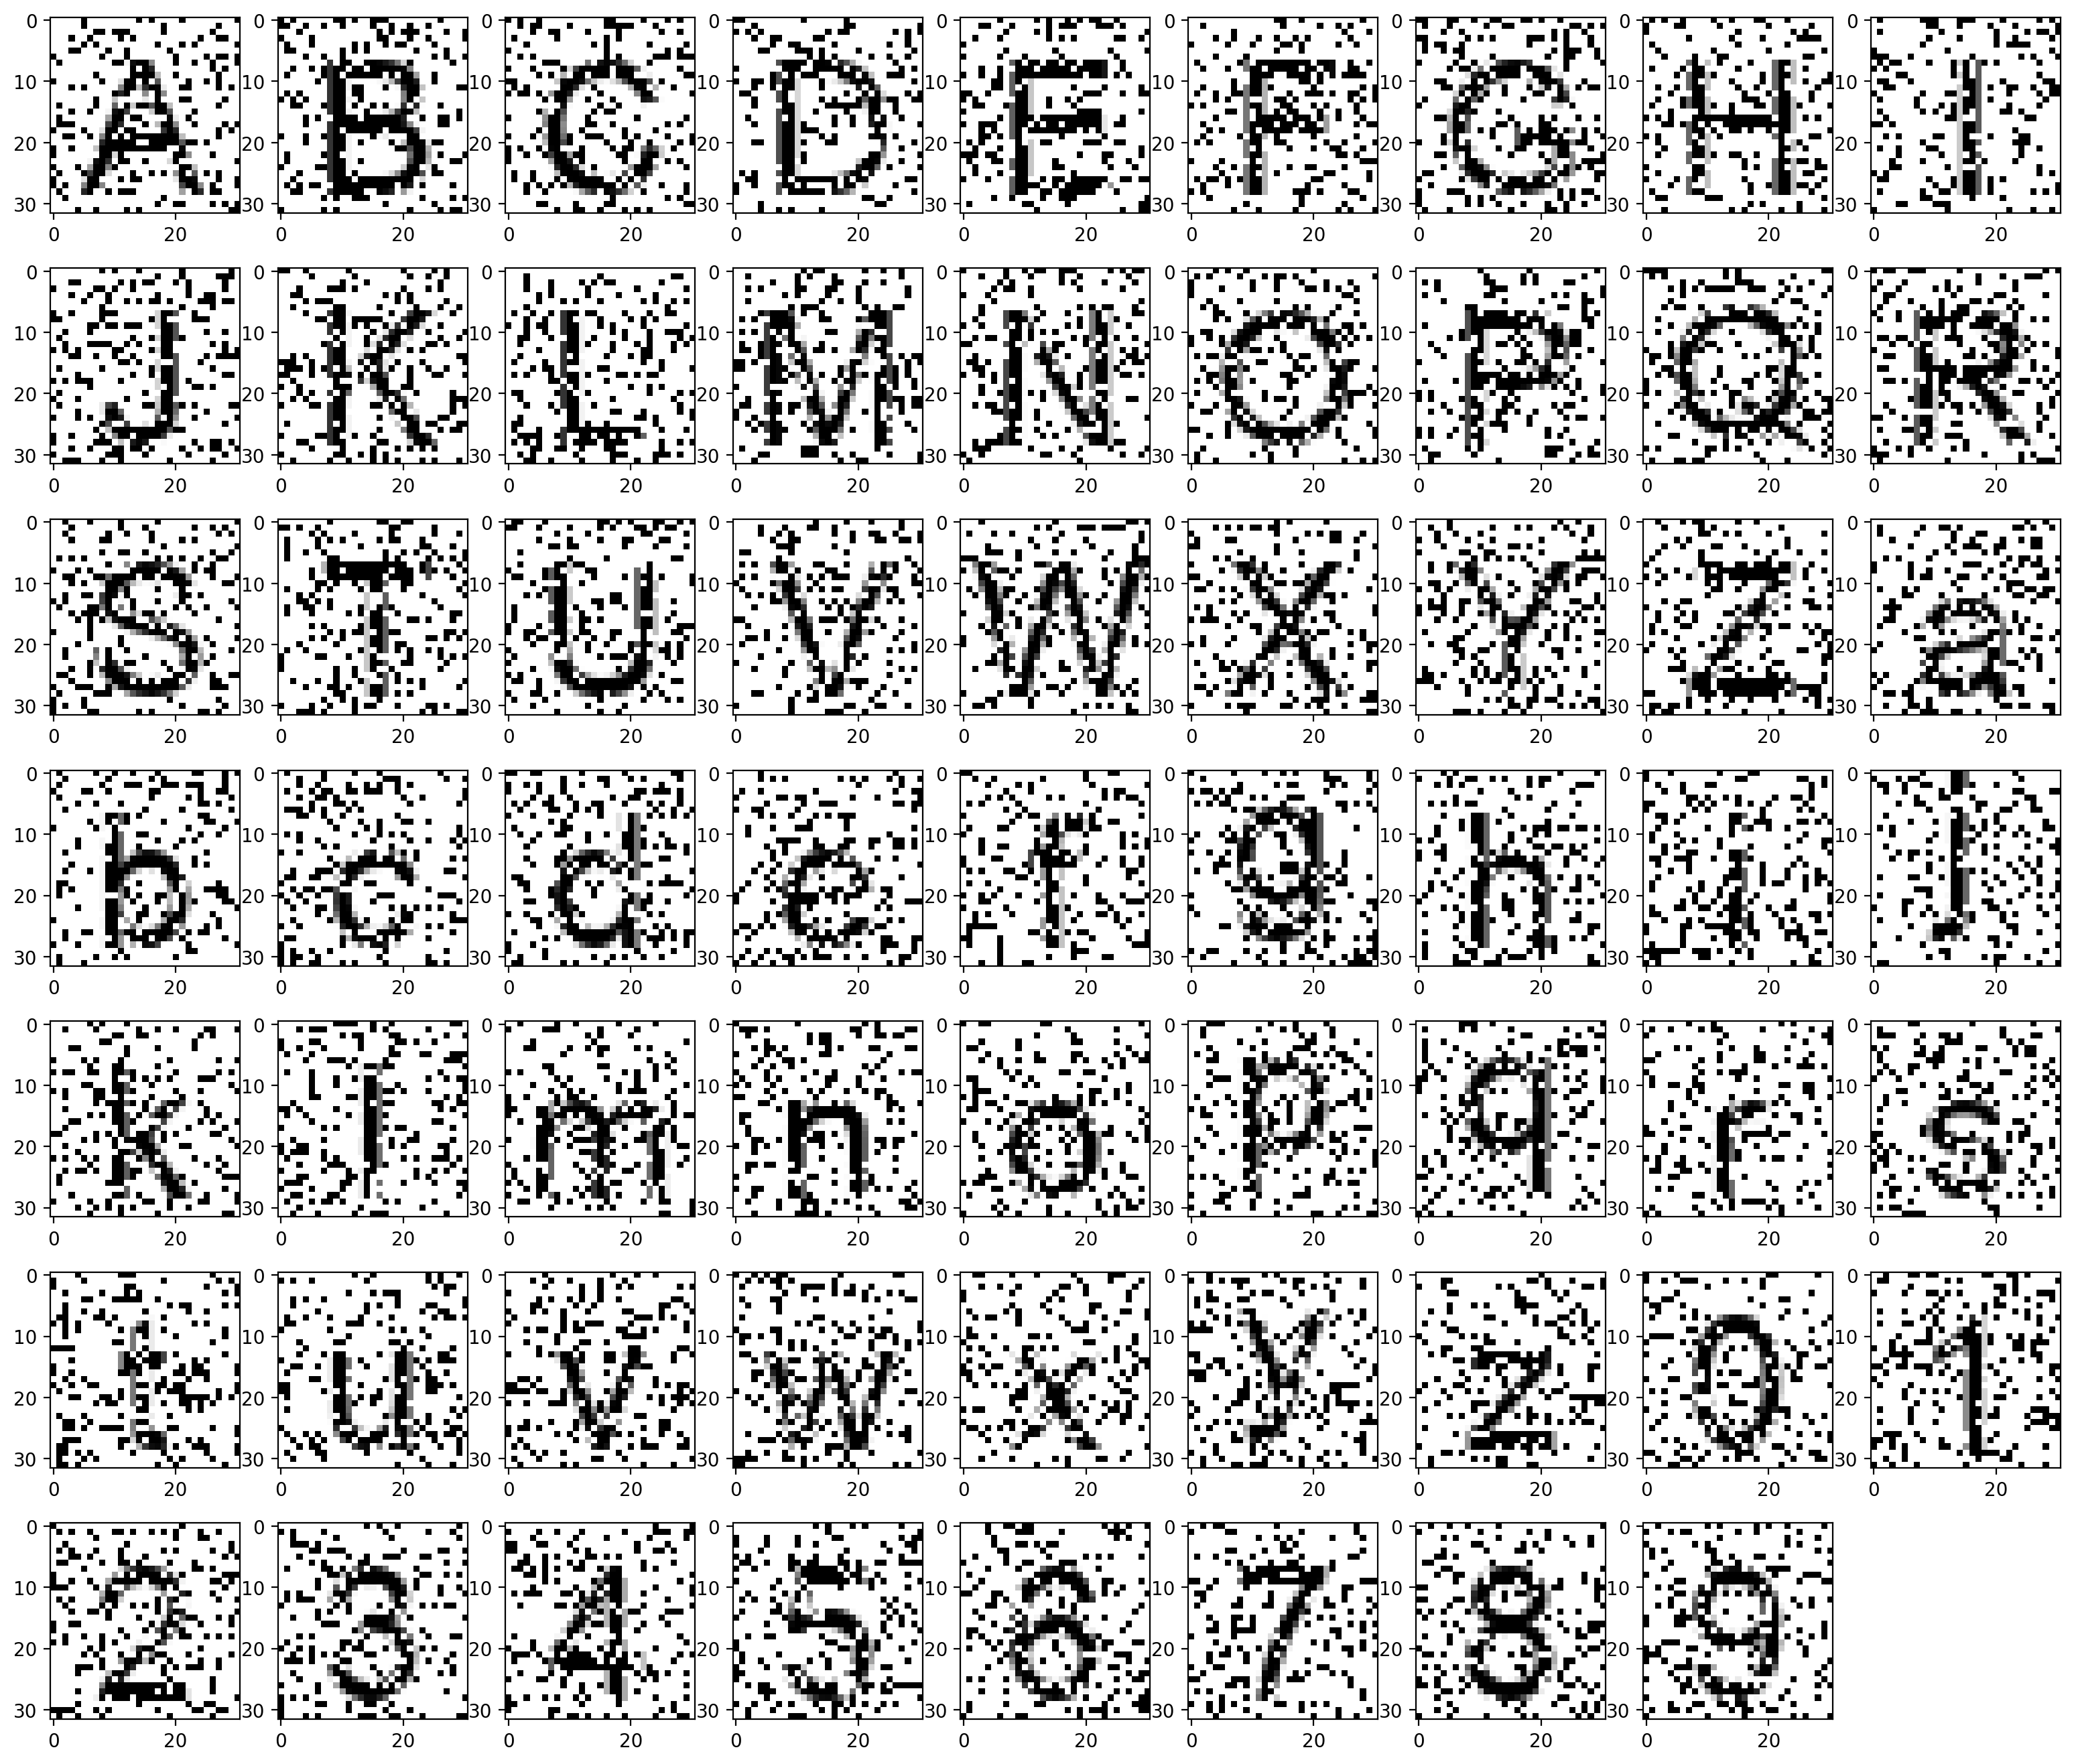
\includegraphics[width=0.75\textwidth]{./images02/classification/noise-high.png}
\caption{Images generated using a 20\% noise for the high noise scenario.
\label{fig-classification-noise-high}}
\end{figure}

\begin{figure}[!htb]
\centering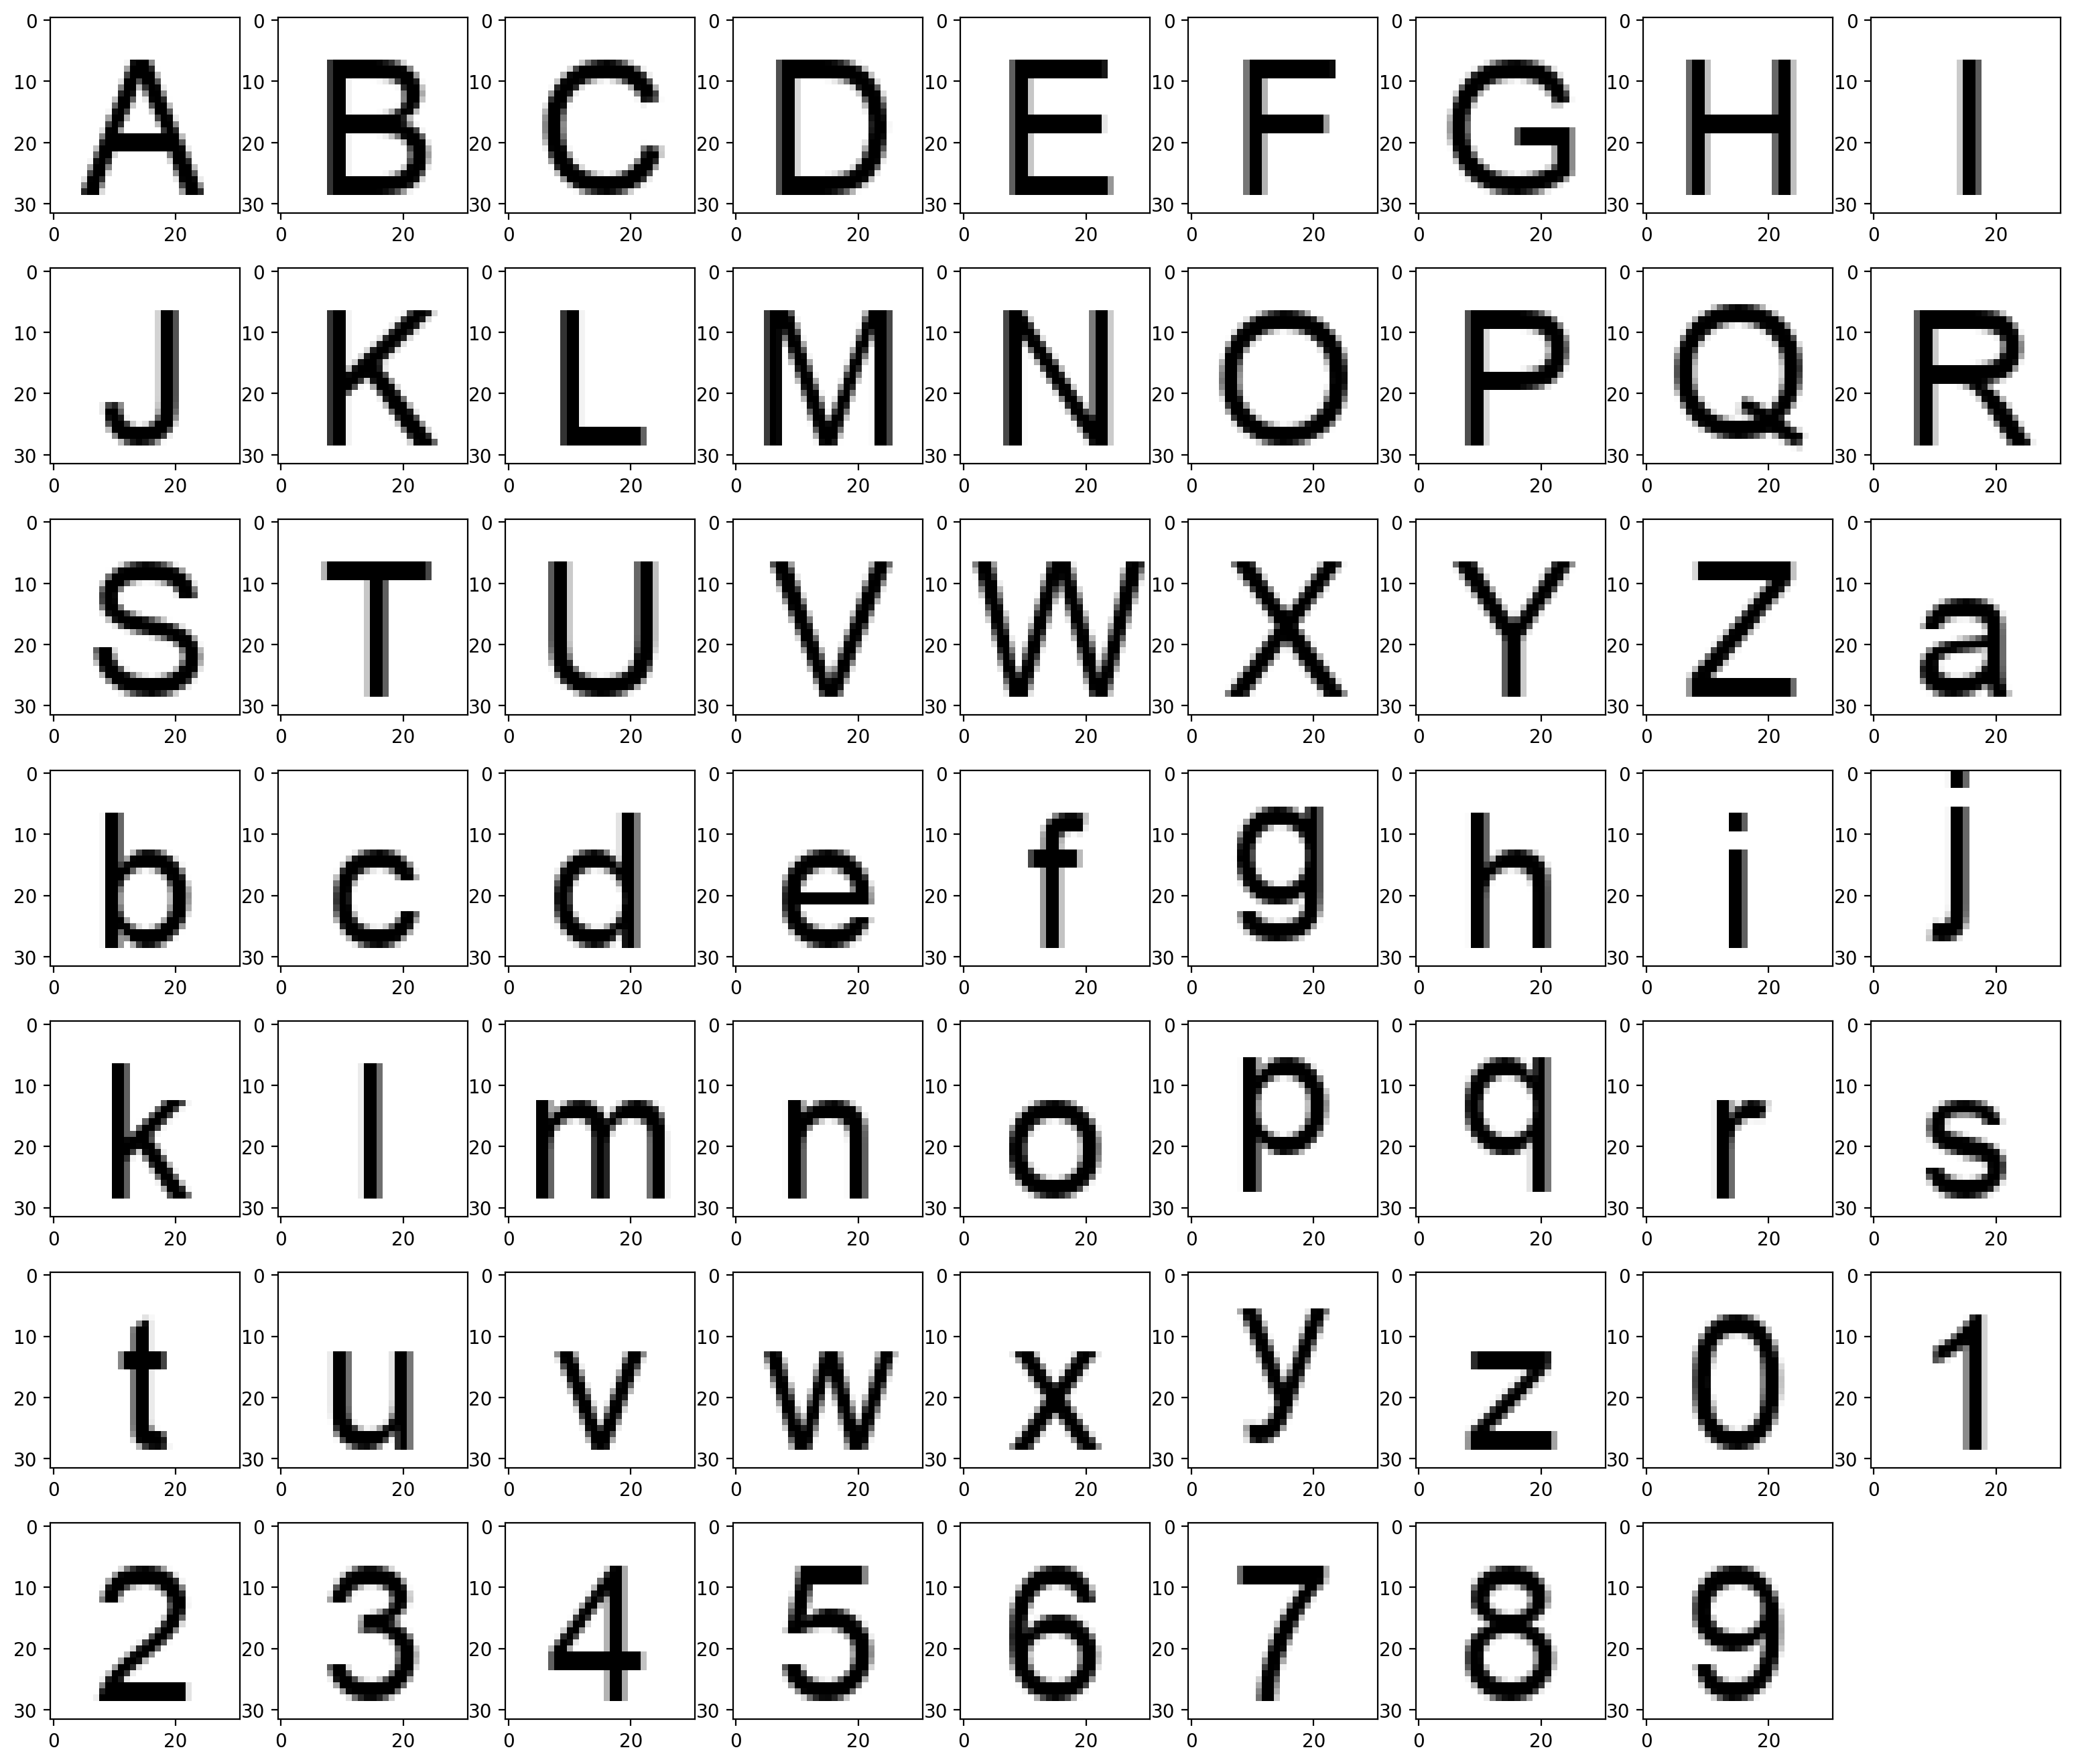
\includegraphics[width=0.75\textwidth]{./images02/classification/no-noise.png}
\caption{Images generated for the no noise scenario.
\label{fig-classification-no-noise}}
\end{figure}

The performance was calculated as the percentage of hits for each group. We did not expected the same performance for all groups because some groups become very similar to other depending on the noise level, and this similarity may even confuse a person (see Figure \ref{fig-classification-similarity}).

\begin{figure}[!htb]
  \centering
  \subfloat[``i'', ``l'', and ``r'' with 20\% noise.]{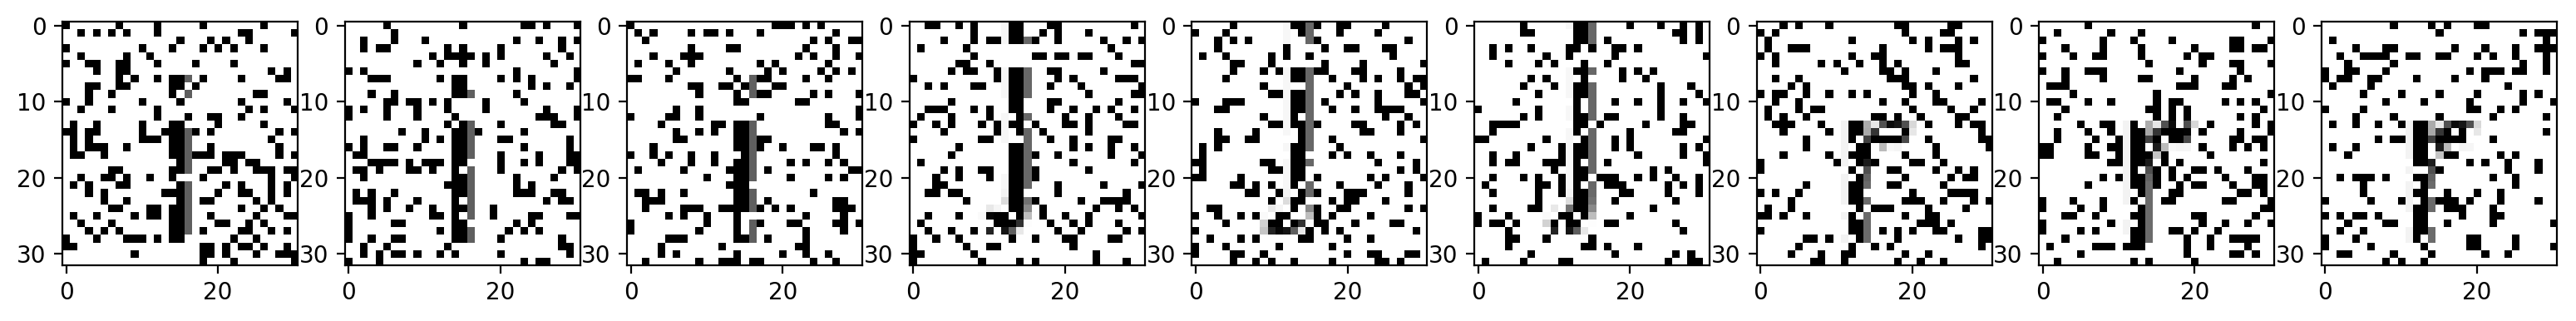
\includegraphics[width=\textwidth]{./images02/classification/ilr-high-noise.png}}

  \subfloat[``i'', ``l'', and ``r'' with 5\% noise.]{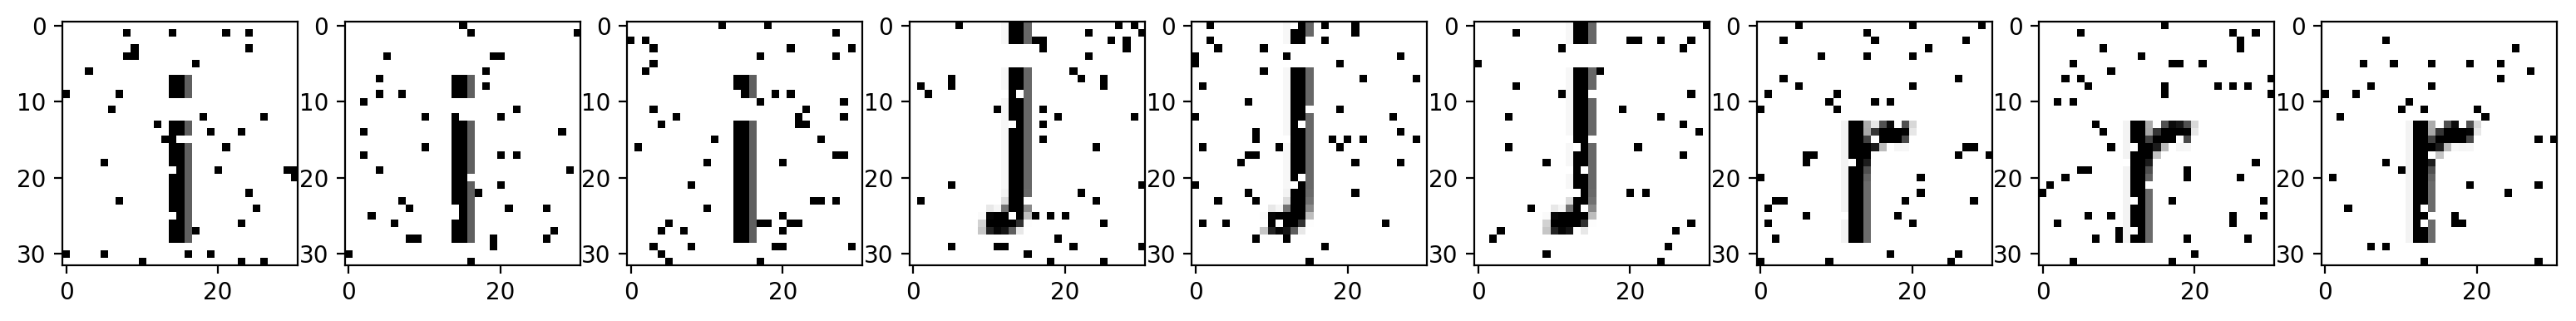
\includegraphics[width=\textwidth]{./images02/classification/ilr-low-noise.png}}

  \subfloat[``c'', ``d'', and ``o'' with 20\% noise.]{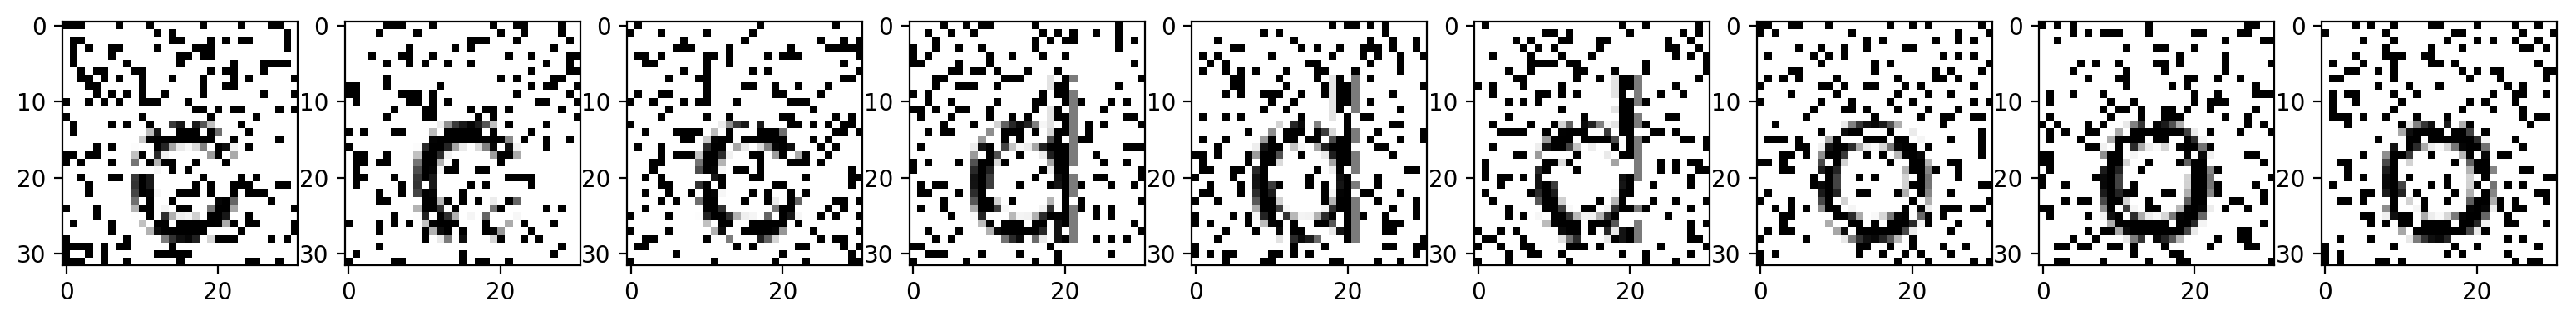
\includegraphics[width=\textwidth]{./images02/classification/cdo-high-noise.png}}

  \subfloat[``c'', ``d'', and ``o'' with 5\% noise.]{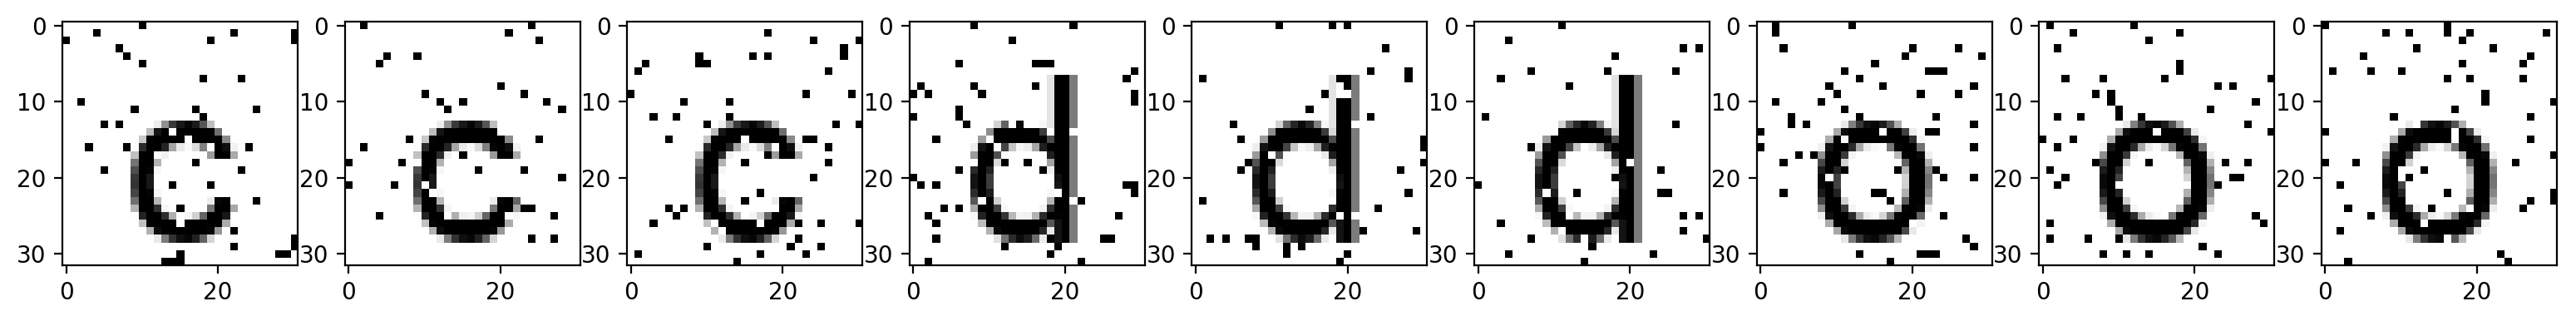
\includegraphics[width=\textwidth]{./images02/classification/cdo-low-noise.png}}

  \subfloat[``G'', ``O'', and ``Q'' with 20\% noise.]{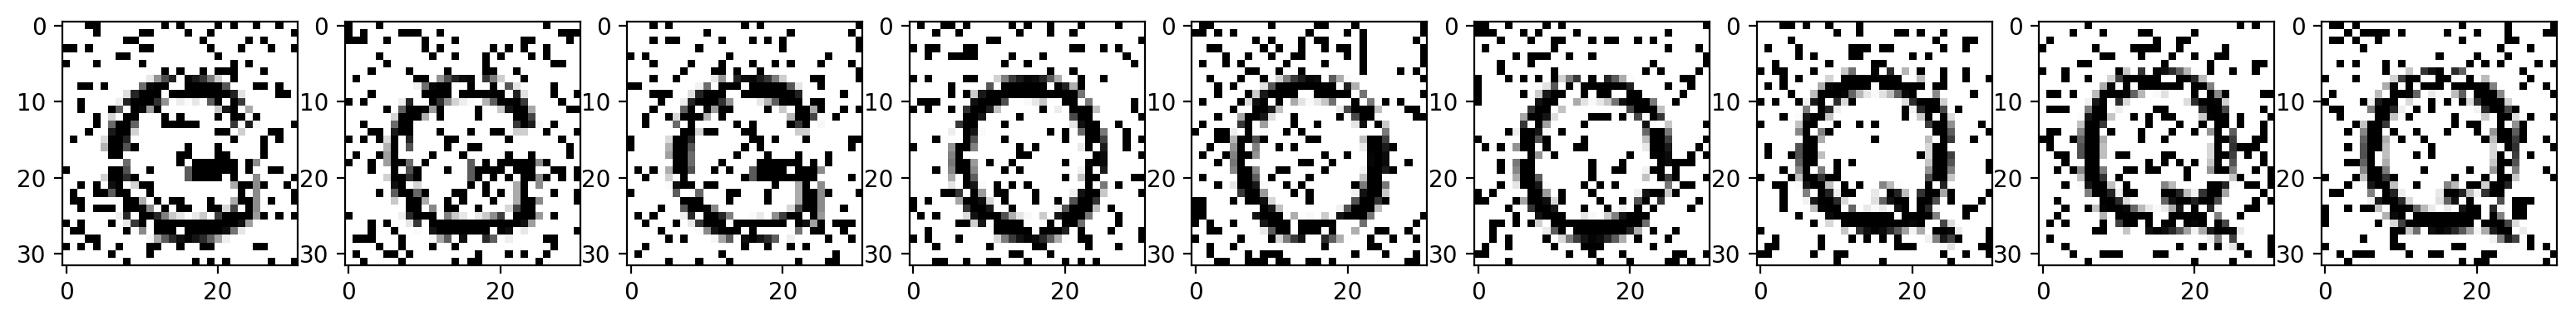
\includegraphics[width=\textwidth]{./images02/classification/GOQ-high-noise.png}}

  \subfloat[``G'', ``O'', and ``Q'' with 5\% noise.]{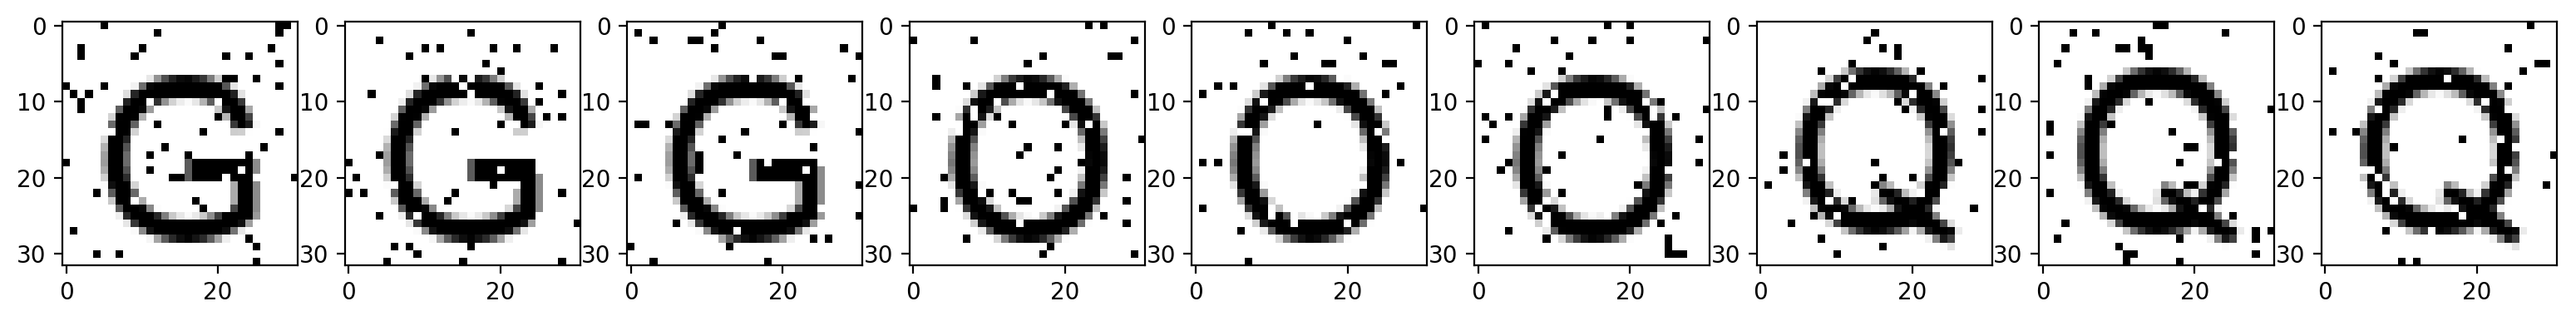
\includegraphics[width=\textwidth]{./images02/classification/GOQ-low-noise.png}}

  \caption{Images of different characters which may be confusing depending on the noise level.}
  \label{fig-classification-similarity}
\end{figure}

In the no noise scenario, the classifier has hit all characters, except letter ``l'' which was wrongly associated to the group of ``i''. We believe that it happened because the classifier had never seen an image with no noise and the difference between the images of ``l'' and ``i'' is smaller than the critical distance. So, both groups have been merged and it would converge to only one of them. In our simulation, it happened to be the group of ``i''.

In the low noise scenario, it has made few mistakes. It correctly classified all images but some from characters ``b'', ``e'', ``f'', ``l'', ``t'', and ``9''. It completely classified ``l'' images to the ``i'' group. In the other cases, it made just a few mistakes. See Figure \ref{fig-classification-low-noise-results} to check the images and their classification.

\begin{figure}[!htb]
  \centering
  \subfloat[Images from character ``b which were classified as {[b, b, b, h, b, o, b, h, b, b]}, respectively. It has made 3 misses.]{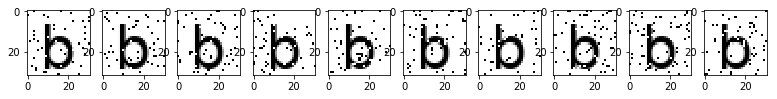
\includegraphics[width=\textwidth]{./images02/classification/low-noise-b.png}}

  \subfloat[Images from character ``e which were classified as {[e, e, e, e, e, e, e, e, o, e]}, respectively. It has made 1 miss. ]{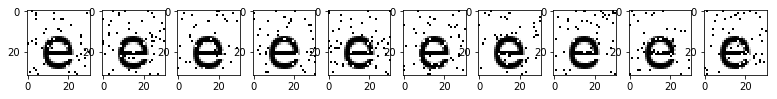
\includegraphics[width=\textwidth]{./images02/classification/low-noise-e.png}}

  \subfloat[Images from character ``f which were classified as {[i, f, f, I, I, I, f, f, f, f]}, respectively. It has made 4 misses. ]{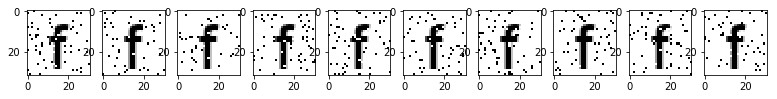
\includegraphics[width=\textwidth]{./images02/classification/low-noise-f.png}}

  \subfloat[Images from character ``l'' which were classified as {[i, i, i, i, i, i, i, i, i, i]}, respectively. It has missed them all, as if both groups have been merged. ]{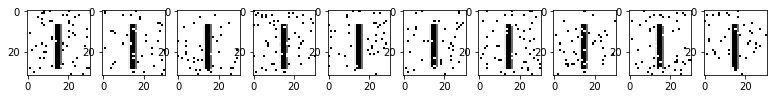
\includegraphics[width=\textwidth]{./images02/classification/low-noise-l.png}}

  \subfloat[Images from character ``t'' which were classified as {[t, t, t, t, t, t, t, i, t, t]}, respectively. It has made 1 miss. ]{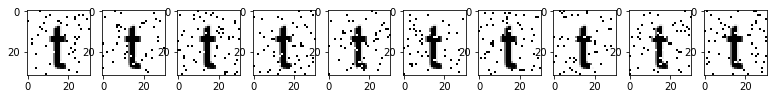
\includegraphics[width=\textwidth]{./images02/classification/low-noise-t.png}}

  \subfloat[Images from character ``9'' which were classified as {[9, 9, 0, 9, 9, 9, 0, 0, 9, 9]}, respectively. It has made 3 misses. ]{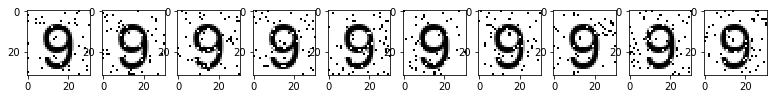
\includegraphics[width=\textwidth]{./images02/classification/low-noise-9.png}}

  \caption{Characters in the low noise scenario in which the classifier has made at least one mistake. In all the other cases, it correctly classified the images. We may notice that the groups of ``i'' and ``l'' have been completely merged by the classifier, because it cannot distinguish them, not even with no noise.}
  \label{fig-classification-low-noise-results}
\end{figure}

The high noise scenario is the most interesting, because, even in a high noise level, the classifier has hit most of the characters. It has hit all images for 44 out of 62 groups, and made at least one miss for the other 18 groups. The misses may be seen in details in Figure \ref{fig-classificiation-high-noise-misses}.

\begin{figure}[!htb]
  \centering
  \subfloat[Images from character ``B'' which were classified as {[S, B, B, B, B, B, B, B, B, B]}. It has made 1 mistake. ]{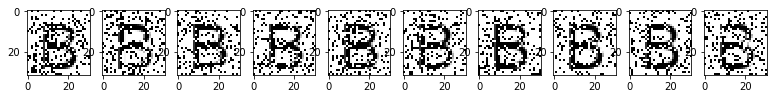
\includegraphics[width=\textwidth]{./images02/classification/high-noise-B.png}}

  \subfloat[Images from character ``O'' which were classified as {[G, G, O, O, O, O, O, O, O, O]}. It has made 2 mistakes. ]{\includegraphics[width=\textwidth]{./images02/classification/high-noise-O.png}}

  \subfloat[Images from character ``T'' which were classified as {[T, T, T, T, T, I, T, T, T, T]}. It has made 1 mistake. ]{\includegraphics[width=\textwidth]{./images02/classification/high-noise-T.png}}

  \subfloat[Images from character ``Y'' which were classified as {[Y, I, Y, Y, Y, Y, Y, Y, Y, Y]}. It has made 1 mistake. ]{\includegraphics[width=\textwidth]{./images02/classification/high-noise-Y.png}}

  \subfloat[Images from character ``b'' which were classified as {[o, o, o, b, o, h, h, b, b, o]}. It has made 7 mistakes. ]{\includegraphics[width=\textwidth]{./images02/classification/high-noise-b2.png}}

  \subfloat[Images from character ``c'' which were classified as {[c, c, c, c, c, o, c, c, c, o]}. It has made 2 mistakes. ]{\includegraphics[width=\textwidth]{./images02/classification/high-noise-c.png}}

  \subfloat[Images from character ``e'' which were classified as {[e, o, e, o, o, o, e, o, o, e]}. It has made 6 mistakes. ]{\includegraphics[width=\textwidth]{./images02/classification/high-noise-e.png}}

  \subfloat[Images from character ``f'' which were classified as {[I, I, I, I, i, I, I, I, I, I]}. It has missed them all. ]{\includegraphics[width=\textwidth]{./images02/classification/high-noise-f.png}}

\end{figure}
\begin{figure}[!htb]\ContinuedFloat

  \subfloat[Images from character ``i'' which were classified as {[i, i, i, I, i, i, i, i, I, i]}. It has made 2 mistakes. ]{\includegraphics[width=\textwidth]{./images02/classification/high-noise-i.png}}

  \subfloat[Images from character ``j'' which were classified as {[j, j, j, I, I, j, j, j, j, I]}. It has made 3 mistakes. ]{\includegraphics[width=\textwidth]{./images02/classification/high-noise-j.png}}

  \subfloat[Images from character ``l'' which were classified as {[I, i, I, I, I, I, i, I, I, i]}. It has missed them all. ]{\includegraphics[width=\textwidth]{./images02/classification/high-noise-l.png}}

  \subfloat[Images from character ``n'' which were classified as {[u, n, n, n, n, n, u, u, u, h]}. It has made 5 mistakes. ]{\includegraphics[width=\textwidth]{./images02/classification/high-noise-n.png}}

  \subfloat[Images from character ``q'' which were classified as {[q, q, q, q, q, q, q, q, q, g]}. It has made 1 mistake. ]{\includegraphics[width=\textwidth]{./images02/classification/high-noise-q.png}}

  \subfloat[Images from character ``t'' which were classified as {[I, r, I, i, I, i, i, i, I, i]}. It has missed them all. ]{\includegraphics[width=\textwidth]{./images02/classification/high-noise-t2.png}}

  \subfloat[Images from character ``1'' which were classified as {[1, I, 1, I, 1, 1, I, I, 1, I]}. It has made 5 mistakes. ]{\includegraphics[width=\textwidth]{./images02/classification/high-noise-1.png}}

  \subfloat[Images from character ``7'' which were classified as {[7, 7, 7, I, 7, I, I, 7, 7, 7]}. It has made 3 mistakes. ]{\includegraphics[width=\textwidth]{./images02/classification/high-noise-7.png}}

\end{figure}
\begin{figure}[!htb]\ContinuedFloat

  \subfloat[Images from character ``8'' which were classified as {[8, 6, 6, 6, 8, d, 8, 8, d, 6]}. It has made 6 mistakes. ]{\includegraphics[width=\textwidth]{./images02/classification/high-noise-8.png}}

  \subfloat[Images from character ``9'' which were classified as {[9, 0, 6, 0, 9, 0, 0, 9, 0, 0]}. It has made 7 mistakes. ]{\includegraphics[width=\textwidth]{./images02/classification/high-noise-9.png}}

  \caption{Characters in the high noise scenario in which the classifier has made at least one mistake. In all the other cases, it correctly classified the images.}
  \label{fig-classification-high-noise-misses}
\end{figure}

The critical distance plays an important role in the classification error. As we have 62 groups and each have been trained with 100 images, there were 6,200 writes to the memory. When an image is being classified, it will have to converge to a group, and the convergence depends on the distance between this image and the images from the training set, i.e, in the noise level.

These results show that the SDM may be used as a supervised classification algorithm. Although we do not believe that the mapping between images and bitstrings are even close to the way human cognition deals with images, we believe the results are interesting and useful to many possible real world problems.


\section{Results (iii): Supervised image noise filtering application}

Image noise filtering consists in removing the noise from an input, in out case an image. Our images are black \& white images and the noise is generated randomly flipping some of their pixels from black to while and vice versa. In Figure \ref{fig-filter-progressive-noise}, we may see an image with different levels of noise, from 0\% to 45\% in steps of 5\%. It makes no sense to apply 50\% of noise because it would absolutely randomize the image.

\begin{figure}[!htb]
\centering\includegraphics[width=\textwidth]{./images02/filter/progressive-noise.png}
\caption{Progressive noise into letter ``A'', from 0\% to 45\% in steps of 5\%.
\label{fig-filter-progressive-noise}}
\end{figure}

The images have 30 x 30 pixels, totaling 900 pixels per image. Each image is mapped into a 1,000 bit bitstring in which the bits are set according to the color of each pixel of the image. White pixels are equal to bit 0, and black pixels to bit 1. The 100 remaining bits are all set to zero. This is a bijective mapping (or one-to-one) from images and bitstrings, i.e., there is one, and only one, bitstring for each image, and vice versa.

In the learning phase, noisy images are generated and they are written into SDM chunked with their labels. The chunk was calculated using the exclusive or (XOR) operator. So, the image bitstring was written to the address of its bitstrings XOR its label bitstring --- \pyth{write(addr=bs_image ^ bs_label, datum=bs_image)}.

Finally, in order to remove the noise of a new image, first we have to classify it (possibly using the already presented classification algorithm), and then we just have to read from the chunked address until it converges.



\section{Results (v): The possibility of unsupervised reinforcement learning}

Reinforcement learning has increasing prominence in the media after AlphaZero has won all games from both the best chess grandmasters in the world and the best chess engines. What is incredible about these victories is that AlphaZero has almost no knowledge about chess game and has learned all its movement playing against itself for 4 hours. Basically, it knowns only the valid movements and had to learn everything from scratch, which it did using a reinforcement learning algorithm.

Reinforcement learning is a machine learning algorithm which learns from the rewards of its actions. So, it receives the game state as input, then it decides which action will be taken, and finally it learns from the rewards of all the actions it has chosen. In theory, it learns after each reward feedback it receives, improving its decision over time and presenting intelligent behavior. A positive reward would indicate that the chosen action should be encouraged. While a negative reward would indicate the opposite. In some algorithms, there may be a neutral reward which would indicate that the chosen action was neither positive nor negative. How each type of reward should be handled depends on each algorithm.

We have done some experiments with an SDM as a memory for a TicTacToe player. Basically, it receives the current board state and returns which action should be played. In the end of the game, it receives the sequences of boards and the winner, and is supposed to learn from them.

Our algorithm to decide what should be player is very simples: it read the current board from SDM. If the reading converges to another board, it chooses the movement which would bring the current board to the one read from SDM. If the reading does not converge, it just play randomly.

After a game has finished, it is time to learn from its decisions. Thus, if SDM wins the game, it will write the whole sequence of boards to SDM. Let $b_0, b_1, b_2, \dots, b_n$ be the board sequence of the game (see Figure \ref{fig-ttt-example}). Then it will write $b_0 \rightarrow b_1 \rightarrow b_2 \rightarrow \cdots \rightarrow b_n$, with possibly different weights for each transition. If it loses, it will reverse the board (replace X by O and vice versa), and will act as if it had won. Hence, it will learn which sequences lead to victory. When a new board appears, it may have already seen that situation and will decide according to the sequences which goes towards victory. This is our positive reward learning.

\begin{figure}
    \captionsetup[subfigure]{labelformat=empty}

    \subfloat[$b0$]{\begin{tabular}{p{\widthof{x}}|p{\widthof{x}}|p{\widthof{x}}}
     & & \\\hline  & & \\\hline  & &
    \end{tabular}}
    $\rightarrow$
    \subfloat[$b1$]{\begin{tabular}{p{\widthof{x}}|p{\widthof{x}}|p{\widthof{x}}}
     & & \\\hline  &x& \\\hline  & &
    \end{tabular}}
    $\rightarrow$
    \subfloat[$b2$]{\begin{tabular}{p{\widthof{x}}|p{\widthof{x}}|p{\widthof{x}}}
     & & \\\hline o&x& \\\hline  & &
    \end{tabular}}
    $\rightarrow$
    \subfloat[$b3$]{\begin{tabular}{p{\widthof{x}}|p{\widthof{x}}|p{\widthof{x}}}
    x& & \\\hline o&x& \\\hline  & &
    \end{tabular}}
    $\rightarrow$
    \subfloat[$b4$]{\begin{tabular}{p{\widthof{x}}|p{\widthof{x}}|p{\widthof{x}}}
    x& & \\\hline o&x& \\\hline  & &o
    \end{tabular}}
    $\rightarrow$
    \subfloat[$b5$]{\begin{tabular}{p{\widthof{x}}|p{\widthof{x}}|p{\widthof{x}}}
    x&x& \\\hline o&x& \\\hline  & &o
    \end{tabular}}
    $\rightarrow$
    \subfloat[$b6$]{\begin{tabular}{p{\widthof{x}}|p{\widthof{x}}|p{\widthof{x}}}
    x&x&o\\\hline o&x& \\\hline  & &o
    \end{tabular}}
    $\rightarrow$
    \subfloat[$b7$]{\begin{tabular}{p{\widthof{x}}|p{\widthof{x}}|p{\widthof{x}}}
    x&x&o\\\hline o&x& \\\hline  &x&o
    \end{tabular}}

    \caption{Example of a game with 7 movements in which X wins.\label{fig-ttt-example}}
\end{figure}

It is also important to learn when a draw happens --- after all, it is better to tie than to lose, right? In this case, the sequence of boards is also written to SDM, but with no weight at all. So, if the board has appeared both in a tie sequence and in a winning sequence, it would be more likely to choose the winning one because it was written with greater weight. This is our neutral reward learning.

Finally, we also want to prevent losing games. So, when it loses a game, it will stimulate movements different from the chosen ones. Thus, for each transition $b_k \rightarrow b_{k+1}$ made by its action, it will write all possible transitions from $b_k$ but $b_{k+1}$.

Internally, every board is mapped into a random bitstring and passed to SDM. Thus, SDM knows nothing about the boards themselves. It knowns only about their transition and which ones would lead to either a victory or a draw. As every two boards are orthogonal, SDM does not known whether two boards are consecutives or not. The only link between two boards is the transition written in SDM.

After all, SDM knowns nothing about the boards themselves and yet it may learn how to play TicTacToe.

In order to properly run the discussed algorithms, it is necessary to have two SDMs: a 0-fold and a 1-fold SDM. In the 0-fold SDM, every bitstring is written to its own address. In the 1-fold SDM, every bitstring points somewhere else. So, the transitions are written in the 1-fold SDM, while the boards themselves are written to the 0-fold SDM. The boards are written only once in the 0-fold, no matter how many times they appear. The transitions may be written more than once in the 1-fold SDM, because it would reinforce that transition.

In more details, the next movement decision consists in one read from the 1-fold SDM, resulting in a bitstring. Then this bitstring is used in an interative reading from the 0-fold SDM, which will converge to the bitstring associated with the next board. If it does not converge to any board, than SDM will choose a random movement and learn from it.

The weight used when writing a winning sequence is calculated using ...

--- talk about player generations ---

\subsection{Training}

It is an unsupervised algorithm because SDM learns playing against an opponent, who may be another SDM player, a human, or a player whose movements are always aleatory.

Thus, in order to train a SDM player, we just have to keep it playing over and over.


\begin{forest}
  TTT/.style args={#1:#2}{
    make tab/.expanded=\forestove{content},
    label={\pgfkeysvalueof{/forest/label position #1}:$#2$}
  },
  TTT*/.style={
    make tab=::/::/::,
    content/.expand once=%
    \expandafter\vphantom\expandafter{\romannumeral-`0\forestov{content}},
    draw=none,
    append after command={(\tikzlastnode.north) edge (\tikzlastnode.south)},
    for descendants={before computing xy={l*=1.2}},
  },
  th/.style=thick,
  for tree={node options=draw, inner sep=+0pt, parent anchor=south, child anchor=north}
%
[::/::/::, TTT=r:1
  [x::/::/::, TTT=r:-1
    [x::/::/::, TTT=r:-1
      [x::/::/::, TTT=r:-1
      ]
    ]
  ]
]
\end{forest}

\subsection{Results}



\chapter{Results (vi): Information-theoretical write operation}


\begin{figure}[h!]
  \centering
  \subfloat[$w_1(d), d \in \{ 1, 2, ..., n\}.$]{\includegraphics[width=3.2in]{./images02/new-images/Info-theory-a-global.jpeg}}

  \subfloat[$w_1(d)$ for the desired range. ]{\includegraphics[width=3.2in]{./images02/new-images/Info-theory-b-to-500.jpeg}}

  \subfloat[stepwise $\left \lfloor{w_1(d)}\right \rfloor$ for fast integer computation.]{\includegraphics[width=3.2in]{./images02/new-images/Info-theory-c-stepwise.jpeg}}

  \caption{Shannon write operation:  Computing the amount of information of a signal to each hard location in its access radius. (a) entirety of the space; (b) region of interest; (c) Fast integer computation is possible through a stepwise function.}
  \label{fig:info-theory-hypothesis}
\end{figure}



\begin{figure}[h!]
  \centering
  \subfloat[$w_2(d), d \in \{ 1, 2, ..., n\}.$]{\includegraphics[width=3.2in]{./images02/new-images/Info-theory-a-sum.jpeg}}

  \subfloat[$w_2(d)$ for the desired range. ]{\includegraphics[width=3.2in]{./images02/new-images/Info-theory-b-sum-range.jpeg}}

  \subfloat[stepwise $\left \lfloor{w_2(d)}\right \rfloor$ for fast integer computation.]{\includegraphics[width=3.2in]{./images02/new-images/Info-theory-c-sum-stepwise.jpeg}}

  \caption{SOON TO BE DEPRECATED.  Shannon write operation:  Computing the sum of low-likelihood signals. (a) entirety of the space; (b) region of interest; (c) Fast integer computation through a stepwise function. }
  \label{fig:info-theory-sum-hypothesis}
\end{figure}




\begin{figure}[h!]
  \centering
  \subfloat[Kanerva's model]{\includegraphics[width=\linewidth]{./images02/new-images/kanerva-15iter-reads.jpeg}}

  \subfloat[Write process weighted by the amount of information contained in the distance between the written bitstring and each hard location]{\includegraphics[width=\linewidth]{./images02/new-images/info-theory-15iter-reads.jpeg}}


  \caption{(a) and (b) show the behavior of the critical distance under Kanerva's model and the information-theoretic one, respectively.}
  \label{fig:info-theory-experiments}
\end{figure}



\begin{figure}[h!]
  \centering
  \subfloat[$w_2(d), d \in \{ 1, 2, ..., n\}.$]{\includegraphics[width=3.2in]{./images02/new-images/Info-theory-shannon.jpeg}}

  \subfloat[$w_2(d)$ for the desired range. ]{\includegraphics[width=3.2in]{./images02/new-images/Info-theory-shannon-region.jpeg}}

  \subfloat[stepwise $\left \lfloor{w_1(d)}\right \rfloor$ for fast integer computation.]{\includegraphics[width=3.2in]{./images02/new-images/Info-theory-shannon-stepwise.jpeg}}

  \caption{Shannon write operation:  Computing the amount of information of a signal to each hard location in its access radius. (a) entirety of the space; (b) region of interest; (c) Fast integer computation is possible through a stepwise function.}
  \label{fig:info-theory-hypothesis}
\end{figure}



My advisor, Alexandre Linhares, has proposed another read operation: an information-theoretical weighted reading. In it, the sum of the counter's value is weighted based on the distance between each hard-location's address and the reading address. The logic behind it is to vary the importance of each hard-location inside the circle.  It is only natural that one encodes an item in closer hard locations with a stronger signal, and a natural candidate for this signal function is the amount of information contained in the distance between the item and each hard location.  Closer hard locations have lower probabilies and therefore should encode more information.

Consider the following. Information Theory \citep{cover2012elements} let us compute the precise amount of information in an event, when given its probability $p$, through the measure of \emph{self-information}:\\

$I(p)= -log_2(p).$ \\

Now, given any two $n$-sized bitstrings, the probability of their Hamming distance being $d$ is given by,


$p(H=d)= {2^{-n} \binom{n}{d} }$ \\

And the probability of it being at most $d$ is \\

$p(H\leq d)= 2^{-n} {\displaystyle\sum_{i=0}^{d}{\binom{n}{i}}}  $, \\

and, consequently,

$p(H\geq n-d)=2^{-n}{\displaystyle\sum_{i=n-d}^{n}{\binom{n}{i}}  }$, \\

$p(d+1 \leq H \leq n-d-1)=2^n - 2^{1-n}{\displaystyle\sum_{i=0}^{d}{\binom{n}{i}}, \forall d<n/2}$. \\

Hence the weighted write would, on each hard location, sum (or subtract) the following:  \\

$w(d) = -\log_2 \left( 2^{-n} \binom{n}{d} \right) = n - \log_2 \binom{n}{d}$, as seen in Figure \ref{fig:info-theory-hypothesis}.

It is easy to interpret this data though a binary tree approach.  How many binary questions would be needed to precisely define a bitstring?

Another possibility would be to use the sum of all distances closer (and less likely) locations within the weighting function $w(d)$,

$w(d) = -\log_2 \left( 2^{-n} \displaystyle\sum_{i=0}^{d}{\binom{n}{i}} \right) = n - \log_2 \displaystyle\sum_{i=0}^{d}{\binom{n}{i}}$. \\

This can be seen in \ref{fig:info-theory-sum-hypothesis}.

The initial results of this \emph{Shannon write} operation can be seen in Figure \ref{fig:info-theory-experiments} and seem promising. It seems that the critical distance increases by a number of bits.  Note that 10 additional bits imply an attractor $2^{10}$ of the size of the original. Another point to keep in mind is that, since the modulus of the vectors are not uniform in this approach, that the shape of the attractor may have asymmetries.

But, qualitatively, they seem disappointing.  HEATMAPFIGs


Note, finally, that this is not the first time in which a weighted function has been applied to writing in SDM --- \citet{hely1997new} suggest a rather complex spreading model based on floating point signals in the interval [0.05, 1.0] --- they were, however, only able to test their model with 1,000 hard locations.








\chapter{Conclusion}

Sparse Distributed Memory is a viable model of human memory, yet it does require researchers to (re-)implement a number of parallel algorithms in different architectures.

We propose to provide a new, open-source, cross-platform, highly parallel framework in which researchers may be able to create hypotheses and test them computationally through minimal effort. The framework is well-documented for public release at this time (http://sdm-framework.readthedocs.io), it has already served as the backbone of Chada's Ph.D. thesis. The single-line command ``pip install sdm'' will install the framework on posix-like systems, and single-line commands will let users test the framework, generate some of the figures from Kanerva's theoretical predictions in their own machines, and --- if interested enough ---, test their own theories and improve the framework, and the benchmarks used to evaluate the framework, in open-source fashion. It is our belief that such work is a necessary component towards accelerating research in this promising field.

\section{Future work}

Here are interesting questions that have been considered during this work, but have had to be left for future research.

\subsection{Multiple levels}


\subsection{i versus l}


\subsection{Magic numbers}

Kanerva suggests, in his book, the use of 1,000 dimensions and 1,000,000 hard locations.  More recently, he suggested the use of 10,000 dimensions, and on personal discussions suggested that this should be a minimum; as he has been concerned in latent semantic analysis and seems to be the proper scale in that application.

Each parameter set choice like this will lead to particular numbers --- many of them emergent---, such as the access radius size, critical distance, and so forth.

One intriguing question here is:  is there a `better' number of dimensions and of hard locations?  If so, can such numbers better studied analitically, or numerically?

How should these parameters be compared?  What are the tradeoffs that should be considered?  What are the `best' benchmarks possible?

\subsection{Classification with context using sequences --- for words instead of only letters}










\subsection{Symmetrical, rapidly accessible, Hard Locations}

A hypercube with n dimensions can be divided by two hypercubes with $n-1$ dimensions. Is there an algorithm that separates the area of each hard-location in such a form that there exists a function mapping each bitstring in $\{0,1\}^n$ to the set of hard locations it `belongs to'?  Though this would break Kanerva's assumption of a randomly yet uniformly distributed set of hard locations --- for a perfectly symmetrical set of hard locations ---, there could be large performance gains if such a mapping function from a bitstring to its corresponding set of nearest hard locations exists.

$\forall b \in \{ 0,1\} ^n$, we want an algorithm $A$ that yields the particular list of hard locations for $b$ and all hard locations respect the desired properties of the memory.  A reduction from measuring the distance to $10^6$ hard locations to a computation of $~ 10^3$ hard locations might yield astonishing performance gains, depending, of course, on our optimistic assumptions concerning existence and complexity of such algorithm.

At large scales of computing, the very ability to perform some experiments is a function of sheer performance. The horizon of experiments --- and possibly of knowledge --- expands \emph{as a function of computational demands}. More on this in my closing words.

\section{Seeing farther}

Let us revisit, in these concluding thoughts, the emphasis employed over speed of computation.  At first sight, that might seem like a typical objective of efficiency in computer science. But we are not only interested in the computer science effects here --- the ambition is different. More important than this `computer-sciency' goal, i.e., a beautiful, clean, efficient algorithm with the primary effect of enhanced speed, however, is the secondary effect on the sociology of science:  \emph{We can see farther}.

If

We have generated a Docker image, which makes it even easier to explore the framework. After running the container, a Jupyter Notebook is available with sdm-framework and other tools already installed.


All the simulations and graphics generated in this thesis are promptly available to be re-executed and explored by those interested. We invite readers to take a look and explore a little bit.

\subsection{From theory to a platform.}


Platforms in the history of computing.


Opens 10 doors.


% TODO Include in the to do list simulations based on the suggestion of Murilinho.

\chapter{Appendix}
%\section{Generating Kanerva's table 7.3}

%\includepdf[
%  pages=-,
%  pagecommand={\pagestyle{headings}},
%  %addtotoc={1,section,1,Quilling Shapes,sec:shapes}
%]{./Chapter02-SDM/Kanerva-Table-7.3/Kanerva-Table-7_3.pdf}
